%%
%% Author: Alexander
%% 18.02.2018
%%

% Preamble
\documentclass[a4paper,12pt]{article}

% Packages
\usepackage[14pt]{extsizes}
\usepackage{mathtext}
\usepackage[T2A]{fontenc}
\usepackage[utf8]{inputenc}
\usepackage[pdftex]{hyperref}
\usepackage[russian]{babel}
\usepackage{amsmath}
\usepackage{longtable}
\usepackage{amsfonts}
\usepackage{amssymb}
\usepackage{graphicx}
\usepackage[left=2cm,right=2cm,
    top=2cm,bottom=2cm,bindingoffset=0cm]{geometry}
\usepackage{color}
\usepackage{gensymb}
\linespread{1.25}

\usepackage{enumitem}
\setlist[enumerate]{label*=\arabic*.}

\usepackage{indentfirst}

\usepackage{titlesec}

% Document
\begin{document}

    \begin{titlepage}

        \begin{center}
            \begin{Large}
            МГТУ\ им.\ Н.Э.\ Баумана\\
            \end{Large}
            \begin{large}
            \vspace{6cm}
            Черновик диплома\\
            \vfill
            \end{large}
        \end{center}

        \begin{flushright}
            \begin{large}
            Жигалкин А.С.\\
            Группа: Э3-122\\
            \vspace{2cm}
            \end{large}
        \end{flushright}

        \begin{large}
            \begin{center}
           Москва\ 2018
            \end{center}
        \end{large}

    \end{titlepage}


    \tableofcontents
    \newpage

%	
%   
%   
%   
%   
%   

    \section{ВВЕДЕНИЕ}
    Газотурбинные имееют достаточно широкое примение в энергетике в качестве привода электрогенератора.
    Основными особенностями ГТУ по сравнению с энергетическими установками других типов являются:
    \begin{enumerate}
        \item Высокая маневренность.
        \item Компактность.
        \item Малый срок ввода в эксплуатацию.
        \item Низкая потребность в воде.
        \item Относительно низкий капитальные затраты.
        \item Относительно низкая экономичность.
        \item Относительно невысокая потребность в смазочных материалах (по сравнению с двигателями
        внутреннего сгорания)
    \end{enumerate}
    Данные особенности определяют основные области применения ГТУ.
    Они используются как правило для покрытия пиковых нагрузок в составе электростанций или для
    энергоснабжения промышленных предприятий, морских платформ, небольших населенных пунктов и т.п.
    Энергетических установок, которые обладали бы в перечисленных областях существенными преимуществами перед ГТУ, на
    данный момент не существует.
    Поэтому создание новых газотурбинных установок, обладающих большей экономичностью,
    меньшими капитальными затратами, большей материалоемкостью, чем существующие, является актуальной задачей.
    В данной выпускной квалификационной работе эта задача будет решаться для класса мощности 16 МВт.

    Проектируемая ГТУ будет обладать большей, чем у конкурентов, начальной температурой газа в цикле
    ($ 1523\ К $).
    Это потребует проектирования более совершенной системы охлаждения, но позволит добится большей экономичности и
    меньшей металлоёмкостью, за счет возможности уменьшить диаметральный размер лопаточных машин.
    Установка будет выполнена по двухвальной схеме со свободной турбиной.
    Энергоблок на основе ГТУ будет выполнен по модульному принципу, что обеспечит удобство транспортировки установки с
    завода-изготовителя и высокую скорость строительства блока.

    \newpage

    \section{Техническое задание на диплом.}
    Спроектировать газотурбинную установку мощностью 16 МВт, предназначенную для
    привода электрогенератора.
    Топливо - природный газ.

    \newpage

    \section{Обоснование выбора схемы и параметров ГТУ.}

    \subsection{Обзор существующих энергетических приводных ГТУ в классе мощности 16 МВт.}

     Ниже будут рассмотрены следующие ГТУ энергетического назначения в классе мощность 16 МВт:
    \begin{enumerate}
        \item Установка ГТЭ-16ПА фирмы АО «ОДК-Пермские моторы».
        \item Установка SGT-500 фирмы Siemens.
        \item УстановкаTitan 130 фирмы Solar Turbines Inc.
        \item Установка АЛ-31СТЭ фирмы ПАО «ОДК-УМПО».
        \item Установка Т16 фирмы АО «РЭП Холдинг».
    \end{enumerate}

    \paragraph{Установка ГТЭ-16ПА.}

    \begin{figure}[h!]
        \centering
        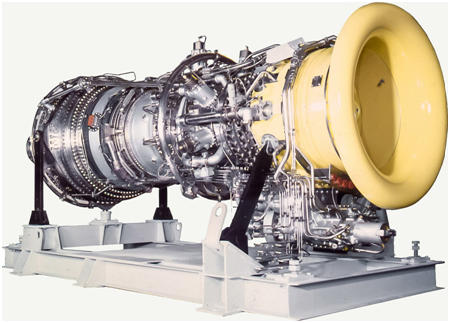
\includegraphics[scale=1]{./pictures/GTE-16PA.png}
        \caption{Фотография установки ГТЭ-16ПА.}
        \label{pic_gte_16pa}
    \end{figure}

    Газотурбинная установка ГТЭ-16ПА (рис.~\ref{pic_gte_16pa}) создана на базе двигателя ПС-90ЭУ-16А.
    Этот новый двигатель разработан в рамках сотрудничества ОАО «Авиадвигатель» с фирмой Pratt\&Whitney (США).
    Установка выполнена по двухвальной схеме с силовой турбиной.
    Она состоит из 14-ти ступенчатого осевого компрессора, камеры сгорания, 2-х ступенчатой турбины
    компрессора и 4-х ступенчатой силовой турбины.
    Эффективный КПД установки составляет 36,6\%~\cite{aviadvig}.
    С целью повышения эксплуатационной технологичности и экологической безопасности на двигатель
    устанавливается система электрозапуска.
    Главным конструктивным отличием ПС-90ЭУ-16А от других промышленных двигателей, разработанных
    ОАО «Авиадвигатель» за последние 12-13 лет, является четырехступенчатая свободная силовая турбина с номинальной
    частотой вращения 3000 об/мин~\cite{gtes-16pa}.
    Выходной вал является приводом синхронного турбогенератора Т-16-2РУХЛ3 производства ОАО «Привод» (г. Лысьва).
    Уменьшение частоты оборотов дает возможность отказаться от использования редуктора, снизив тем самым
    эксплуатационные затраты и повысив надежность всей газотурбинной установки в целом.
    Вместо оптимальной по аэродинамике пятиступенчатой силовой турбины было принято решение о
    проектировании четырехступенчатой.
    Увеличение аэродинамической нагрузки на ступень и снижение примерно на 1\% КПД силовой турбины от максимально
    достижимой величины позволило заведомо снизить суммарные затраты потенциальных заказчиков почти на 20\%~\cite{raz_konstr_perm}
    Для снижения материалоемкости и веса ГТЭ-16ПА был использован богатый опыт разработки авиационных турбин.
    В результате масса ротора двигателя ПС-90ЭУ-16А, несмотря на увеличение диаметра и количества ступеней,
    оказалась равной массе ротора ПС-90ГП-2, что позволило обеспечить высокую степень унификации трансмиссий.~\cite{raz_konstr_perm}


    \paragraph{Установка SGT-500.}

    \begin{figure}[h!]
        \centering
        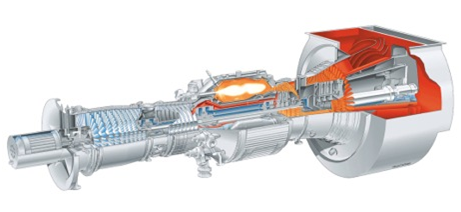
\includegraphics[scale=1.0]{./pictures/SGT-500.png}
        \caption{Схема установки SGT-500.}
        \label{pic_stg_500}
    \end{figure}

    SGT-500 (GT35C) (рис.~\ref{pic_stg_500}) мощностью 17 МВт применяется на различных объектах, где наиболее важными параметрами
    являются: базовая нагрузка, способность работать на различных видах  топлива, простота технического
    обслуживания.
    Наряду с производством  электроэнергии, SGT-500 широко используется как механический
    привод  мощностью 23290 л.с. Может работать на различных видах тяжелого топлива.
    Относительно невысокая температура газов перед турбиной способствует снижению деградации характеристик и
    увеличению межремонтного ресурса ГТУ (80 000 ч), а модульный принцип конструкции позволяет
    быстро производить замену узлов.
    Модульная и компактная конструкция турбины SGT-500 облегчает обслуживание на месте — можно быстро менять целые модули.
    В турбине SGT-500 установлен двухвальный газогенератор: на валу низкого давления установлен
    10-ступенчатый компрессор низкого давления и 2-ступенчатая турбина низкого давления.
    На валу высокого давления установлен 8-ступенчатый компрессор высокого давления и
    1-ступенчатая турбина высокого давления.
    Обороты трехступенчатой турбины равны 3600 мин-1 при генерации электроэнергии и 3450 мин-1 при
    приводе механических устройств.
    Для повышения эффективности между статором и ротором
    силовой турбины устанавливается регулятор зазора между корпусом и концами лопаток.
    Турбина поставляется с обычной системой сжигания топлива либо с системой сухого снижения
    токсичности выхлопных газов (DLE).
    Обе системы поддерживают работу на двух видах топлива, а система DLE обеспечивает крайне низкий
    уровень выбросов $NO_{x\leq}$42 ppmV.Все подшипники газодинамические,
    с шарнирно-закрепленным сегментом подпятника.
    Пусковой электродвигатель соединен с ротором компрессора низкого давления.~\cite{sgt-500}

    \paragraph{Установка Titan 130.}

    \begin{figure}[h!]
        \centering
        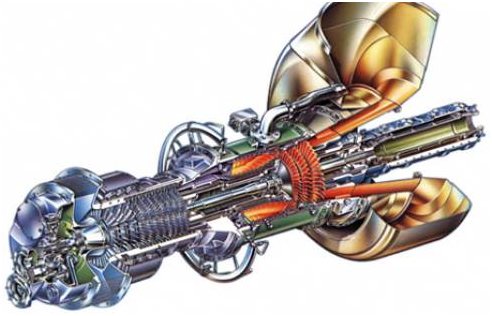
\includegraphics[scale=1.0]{./pictures/Titan_130.png}
        \caption{Схема установки Titan 130.}
        \label{pic_titan130}
    \end{figure}

    Titan 130 (рис.~\ref{pic_titan130}) – установка мощностью 16,5 МВт.
    Выполнена по одновальной схеме.
    Состоит из 14-ти ступенчатого компрессора со степенью сжатия 17,1, кольцевой камеры сгорания с
    системой сухого снижения токсичности выхлопных газов и 3-х ступенчатой силовой турбины.
    Частота вращения вала силовой турбины 11220 об/мин.
    Электрический КПД установки составляет 35,5 \%.~\cite{titan130}

    \paragraph{Установка АЛ-31СТЭ.}

    \begin{figure}[h!]
        \centering
        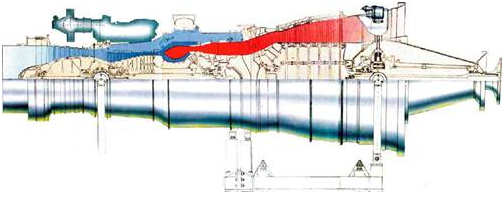
\includegraphics[scale=1.0]{./pictures/AL-31ST.png}
        \caption{Схема установки АЛ-31СТЭ.}
        \label{pic_al_31st}
    \end{figure}

    Также в классе мощности 16 МВт можно выделить двигатель АЛ-31СТЭ,
    конвертированный из двухконтурного двигателя самолета СУ-27 АЛ-31Ф.
    Схема данного двигателя представлена на рис.~\ref{pic_al_31st}.
    Данный двигатель также состоит из газогенератора и модуля свободной турбины, что облегчает ее модульный монтаж.
    Мощность на валу силовой турбины составляет 18 МВт, КПД – 38,1\%.
    Двигателю АЛ31-СТЭ свойственен невысокий по меркам стационарной техники ресурс в 75 000 ч, что
    связано с назначением двигателя – прототипа.
    Двигатель прототип АЛ-31Ф был разработан для высокоманевренного самолета СУ-27, и при его проектирование
    в основном велось на условие максимизации тяги.
    Низкоэмиссионная камера сгорания установки обеспечивает уровень вредных выбросов оксида азота
    менее 40 ppm и оксида углерода менее 80 ppm.
    Высокое совершенство рабочего процесса в камере сгорания достигнуто за счет предварительного
    смешения топливного газа в модуле-гомогенизаторе и поддержания оптимальных значений коэффициентов
    избытка воздуха в первой и второй зонах горения. Окружная неравномерность поля температуры на выходе из
    камеры сгорания снижена в 2 раза по сравнению с исходной камерой сгорания.~\cite{al-31st}
    Модульная конструкция привода обеспечивает замену узлов без
    дополнительных работ по подгонке, балансировке и испытаниям.~\cite{al-31st}


    \paragraph{Установка Т16.}
    \begin{figure}[h!]
        \centering
        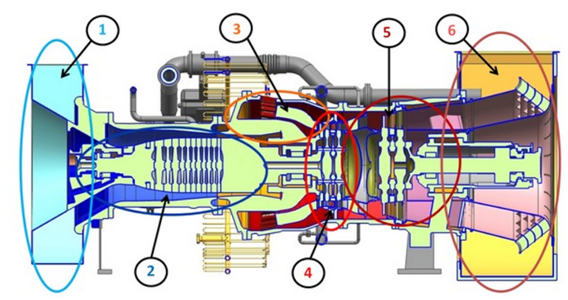
\includegraphics[scale=1.0]{./pictures/T16.png}
        \caption{Продольный разрез турбины Т16.}
        \label{pic_t16}
    \end{figure}

    Также в рассматриваемом классе мощностей присутствует одна из новейших российских газотурбинных электростанций:
    ГТЭ-16 на базе стационарной газотурбинной установки Т16 производства компании «РЭП Холдинг» в сотрудничестве с
    GEOil\&Gas.

    Схема установки представлена на рис.~\ref{pic_t16}.
    Данная установка конструктивно выполнена по двухвальной схеме со свободной турбиной.
    Отличительной особенностью установки является высокий ресурс (200 000 ч) ~\cite{rep_holding} при высоком значении КПД (37 \%)
    и низком уровне эмиссии оксидов азота (менее 25 ppm)~\cite{turbineT16}.
    Камера сгорания выполнена по противоточной схеме.
    Для поддержания высокого КПД на режимах частичной мощности (от 20\% до 100\% номинальной мощности)
    применяются поворотные направляющие аппараты трех ступеней компрессора, а также поворотный сопловой
    аппарат первой ступени силовой турбины~\cite{turbineT16}.
    Модули высокого и низкого давления располагаются на отдельных рамах и монтируются в корпусе на
    подвижных опорах, что позволяет извлекать их из общего корпуса установки в боковом направлении
    (рис.~\ref{pic_t16_tb_roll_out}-~\ref{pic_t16_pt_roll_out}) по отдельности или совместно.
    Такое конструктивное решение значительно упрощает обслуживание установки~\cite{turbineT16}.

    \begin{figure}[h!]
        \centering
        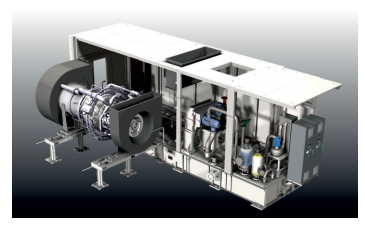
\includegraphics[scale=1.0]{./pictures/T16_tb_roll-out.png}
        \caption{Выкатка турбоблока целиком.}
        \label{pic_t16_tb_roll_out}
        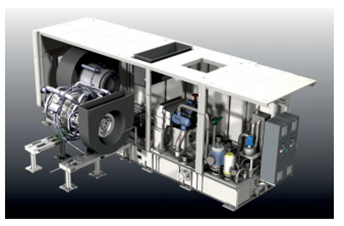
\includegraphics[scale=1.0]{./pictures/T16_gg_roll-out.png}
        \caption{Выкатка газогенератора.}
        \label{pic_t16_gg_roll_out}
        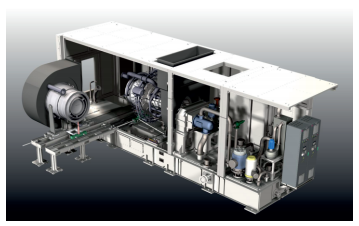
\includegraphics[scale=1.0]{./pictures/T16_pt_rool-out.png}
        \caption{Выкатка модуля силовой турбины.}
        \label{pic_t16_pt_roll_out}
    \end{figure}


    \subsection{Выбор схемы и параметров проектируемой ГТУ.}

    \begin{longtable}{|p{3.5cm}|p{2.2cm}|p{2.2cm}|p{2.2cm}|p{2.2cm}|p{2.2cm}|}

            \caption{Параметры различных установок в классе мощности 16 МВт.}\\

            \hline \label{engines16MW}
            Установка & ГТЭ-16ПА & SGT-500 & Titan 130 & АЛ-31СТЭ & T16 \\
            \hline
            Производитель & АО «ОДК-Пермские моторы» & Siemens & Solar Turbines Inc. & ПАО «ОДК-УМПО» & АО «РЭП Холдинг» \\
            \hline
            Мощность на валу силовой турбины, МВт &	16,8 & 19,7 & 16,96 &18 & 16,5 \\
            \hline
            Эффективный КПД, \% &	36,6 &	34,7 &	36,6 &	38,1 &	37,0 \\
            \hline
            Мощность на валу клеммах генератора, МВт & 16,3 &	19,1 &	16,45 &	17,46 &	16 \\
            \hline
            Электрический КПД, \% &	35,5 &	33,7 &	35,5 &	37 &	35,86 \\
            \hline
            Схема &	2Н &	3Н &	1Б &	3Н &	2Н \\
            \hline
            Степень повышения давления в компрессоре &	19,9 & 13 & 17,1 & \_ &	19,0 \\
            \hline
            Температура выхлопных газов, $^\circ C$ &	481 &	369 &	490 &	515 &	490 \\
            \hline
            Расход выхлопных газов, кг/с &	56,3 &	97,9 &	54,7 &	67 &	54,3 \\
            \hline
            Частота вращения силовой турбины, об/мин &	3000 &	3600 &	11220 &	3000 &	7800 \\
            \hline
            Температура газа перед турбиной, $^\circ C$ &	1410 &	1150 &	1400 &	\_ &	1410 \\
            \hline
            Число ступеней компрессора &	14 &	10+8 &	14 &	4+10 &	12 \\
            \hline
            Число ступеней турбины &	2+3 &	1+2+3 &	3 &	1+1+5 &	2+2 \\
            \hline
            Ресурс до капитального ремонта, ч & 20000 & 80000 & \_ & 25000 & \_ \\
            \hline
            Назначенный ресурс, ч & 100000 & 160000 & \_ & 75000 & 200000 \\
            \hline
        \end{longtable}

    Как видно из таблицы ~\ref{engines16MW} максимальный уровень температур газа для установок рассматриваемого
    класса мощности находится в районе 1400 К.
    Большинство установок, как конвертированные из авиационных, так и вновь создаваемые установки энергетического
    назначения (T16), выполнено по двухвальной схеме со свободной турбиной.
    Для перспективной установки целесообразно выбрать такую же схему, но большую начальную температуру газа,
    так как ее увеличение при заданной мощности позволяет добиться меньшего расхода рабочего тела, а, следовательно,
    и меньших диаметральных размеров, что, в свою очередь, означает уменьшнение массы.
    Также увеличение температуры газа после камеры сгорания ведет к росту эффективного КПД установки.
    Для проектируемой установки было выбрано значение начальной температуры газа $T_г^* = 1523\ К$.
    Это выше, чем у конкурентов.
    Поэтому вышеуказанные преимущества будут обеспечены.
    Но при этом возникнет необходимость проектирования более эфективной системы охлаждения, а
    возможно и применения более эффективных защитных покрытий и жаростойких материалов для лопаточных
    аппаратов турбины.
    Это несколько увеличивает стоимоть ГТУ, но как показывает опыт, несмотря на это, удельная стоимость установки
    при увеличении температуры газа при принятых методах охлаждения существенно снижается ~\cite{manushin_eliseev_proektirovanie}.

    \newpage

    \section{Расчетно-конструкторская часть}

    \subsection{Расчет цикла установки.}

    \subsubsection{Параметры электрогенератора.}

%    
\begin{enumerate}
	\item Электрогенератор: Т-16-2Р УХЛ3.1.
	\item Мощность электрогенератора: $N_{эг} = 16.0\ МВт$.
	\item КПД электрогенератора: $\eta_{эг} = 0.978$
	\item Мощность на валу электрогенератора: $N = \frac{N_{эг}}{\eta_{эг}} = 16.36\ МВт$.
\end{enumerate}


    \subsubsection{Исходные данные для расчета цикла.}
%    
\begin{enumerate}

	\item Давление окружающей среды: $p_{н} = 0.1013 \cdot 10^6\ Па$.
	\item Температура окружающей среды: $T_{н} = 288\ К$.
	\item Мощность на валу нагрузки: $ N = 16.36 \cdot 10^6\ МВт $.
	\item Температура торможения после камеры сгорания: $T_г^* = 1523\ К$.
	\item Политропический КПД компрессора: $\eta^*_{к п} = 0.89 $.
	\item Политропический КПД турбины компрессора: $\eta^*_{ткп} = 0.884$.
	\item Политропический КПД силовой турбины: $\eta^*_{тсп} = 0.884$.
	\item Низшая теплота сгорания топлива (природный газ): $Q^р_н = 48.412 \cdot 10^6\ Дж/кг$.
	\item Теоретически необходимая масса воздуха: $l_0 = 16.683\ кг/кг$.

	\item Степень сохранения полного давления во входном патрубке: $\sigma_{вх} = 0.99$.
	\item Степень сохранения полного давления в выходном патрубке: $\sigma_{вых} = 0.99$.
	\item Степень сохранения полного давления в камере сгорания: $\sigma_г = 0.98$.
	\item Коэффициент полноты сгорания: $\eta_г = 0.995 $.
	\item Относительный расход на охлаждение лопаток: $g_{охл} = 0.12$.
	\item Относительный расход на прочие нужды: $g_{ут} = 0.03$.
	\item Относительный расход воздуха, возвращаемого перед силовой турбиной: $g_{воз} = 0.12$.
	\item Температура возвращаемого перед силовой турбиной воздуха: $T_{воз} = 800\ К$.
	\item Механический КПД на валу турбины компрессора: $\eta_{м.тк} = 0.99$.
	\item Механический КПД на валу силовой турбины: $\eta_{м.тс} = 0.99$.
	\item КПД редуктора: $ \eta_р = 0.99$.
	\item Скорость на выходе из выходного устройства: $ c_{вых} = 100 $

\end{enumerate}


    \subsubsection{Вариантные расчеты и выбор параметров.}
    Для выбора степени повышения давления и обоснования выбора начальной температуры газа была проведена серия расчетов
    для различных значений $\pi_к^*$ в цикле при трех различных значениях $T_г^*$: выбранном, на 50 К больше и на 50 К
    меньше выбранного.
    В результате были получены зависимости удельного расхода топлива $C_e$, эффективного КПД $\eta_e$ и расхода
    воздуха на входе в компрессор $G_в$ и мощности, отнесенной к расходу в компрессоре, $\bar{N}_e$
    от степени повышения давления в компрессоре.
    Данные зависимости предствлены на рис.~\ref{cycle_eta},~\ref{cycle_C_e},~\ref{cycle_N_e_sp},~\ref{cycle_G_air}.
    Также была произведена оценка наименьших размеров лопаточных аппаратов.
    Для турбины - это размер лопатки СА первой ступени турбины компрессора, для компрессора - размер лопатки
    последней ступени.
    Размер СА и средний диаметр турбины компрессора на входе представлены на рис.~\ref{cycle_l_sa1} и~\ref{cycle_D_av1}.

    \begin{figure}[h!]
        \centering
        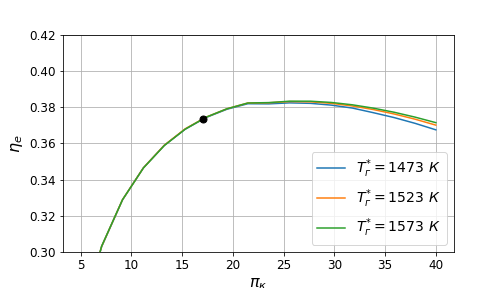
\includegraphics[scale=0.8]{../plots/cycle_eta_e.png}
        \caption{Зависимость КПД цикла от степени повышения давления.}
        \label{cycle_eta}

        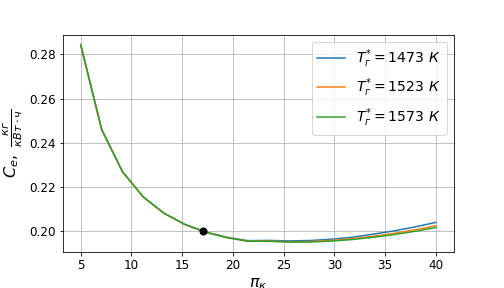
\includegraphics[scale=0.8]{../plots/cycle_C_e.png}
        \caption{Зависимость удельного расхода топлива в цикла от степени повышения давления.}
        \label{cycle_C_e}
    \end{figure}

    \begin{figure}[h!]
        \centering
        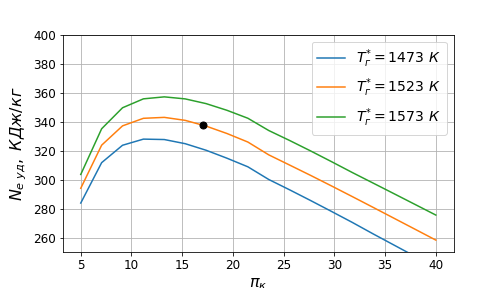
\includegraphics[scale=0.8]{../plots/cycle_N_e_sp.png}
        \caption{Зависимость удельной мощности от степени повышения давления.}
        \label{cycle_N_e_sp}

        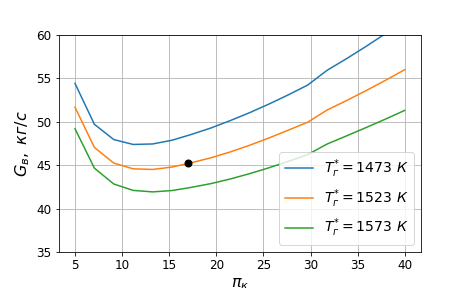
\includegraphics[scale=0.8]{../plots/cycle_G_air.png}
        \caption{Зависимость расхода воздуха на входе от степени повышения давления.}
        \label{cycle_G_air}
    \end{figure}

    \begin{figure}[h!]
        \centering
        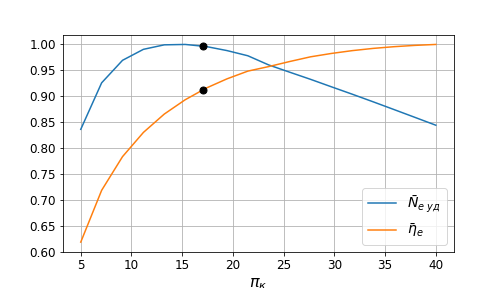
\includegraphics[scale=0.8]{../plots/cycle_N_e_sp_rel_eta_e_rel.png}
        \caption{Зависимости КПД и удельной мощности в относительных координатах от степени повышения давления.}
        \label{cycle_N_e_sp_rel_eta_e_rel}

        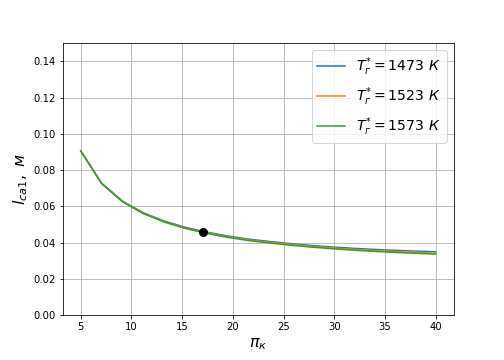
\includegraphics[scale=0.8]{../plots/cycle_l_sa1.png}
        \caption{Зависимость длина лопатки СА первой ступени турбины компрессора от степени повышения давления.}
        \label{cycle_l_sa1}
    \end{figure}

    \begin{figure}[h!]
        \centering
        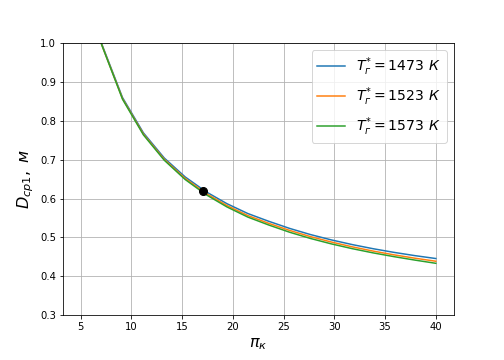
\includegraphics[scale=0.8]{../plots/cycle_D_av1.png}
        \caption{Зависимость среднего диаметра на входе в турбину компрессора от степени повышения давления.}
        \label{cycle_D_av1}
    \end{figure}

    С точки зрения максимального уменьшения диаметральных размеров лопаточных машин необходимо выбрать
    значение $pi_к^*$, соответствующее минимуму расхода воздуха $G_в$ или максимуму удельной мощности $\bar{N}_e$.
    При этом данное значение не будет оптимальным с точки зрения экономичности.
    Как видно по графику максимум по КПД находится в райное $\pi_к^* \sim 35$.
    Выбирать такие значения $\pi_к^*$ с точки зрения металлоемкости крайне невыгодно, так они далеки от оптимума
    по расходу, а также потому, что увеличение $\pi_к^*$ приводит к увеличению числа ступеней, а, стало быть, и
    росту металлоемости.
    В виду данных соображений наиболее предпочтительно выбрать значение $\pi_к^*$ в промежутке между оптимумами
    по расходу и КПД, но ближе к оптимуму по расходу, чтобы выиграть в КПД но практически не проиграть по расходу,
    так как в районе оптимума по расходу функция $G_в = f(\pi_к^*)$ очень пологая.
    Таким образом, для проектирумой установки было выбрно значение степени повышеня давления $\pi_к^* = 17$.

    \subsubsection{Расчет цикла на номинальном режиме.}
%    

\begin{enumerate}
	
	\item Показатель адиабаты из предыдущей итерации: $k_в = 1.3852$.

	\item Определим давление за входным устройством: 
	\[p_{вх}^* = \sigma_{вх} p_{н} =
	0.99 \cdot 0.1013 \cdot 10^6 =
	0.1 \cdot 10^6\ Па\]

	\item Определим давление за компрессором: 
	\[p_к^* = \pi_к p_{вх}^* = 17 \cdot
							   0.1 \cdot 10^6 
	= 1.705 \cdot 10^6 \ Па\]

	\item Определим адиабатический КПД компрессора: 
	\[\eta_{к}^* = \frac{
							\pi_к ^ {\frac{k_в - 1}{k_в} - 1}
					}{
							\pi_к ^ {\frac{k_в - 1}{k_в \eta_{кп}^* - 1}}
					} = 
		\frac{
				17 ^ {\frac{
										1.3852 - 1
										}{
										1.3852
									} - 1}
		}{
				17 ^ {\frac{
										1.3852 - 1
									}{
										1.3852 \cdot 0.89 - 1
									}}
		} 
		= 0.842\]

	\item Определим температуру газа за компрессором: 
	\[T_к^* = T_н \left[
					1 + \frac{
								\pi_к^{\frac{k_в - 1}{k_в}} - 1
							}{
								\eta_к^*
						} 
			\right] = 
			288 \cdot \left[ 
						1 + \frac{
									17 ^ {\frac{1.3852 - 1}{ 1.3852 }} - 1
								}{
									0.842
							} 
						\right] = 697.97 \/\ К\]

	\item Определим уточненное значение показателя адиабаты:
	\begin{enumerate}

		\item  Средняя теплоемкость воздуха в интервале температур от 273 К до $T_н$:

		\[c_{pв\ ср}(T_н) = 1003.98\ ДЖ/(кг \cdot К) \]

		\item Средняя теплоемкость воздуха в интервале температур от 273 К до $T_к^*$:

		\[ c_{pв\ ср}(T_к^*) = 1030.9\ ДЖ/(кг \cdot К) \]

		\item Средняя теплоемкость воздуха в интервале температур от $T_н$ до $T_к^*$:

		\[c_{pв} = \frac{
		c_{pв\ ср}(T_к^*) (T_к^* - T_0) - c_{pв\ ср}(T_н)(T_н - T_0)
		}{
		T_к^* - T_н} = \]
		\[ =\frac{
		1030.9 \cdot (697.97 - 273) -
		1003.98 \cdot (288 - 273)
		}{
		697.97 - 288} =
		1008.04 \ Дж / (кг \cdot К)\]

		\item Новое значение показателя адиабаты:

		\[k_в^\prime = \frac{c_{pв}}{c_{pв} - R_в} = 
					\frac{
					1008.04
					}{
					1008.04 - 287.4} 
					= 1.3988\]

	\end{enumerate}

	\item Определим погрешность определения показателя адиабаты:
	
	\[\delta = \frac{\left| k_в^\prime - k_в \right|}{k_в} \cdot 100 \% =
	\frac{
		\left| 1.3988 - 1.3852 \right|
	}{
		1.3852
	} \cdot 100 \% = 
	0.0622 \% < 1 \%\]
	Точность определения показателя адиабаты воздуха находится в пределах допуска.

	\item Определим работу компрессора:

	\[L_к = c_{pв} \left( T_к^* - T_a \right) =
			1008.04 \cdot 
			\left( 697.97 - 288 \right) = 
			0.423 \cdot 10^6 \/\ Дж/кг \]

	\item Температура газа за камерой сгорания:

	\[T_г^* = 1523 \/\ К\]

	\item Относительный расход воздуха на входе в камеру сгорания:

	\[
	g_{вх.кс} = 
	1 - g_{охл} - g_{ут} = 
	1 - 0.12 - 0.03 =
	0.85
	\]

	\item Значение коэффициента избытка воздуха из предпоследней итерации.

	\[ \alpha = 2.7177 \]

	\item Средняя теплоемкость воздуха в интервале температур от 273 К до $ T_к^* $.
	\[ c_{pв} (T_к^*)  = 1030.9\ Дж / (кг \cdot К) \]
		
	\item Средняя теплоемкость продуктов сгорания природного газа после камеры сграния.
		
	\[ c_{pг} (T_г^*, \alpha) = 1174.52\ Дж/(кг \cdot К) \]
		
	\item Средняя теплоемкость продуктов сгорания природного газа при температуре $T_0 = 288\ К$.
		
	\[ c_{pг} (T_0, \alpha) = 1042.43\ Дж/(кг \cdot К) \]
		
	\item Относительный расход топлива в камере сгорания:
		
	\[  g_т = \frac{G_т}{G_в^г} =
		\frac{
			c_{pг} \left( T_г^* \right) T_г^* -
			c_{pв} \left( T_к^* \right) T_к^*
		}{
			Q_н^р \eta_г -
			\left[
				c_{pг} \left( T_г^* \right) T_г^* -
				c_{pг} \left( T_0 \right) T_0 \right]	} =  \]
		\[=
		\frac{
			1174.52 \cdot 1523 -
			1030.9  \cdot 697.97
		}{
			48.412 \cdot 10^6 \cdot 0.995 -
			\left[
				1174.52 \cdot 1523 -
				1042.43 \cdot 288 \right]	  }
		=  0.0221
		\]
	
	\item Новое значение коэффициента избытка воздуха:
	
	\[
	\alpha^ \prime = \frac{ 1 }{ g_т l_0 }  = 
	\frac{ 1 }{ 0.0221 \cdot 16.683 } = 2.7177
	\]
	
	\item Погрешность определения коэффициента избытка воздуха:
	
	\[
	\delta = \frac{ \left|  \alpha^\prime - \alpha \right| }{ \alpha } \cdot 100 \%  =
		\frac{ \left|  2.7177 - 2.7177 \right| }{ 2.7177 } \cdot \% =
		0.0005 \%
	\]
	
	\item Относительный расход газа на входе в турбину компрессора:
	
	\[
	g_{г.тк} = g_{вх.кс} \cdot ( 1 + g_т ) =
		0.85 \cdot ( 1 + 0.0221) =
		0.8687
	\]
	
	Расчет турбины компрессора состоит из двух частей. Первая часть - это определения температуры на выходе из турбины. 
	Этот расчет является итерационным и ведется до сходимости по $k_г$.  
	Вторая часть - расчет давления торможения на выходе из турбины. Этот расчет также является итерационным и 
	ведется до сходимости по $\pi_{тк}^*$. Ниже приведены последнии итерации обоих расчетов.	
	
	\item Определим удельную работу турбины компрессора:
	
	\[
	L_{тк} = \frac{ L_к }{ g_{г.тк} \eta_{м.тк} } = 
			\frac{ 0.423 \cdot 10^6 }{ 0.8687 \cdot 0.99 } = 
			0.4919 \cdot 10^6 \/\ Дж/кг
	\]
	
	\item Определим давление газа перед турбиной:
	
	\[
	p_г^* = p_к^* \sigma_г = 1.7053 \cdot 0.98 = 1.6712 \cdot 10^6\ Па
	\]
	
	\item Коэффициент адиабаты из предыдущей итерации:
	
	\[
	k_г = 1.3117
	\]
	
	\item Средняя теплоемкость газа в процессе расширения в турбине при данном показателе адиабаты:
	
	\[
	c_{pг} = \frac{ k_г }{ k_г - 1 } \cdot R_г = 
			\frac{ 1.3117 }{ 1.3117 - 1 } \cdot 300.67 = 
			1265.17\ Дж / (кг \cdot К)
	\]
	
	\item Определим температуру за турбиной компрессора:
	
	\[
	T_{тк}^* = T_к^* - \frac{ L_{тк} }{ c_{pг} } = 
			697.97 - \frac{ 0.4919 \cdot 10^6  }{ 1265.17 } = 
			1134.22\ К
	\]
	
	\item Опеределим уточненное значение показателя адиабаты газа.
	
	\begin{enumerate}
	
		\item Средняя удельная теплоемкость в интервале температур от 288 К до $ T_{тк}^* $:
		
		\[
		c_{pг\ ср} (T_{тк}^*) = 1132.63\ Дж / (кг \cdot К)
		\]
		
		\item Средняя удельная теплоемкость в интервале температур от 288 К до $ T_{г}^* $:
		
		\[
		c_{pг\ ср} (T_{г}^*) = 1174.52\ Дж / (кг \cdot К)
		\]
		
		\item Новое значение средней теплоемкости в интервале температуре от $ T_{тк}^* $ от $ T_{г}^* $:
		
		\[c_{pг}^\prime = \frac{
		c_{pг\ ср}(T_г^*) (T_г^* - T_0) - c_{pг\ ср}(T_{тк}^*) (T_{тк}^* - T_0)
		}{
		T_г^* - T_{тк}^*} = \]
		
		\[ =\frac{
		1174.52 \cdot (1523 - 273) - 
		1132.63 \cdot (1134.22 - 273)
		}{
		1523 - 1134.22} = 
		1267.3 \ Дж / (кг \cdot К)
		\]
		
		\item Новое значение показателя адиабаты:
		
		\[
		k_{г}^\prime = \frac{ c_{pг}^\prime }{ c_{pг}^\prime - R_г } = 
				= \frac{ 1267.3 }{ 1267.3 - 300.67 } =
				1.3111
		\]
		
		\item Погрешность определения показателя адиабаты:
		
		\[
		\delta = \frac{ \left| k_{г}^\prime - k_{г} \right| }{ k_{г} } \cdot 100 \% =
				= \frac{ \left| 1.3111 - 1.3117 \right| }{ 1.3117 } \cdot 100 \%
				= 0.0523
		\]
	
	\end{enumerate}
	
	\item Определим степень понижения давления в турбине.
	
	\begin{enumerate}
		
		\item Степень понижения давления из предыдущей итерации:
		
		\[
		\pi_{тк} = 4.063
		\]
		
		\item Адиабатический КПД турбины компрессора:
		
		\[
		\eta_{тк}^* = \frac{1 - \pi_{тк} ^ 
	                   {\frac{\left(1 - k_г \right) \eta_{ткп}^*}{k_г}}
					}{
					   1 - \pi_{тк} ^ {\frac{1 - k_г}{k_г}} 
					} = 
				\frac{1 - 4.063 ^ 
	                   {\frac{\left(1 - 1.3111 \right) 0.884 }{ 1.3111 }}
					}{
					   1 - 4.063 ^ {\frac{ 1 - 1.3111 }{ 1.3111 }} 
					} = 
			0.9003
		\]	
		
		\item Новое значение степени понижения давления в турбине компрессора:
		
		\[
		\pi_{тк}^\prime = \left[ 
							1 - \frac{L_{тк}}{c_{pг} T_г^* \eta_{тк}^*}	
						\right] ^ 
							\frac{k_г}{k_г - 1} =
					\left[ 
						1 - \frac{ 
								0.4919 \cdot 10^6  
							}{ 
								1267.3 \cdot 1523 \cdot 0.9003
							}	
					\right] ^ 
						\frac{ 1.3111 }{ 1.3111 - 1} =
					4.066
		\]
		
		\item Погрешность определения степени понижения давления:
		
		\[
		\delta = \frac{ \left| \pi_{тк} - \pi_{тк}^\prime \right| }{ \pi_{тк} } \cdot 100 \% =
				\frac{ 
					\left| 4.063 - 4.066 \right|
				}{ 
					4.063 
				} \cdot 100\ \% = 
				0.0645\ \% 
		\]
	
	\end{enumerate}
	
	\item Давление на выходе из турбины компрессора:
	
	\[
	p_{тк}^* = \frac{ p_г^* }{ \pi_{тк}^\prime } = \frac{ 1.6712 \cdot 10^6 }{ 4.066 } = 
		= 0.411059 \cdot 10^6\ Па
	\]
	
	\item Относительный расход газа на входе в силовую турбину:
	
	\[ g_{г.тс} = g_{г.тк} + g_{воз} = 0.8687 + 0.12 = 0.9887 \]

	\item Значение коэффициента избытка воздуха на входе в силовую турбину с учетом подмешивания охлаждающего воздуха:

	\[
		\alpha_{см} = \frac{1}{
				l_0 \cdot \frac{g_т \cdot g_{вх.кс}}{g_{г.тс} - g_т \cdot g_{вх.кс}}
		} =
		\frac{1}{
				16.683 \cdot \frac{
					0.0221 \cdot 0.85
					}{
					0.9887 -
					0.0221 \cdot 0.85
			}
		} =
		3.101
	\]

	\item Температура на входе в силовую турбину с учетом подмешивания охлаждающего воздуха.
	\begin{enumerate}

		\item Средняя теплоемкость охлаждающего воздуха от $T_0 = 273\ К$ до $T_{воз} = 800\ К $:

		\[
			с_{pв\ ср} (T_{воз}) = 1041.64\ Дж/(кг \cdot К)
		\]

		\item Средняя теплоемкость газа от $T_0 = 273\ К$ до $T_{тк} = 1134.22\ К$:

		\[
			c_{pг\ ср} (T_{тк}^*, \alpha) = 1132.63\ Дж/(кг \cdot К)
		\]

		\item Значение температуры смеси с предпоследней итерации $T_{см}^* = 1097.66\ К$.

		\item Средняя теплоемкость смеси:
		\[
			c_{pг\ ср} (T_{см}^*, \alpha_{см}) = 1120.489\ Дж/(кг \cdot К)
		\]

		\item Новое значение температуры смеси:
		\begin{gather*}
			T_{см}^*\prime = \frac{
                        c_{pг\ ср} (T_{тк}^*, \alpha) T_{тк}^* g_{г.тк} + c_{pв\ ср} (T_{воз}) T_{воз} g_{воз}
                    }{
                        c_{pг\ ср} (T_{см}^{*}, \alpha_{см}) g_{г.тс}
                    } =\\
			= \frac{
                        1132.63 \cdot 1134.22 \cdot
						0.869 +
						1041.64 \cdot 800 \cdot
						0.12
                    }{
                        1120.489 \cdot  0.989
                    } =
			1097.36\ К\\
		\end{gather*}

		\item Значение невязки:
		\[
			\delta =\frac{ \left| T_{см}^{*} - T_{см}^*\prime \right| }{T_{см}^{*}} \cdot 100 \% =
				\frac{
                        \left| 1097.66 - 1097.36 \right|
                    }{
                        1097.66
                    } \cdot 100 \% =
			0.0267 \%
		\]


	\end{enumerate}
	
	\item Температура на выходе из силовой турбины из предыдущей итерации: $ T_{тс}^* = 802.43\ К$.

	\item Истинная теплоемкость газа при данной температуре:
	
	\[ c_{pг\ ис} (T_{тс}^*, \alpha_{см}) = 1248.52\ Дж/ (кг \cdot К) \]
	
	\item Коэффициент адиабаты:
	
	\[
	k_{г\ ис} (T_{тс}^*)  = \frac{ c_{pг\ ис} }{ c_{pг\ ис} - R_г } = 
			\frac{ 1248.52 }{ 1248.52 - 300.67 } = 
			1.3172
	\]

	\item Критическая скорость звука на выходе из выходного устройства:

	\[
		a_{кр\ вых} = \sqrt{\frac{2 k_{г\ ис}}{k_{г\ ис} + 1} \cdot R_г T_{тс}^* } =
		\sqrt{
			\frac{2 \cdot k1.3172
			}{
			1.3172 + 1} \cdot
			300.67 \cdot 802.43
		} =
		523.72\ м/с
	\]

	\item Приведенная скорость на выходе из выходного устройства:

	\[
		\lambda_{вых} = \frac{c_{вых}}{a_{кр\ вых}} =
			\frac{100}{523.72} =
		0.191
	\]

	\item Давление торможения на выходе из выходного устройства
	
	\begin{gather*}
	    p_{вых}^* = \frac{ p_н
				}{
					\left(
						1 - \frac{ k_{г\ ис} - 1 }{ k_{г\ ис} + 1 } \cdot \lambda_{вых} ^ 2
					\right)
						^ {
							\frac{ k_{г\ ис} }{ k_{г\ ис} - 1 }
						}
				} =\\
	    = \frac{ 0.1 \cdot 10^6
		}{
			\left(
				1 - \frac{ 1.3172 - 1 }{ 1.3172 + 1 } \cdot  ^ 2
			\right)
				^ {
					\frac{ 1.3172 }{ 1.3172 - 1 }
				}
				} =
		0.1035 \cdot 10^6\ Па\\
	\end{gather*}
	
	\item Определим давление торможения за силовой турбиной:
	
	\[
	p_{тс}^* = \frac{ p_{вых}^* }{ \sigma_{вых} } = \frac{ 0.1035 \cdot 10^6 }{ 0.99 } =
			0.1045 \cdot 10^6\ Па
	\]

	\item Степень понижения давления в силовой турбине:
	
	\[ \pi_{тс} = \frac{ p_{тк}^* }{ p_{тс}^* } =
			\frac{ 
				0.4111 \cdot 10^6 
			}{ 
				0.1045 \cdot 10^6 
			} = 
			3.934
	\]
	
	\item Коэффициент адиабаты из предыдущей итерации:
	
	\[ k_г = 1.3409 \]
	
	\item Адиабатический КПД в силовой турбине:
	
	\[
	\eta_{тс}^* = \frac{
					1 - \pi_{тс} ^ 
							{\frac{ (1 - k_г ) \eta_{тсп}^* }{ k_г }}
				}{
					1 - \pi_{тс} ^ 
							{\frac{ 1 - k_г }{ k_г }} 
				} = 
			\frac{
				1 - 3.934 ^ 
						{\frac{ (1 - 1.3409 ) \cdot 0.9 }{ 1.3409 }}
			}{
				1 - 3.934 ^ 
						{\frac{ 1 - 1.3409 }{ 1.3409 }} 
			} = 
		0.9149
	\]	
	
	\item Определим температуру торможения на выходе из силовой турбины:
	
	\begin{gather*}
	    T_{тс}^* = T_{см}^*
		\left\lbrace
			1 -
			\left[
				1 -
					\left(
						\frac{ p_{тк}^* }{ p_{тс}^* }
					\right) ^ \frac{ k_г }{ k_г - 1 }
			\right] \cdot \eta_{тс}^*
		\right\rbrace =\\
	    = 1097.66 \cdot
		\left\lbrace
			1 -
			\left[
				1 -
					\left(
						\frac{ 0.4111 \cdot 10^6 }{ 0.1045 \cdot 10^6 }
					\right) ^ \frac{ 1.3409 }{ 1.3409 - 1 }
			\right] \cdot 0.9149
		\right\rbrace =
	802.39\ К\\
	\end{gather*}
	
	\item Погрешность определения температуры за силовой турбиной:
	
	\[
	\delta = \frac{ 
					\left| T_{тс}^* - T_{вых}^* \right|
				}{ 
					T_{вых}^*
				} \cdot 100 \%= 
		\frac{ 
			\left| 802.39 - 802.43 \right|
		}{ 
			802.39
		} \cdot 100 \% =
	0.005 \%
	\]
	
	\item Опеределим уточненное значение показателя адиабаты газа.
	
	\begin{enumerate}
	
		\item Средняя удельная теплоемкость в интервале температур от 288 К до $ T_{см}^* $:
		
		\[
		c_{pг\ ср} (T_{тк}^*, \alpha_{см}) = 1120.49\ Дж / (кг \cdot К)
		\]
		
		\item Средняя удельная теплоемкость в интервале температур от 288 К до $ T_{тс}^* $:
		
		\[
		c_{pг\ ср} (T_{см}^*, \alpha_{см}) = 1084.73\ Дж / (кг \cdot К)
		\]
		
		\item Новое значение средней теплоемкости в интервале температуре от $ T_{тc}^* $ от $ T_{см}^* $:
		
		\begin{gather*}
		    c_{pг}^\prime = \frac{
			c_{pг\ ср}(T_{см}^*) (T_{см}^* - T_0) - c_{pг\ ср}(T_{тс}^*) (T_{тс}^* - T_0)
		}{
			T_{см}^* - T_{тс}^*} =\\
		    = \frac{
			1120.49 \cdot (1097.66 - 273) -
			1084.73 \cdot (802.39 - 273)
		}{
			1097.66 - 802.39} =
			1184.61 \ Дж / (кг \cdot К)\\
		\end{gather*}
		
		\item Новое значение показателя адиабаты:
		
		\[
		k_{г}^\prime = \frac{ c_{pг}^\prime }{ c_{pг}^\prime - R_г } = 
				= \frac{ 1184.61 }{ 1184.61 - 300.67} =
				1.3401
		\]
		
		\item Погрешность определения показателя адиабаты:
		
		\[
		\delta = \frac{ \left| k_{г}^\prime - k_{г} \right| }{ k_{г} } \cdot 100 \% =
				\frac{ \left|  1.3401 - 1.3409 \right| }{ 1.3409 } \cdot 100 \% =
				0.0524 \%
		\]
	
	\end{enumerate}
	
	\item Определим значение теплоемкости газа в свободной турбине:
	
	\[
	c_{pг} = \frac{ k_г^\prime }{ k_г^\prime - 1 } \cdot R_г = 
			\frac{ 1.3401 }{ 1.3401 - 1 } \cdot 300.67
			= 1184.61\ Дж/(кг \cdot К)
	\]
	
	\item Определим удельную работу силовой турбины:
	
	\[
	L_{тс} = c_{pг} ( T_{тк}^* -  T_{тс}^*) = 
		1184.61 \cdot ( 1097.66 -  802.39 ) = 
		0.3498 \cdot 10^6\ Дж/кг
	\]
	
	\item Определим удельную мощность ГТД:
	
	
	
	\[
	N_{e\ уд} = L_{тс} g_{г.тс} \eta_{м.тс} \eta_р = 
			0.3498 \cdot 10^6 \cdot 0.9887 \cdot 0.99 \cdot 0.99 =
	0.339 \cdot 10^6 Дж/кг
	\]
	
	\item Определим экономичность ГТД:
	
	
	
	\[
	C_e = \frac{ 3600 }{ N_{e уд} } g_т g_{вх.кс} = 
			\frac{ 3600 }{ 0.339 \cdot 10^6} \cdot 0.0221 \cdot 0.85 =
	0.1991 \cdot 10^{-3}\ кг/\left( Вт \cdot ч \right)
	\]
	
	\item Определим КПД ГТД:
	
	\[
	\eta_e = \frac{ 3600 }{ C_e Q_н^р } = 
			\frac{ 3600 }{ 0.1991 \cdot 10^{-3} \cdot 48.412 \cdot 10^6} 
	= 0.3735
	\]
	
	\item Определим расход воздуха:
	
	\[
	G_в = \frac{N_e}{N_{e уд} } = 
	\frac{ 16.359918200409 \cdot 10^6 }{ 0.339 \cdot 10^6 } = 
	48.265\ кг/с
	\]

	\item Расход топлива:

	\[
		G_{т} = g_т g_{вх.кс} G_в = 0.0221 \cdot 0.85
		\cdot 48.265 =
		0.905\ кг/с
	\]

\end{enumerate}




    \subsubsection{Параметры дожимного компрессора.}

%    
\begin{enumerate}
    \item Дожимной компрессор: ТАКАТ-9/13-33,5.
    \item Средняя теплоемкость природного газа: $с_{p\ пг.ср} = 2300.0\ Дж/(кг \cdot К) $.
    \item Средний показатель адиабаты: $k_{пг.ср} = 1.31$.
    \item Плотность по ГСССД 160-93 при давлениее $p_{вх}$: $\rho_{пг} = 9.15\ кг/м^3$.
    \item Адиабатический КПД компрессора: $\eta_{ад} = 0.82$.
    \item КПД электродвигателя: $\eta_{эд} = 0.95$
    \item Массовый расход: $G_{г} = G_{т} = 0.905$.
    \item Температура на входе: $T_{вх} = 288\ К$.
    \item Начальное давление: $p_{вх} = 1.3\ МПа$.
    \item Давление на выходе: $p_{вых} = 2.2053\ МПа$.
    \item Степень повышения давления:
    \[
        \pi = \frac{p_{вых}}{p_{вх}} = \frac{2.2053}
        {1.3} =
        1.696
    \]
    \item Температура на выходе:
    \[
        T_{вых} = T_{вх} \cdot \left[
                1 + \frac{
                        \pi^{\frac{k_{пг.ср} - 1}{k_{пг.ср}}} - 1
                    }{ \eta_{ад} }
        \right] =
    \]
    \[
        = 288 \cdot \left[
                1 + \frac{
                        1.696 ^
                        {\frac{1.31 - 1}{1.31}} - 1
                    }{ 0.82 }
        \right] =
        334.79\ К
    \]
    \item Удельная работа:
    \[
        L_e = с_{p\ пг.ср} \cdot ( T_{вых} - T_{вх} ) =
                2300.0 \cdot ( 334.79 - 288 ) =
        107.62\ КДж/кг
    \]
    \item Мощность электродвигателя для привода компрессора:
    \[
        N_{эл} = \frac{L_e}{G_{г} \cdot \eta_{эд}} =
        \frac{107.62}
        {0.905 \cdot 0.95 } =
        125.19\ КВт.
    \]
    \item Электрическая мощность за вычетом затрат на привод компрессора: $N_{эл} = N_{эг} - N_{к} = 15.87$ МВт.
    \item Производительность компрессора:
    \[
        Q = \frac{60 \cdot G_г}{\rho_{пг}} = \frac{60 \cdot 0.905}
        {9.15} = 5.936\ м^{3}/мин.
    \]
\end{enumerate}



    \subsection{Расчет компрессора.}
    В данном разделе будут приведены результаты поступенчатого расчета компрессора проектируемой установки
    по средней линии тока и пример расчета для первой ступени, так как расчет каждой ступени совершается
    по одинаковой методике.
    Расчет произведен по методике изложенной в ~\cite{beknev_comp}.
    \subsubsection{Результаты поступенчатого расчета.}
%    
    
    \begin{longtable}{|p{0.6cm}|p{1.2cm}|p{1.2cm}|p{1.2cm}|p{1.2cm}|p{1.2cm}|p{1.2cm}|p{1.2cm}|p{1.3cm}|}
        \caption{Параметры ступеней коспрессора.}\\ \hline
        $N$ & $D_{1к}$, м & $u_{1к}$, м/с & $\bar{c}_{1a}$ & $\bar{H}_т$ & $\eta_{ад}^*$ &
        $c_{1a}$, м/с & $\Delta с_{1a\ ст}$, м/с & $\Delta с_{1a\ рк}$, м/с \\ \hline
%        
        1 & $0.66$ & $380.34$ &
        $0.47$ &
        $0.17$ & $0.85$ &
        $178.76$ & $6.64$ &
        $3.32$ \\ \hline
%        
        2 & $0.636$ & $366.36$ &
        $0.47$ &
        $0.205$ & $0.867$ &
        $172.12$ & $6.18$ &
        $3.09$ \\ \hline
%        
        3 & $0.614$ & $353.67$ &
        $0.469$ &
        $0.23$ & $0.881$ &
        $165.93$ & $5.44$ &
        $2.72$ \\ \hline
%        
        4 & $0.595$ & $342.82$ &
        $0.468$ &
        $0.248$ & $0.893$ &
        $160.49$ & $4.75$ &
        $2.37$ \\ \hline
%        
        5 & $0.579$ & $333.75$ &
        $0.467$ &
        $0.261$ & $0.903$ &
        $155.76$ & $4.15$ &
        $2.07$ \\ \hline
%        
        6 & $0.566$ & $326.2$ &
        $0.465$ &
        $0.27$ & $0.91$ &
        $151.62$ & $0.77$ &
        $0.38$ \\ \hline
%        
        7 & $0.566$ & $326.19$ &
        $0.462$ &
        $0.276$ & $0.916$ &
        $150.85$ & $0.91$ &
        $0.45$ \\ \hline
%        
        8 & $0.566$ & $326.19$ &
        $0.46$ &
        $0.279$ & $0.919$ &
        $149.94$ & $1.06$ &
        $0.53$ \\ \hline
%        
        9 & $0.566$ & $326.19$ &
        $0.456$ &
        $0.279$ & $0.92$ &
        $148.88$ & $1.21$ &
        $0.61$ \\ \hline
%        
        10 & $0.566$ & $326.19$ &
        $0.453$ &
        $0.278$ & $0.92$ &
        $147.67$ & $1.37$ &
        $0.68$ \\ \hline
%        
        11 & $0.566$ & $326.19$ &
        $0.449$ &
        $0.275$ & $0.918$ &
        $146.3$ & $1.53$ &
        $0.76$ \\ \hline
%        
        12 & $0.566$ & $326.19$ &
        $0.444$ &
        $0.27$ & $0.915$ &
        $144.77$ & $1.69$ &
        $0.85$ \\ \hline
%        
        13 & $0.566$ & $326.19$ &
        $0.439$ &
        $0.264$ & $0.909$ &
        $143.08$ & $1.86$ &
        $0.93$ \\ \hline
%        
        14 & $0.566$ & $326.19$ &
        $0.433$ &
        $0.257$ & $0.903$ &
        $141.22$ & $2.03$ &
        $1.01$ \\ \hline
%        
        15 & $0.566$ & $326.19$ &
        $0.427$ &
        $0.249$ & $0.895$ &
        $139.2$ & $2.03$ &
        $1.01$ \\ \hline
%        
    \end{longtable}

    \begin{longtable}{|p{0.6cm}|p{1.3cm}|p{1.2cm}|p{1.2cm}|p{1.2cm}|p{1.2cm}|p{1.2cm}|p{1.2cm}|p{1.2cm}|}
        \caption{Параметры ступеней коспрессора.}\\ \hline
        $N$ & $\bar{c}_{2a}$ & $\bar{d}_{1вт}$ & $H_т$, $\frac{кДж}{кг}$ & $L_z$, $\frac{кДж}{кг}$
        & $H_{ад}$, $\frac{кДж}{кг}$ & $\Delta T^*$, К & $T_1^*$, К&
        $p_1^* \cdot 10^{-4}$, Па   \\ \hline
%        
        1 & $0.47$ & $0.45$ &
        $24.59$ &
        $24.47$ & $20.8$ &
        $23.71$ & $288$ &
        $9.9$  \\ \hline
%        
        2 & $0.47$ & $0.516$ &
        $27.54$ &
        $27.41$ & $23.76$ &
        $26.56$ & $311.71$ &
        $12.7$  \\ \hline
%        
        3 & $0.469$ & $0.575$ &
        $28.8$ &
        $28.65$ & $25.25$ &
        $27.77$ & $338.27$ &
        $16.4$  \\ \hline
%        
        4 & $0.467$ & $0.625$ &
        $29.18$ &
        $29.03$ & $25.93$ &
        $28.13$ & $366.04$ &
        $21.0$  \\ \hline
%        
        5 & $0.466$ & $0.668$ &
        $29.09$ &
        $28.95$ & $26.13$ &
        $28.05$ & $394.17$ &
        $26.7$  \\ \hline
%        
        6 & $0.464$ & $0.704$ &
        $28.74$ &
        $28.59$ & $26.02$ &
        $27.71$ & $422.22$ &
        $33.4$  \\ \hline
%        
        7 & $0.461$ & $0.751$ &
        $29.33$ &
        $29.19$ & $26.72$ &
        $28.28$ & $449.93$ &
        $41.1$  \\ \hline
%        
        8 & $0.458$ & $0.787$ &
        $29.64$ &
        $29.5$ & $27.11$ &
        $28.58$ & $478.21$ &
        $50.3$  \\ \hline
%        
        9 & $0.455$ & $0.816$ &
        $29.71$ &
        $29.56$ & $27.21$ &
        $28.65$ & $506.79$ &
        $60.9$  \\ \hline
%        
        10 & $0.451$ & $0.84$ &
        $29.57$ &
        $29.43$ & $27.08$ &
        $28.51$ & $535.44$ &
        $73.1$  \\ \hline
%        
        11 & $0.446$ & $0.859$ &
        $29.25$ &
        $29.11$ & $26.73$ &
        $28.2$ & $563.95$ &
        $86.8$  \\ \hline
%        
        12 & $0.441$ & $0.874$ &
        $28.77$ &
        $28.63$ & $26.18$ &
        $27.74$ & $592.16$ &
        $102.0$  \\ \hline
%        
        13 & $0.436$ & $0.886$ &
        $28.14$ &
        $28.0$ & $25.47$ &
        $27.13$ & $619.89$ &
        $118.6$  \\ \hline
%        
        14 & $0.43$ & $0.896$ &
        $27.39$ &
        $27.25$ & $24.6$ &
        $26.41$ & $647.03$ &
        $136.4$  \\ \hline
%        
        15 & $0.424$ & $0.904$ &
        $26.51$ &
        $26.38$ & $23.6$ &
        $25.56$ & $673.43$ &
        $155.3$  \\ \hline
%        
    \end{longtable}

     \begin{longtable}{|p{0.6cm}|p{1.2cm}|p{1.2cm}|p{1.2cm}|p{1.2cm}|p{1.2cm}|p{1.2cm}|p{1.2cm}|p{1.2cm}|}
        \caption{Параметры ступеней коспрессора.}\\ \hline
        $N$ & $a_{кр1}$, м/с & $\bar{r}_{ср1}$ & $\bar{c}_{u1}$ & $\alpha_1, ^\circ$ & $\alpha_2,\ ^\circ$ &
        $\varepsilon_{рк},\ ^\circ$ & $\varepsilon_{на},\ ^\circ$ & $w_1$, м/с  \\ \hline
%        
        1 & $310.1$ & $0.775$ &
        $0.278$ & $59.39$ & $43.75$ &
        $14.54$ & $16.48$ &
        $260.3$ \\ \hline
%        
        2 & $322.6$ & $0.796$ &
        $0.269$ & $60.22$ & $42.07$ &
        $16.99$ & $18.33$ &
        $258.6$ \\ \hline
%        
        3 & $336.1$ & $0.816$ &
        $0.267$ & $60.39$ & $40.81$ &
        $18.45$ & $19.39$ &
        $255.4$ \\ \hline
%        
        4 & $349.6$ & $0.834$ &
        $0.268$ & $60.2$ & $39.83$ &
        $19.31$ & $19.97$ &
        $251.8$ \\ \hline
%        
        5 & $362.8$ & $0.85$ &
        $0.272$ & $59.8$ & $39.06$ &
        $19.77$ & $20.21$ &
        $248.1$ \\ \hline
%        
        6 & $375.5$ & $0.865$ &
        $0.276$ & $59.28$ & $38.54$ &
        $19.45$ & $19.71$ &
        $244.6$ \\ \hline
%        
        7 & $387.6$ & $0.884$ &
        $0.286$ & $58.25$ & $37.88$ &
        $19.28$ & $19.41$ &
        $246.6$ \\ \hline
%        
        8 & $399.6$ & $0.9$ &
        $0.295$ & $57.29$ & $37.34$ &
        $19.02$ & $19.04$ &
        $247.8$ \\ \hline
%        
        9 & $411.4$ & $0.913$ &
        $0.303$ & $56.38$ & $36.88$ &
        $18.68$ & $18.62$ &
        $248.4$ \\ \hline
%        
        10 & $422.8$ & $0.923$ &
        $0.311$ & $55.5$ & $36.48$ &
        $18.28$ & $18.14$ &
        $248.4$ \\ \hline
%        
        11 & $433.9$ & $0.932$ &
        $0.318$ & $54.62$ & $36.13$ &
        $17.82$ & $17.61$ &
        $247.9$ \\ \hline
%        
        12 & $444.7$ & $0.939$ &
        $0.326$ & $53.74$ & $35.81$ &
        $17.3$ & $17.04$ &
        $247.0$ \\ \hline
%        
        13 & $454.9$ & $0.945$ &
        $0.332$ & $52.85$ & $35.51$ &
        $16.73$ & $16.42$ &
        $245.7$ \\ \hline
%        
        14 & $464.8$ & $0.949$ &
        $0.339$ & $51.92$ & $35.21$ &
        $16.11$ & $15.75$ &
        $244.1$ \\ \hline
%        
        15 & $474.2$ & $0.953$ &
        $0.346$ & $50.97$ & $34.94$ &
        $15.45$ & $15.1$ &
        $242.1$ \\ \hline
%        
    \end{longtable}

    \begin{longtable}{|p{0.6cm}|p{1.1cm}|p{1.1cm}|p{1.1cm}|p{1.1cm}|p{1.1cm}| p{1.1cm}|p{1.1cm}|p{1.1cm}|}
        \caption{Параметры ступеней коспрессора.}\\ \hline
        $N$ & $w_2$, м/с & $c_1$, м/с & $c_2$, м/с & $\tau_1$ & $T_1$, К & $a_1$, м/с & $M_{w1}$ & $\lambda_{c2}$ \\ \hline
%        
        1 & $207.1$ &
        $207.7$ & $253.7$ & $0.927$ &
        $267.1$ & $326.2$ & $0.798$ &
        $0.786$\\ \hline
%        
        2 & $197.8$ &
        $198.3$ & $252.3$ & $0.939$ &
        $292.66$ & $341.4$ & $0.757$ &
        $0.751$\\ \hline
%        
        3 & $190.5$ &
        $190.9$ & $249.7$ & $0.948$ &
        $320.62$ & $357.4$ & $0.715$ &
        $0.714$\\ \hline
%        
        4 & $184.6$ &
        $184.9$ & $246.8$ & $0.955$ &
        $349.46$ & $373.1$ & $0.675$ &
        $0.68$\\ \hline
%        
        5 & $179.9$ &
        $180.2$ & $243.9$ & $0.96$ &
        $378.43$ & $388.3$ & $0.639$ &
        $0.65$\\ \hline
%        
        6 & $178.8$ &
        $176.4$ & $242.7$ & $0.964$ &
        $407.15$ & $402.7$ & $0.607$ &
        $0.626$\\ \hline
%        
        7 & $179.3$ &
        $177.4$ & $244.9$ & $0.966$ &
        $434.68$ & $416.1$ & $0.593$ &
        $0.613$\\ \hline
%        
        8 & $179.7$ &
        $178.2$ & $246.4$ & $0.968$ &
        $462.82$ & $429.4$ & $0.577$ &
        $0.599$\\ \hline
%        
        9 & $179.9$ &
        $178.8$ & $247.1$ & $0.969$ &
        $491.3$ & $442.4$ & $0.561$ &
        $0.584$\\ \hline
%        
        10 & $180.0$ &
        $179.2$ & $247.2$ & $0.971$ &
        $519.88$ & $455.1$ & $0.546$ &
        $0.57$\\ \hline
%        
        11 & $179.9$ &
        $179.4$ & $246.8$ & $0.972$ &
        $548.35$ & $467.4$ & $0.53$ &
        $0.555$\\ \hline
%        
        12 & $179.8$ &
        $179.5$ & $246.0$ & $0.974$ &
        $576.54$ & $479.2$ & $0.515$ &
        $0.541$\\ \hline
%        
        13 & $179.6$ &
        $179.5$ & $244.8$ & $0.975$ &
        $604.28$ & $490.6$ & $0.501$ &
        $0.527$\\ \hline
%        
        14 & $179.3$ &
        $179.4$ & $243.2$ & $0.976$ &
        $631.43$ & $501.5$ & $0.487$ &
        $0.513$\\ \hline
%        
        15 & $179.0$ &
        $179.2$ & $241.3$ & $0.977$ &
        $657.87$ & $511.9$ & $0.473$ &
        $0.499$\\ \hline
%        
    \end{longtable}

    
    \subsubsection{Исходные данные для расчета первой ступени.}
%    
    \begin{enumerate}

        \item Коэффициент напора ступени: $\bar{H}_{т} = 0.17$.
        \item Коэффициент напора следующей ступени: $ \bar{H}_{т\ след} = 0.205$.
        \item Окружная скорость на конце рабоче лопатки: $ u_{1к} = 380.34\ м/с $.
        \item Поправочный коэффициент для учета влияния вязкости робочего тела у втулки и корпуса: $ k_H = 0.995 $.
        \item Адиабатический КПД ступени: $ \eta_{ад}^* = 0.85 $.
        \item Относительный диаметр втулки на входе: $ \bar{d}_{1вт} = 0.45 $.
        \item Коэффициент расхода на входе в ступень: $ \bar{c}_{1a} = 0.47 $.
        \item Коэффициент расхода на выходе из ступени: $ \bar{c}_{3a} = 0.47 $.
        \item Степень реактивности на среднем радиусе ступени: $ R_{ср} = 0.5 $.
        \item Степень реактивности на среднем радиусе следующей ступени: $ R_{ср\ след} = 0.5 $.
        \item Температура торможения на входе в ступень: $ T_1^* = 288\ К $.
        \item Давление торможения на входе в ступень: $ p_1^* = 0.0995\ МПа $.
        \item Расход на входе в ступень: $ G = 48.27\ кг/с $.
        \item Частота вращения на входе в ступень: $ n = 11000.0\ об/мин $.
        \item Параметр, определяющий положения постоянного диаметра ступени: $ p_{пост} = 0.38 $.


    \end{enumerate}
    
    \subsubsection{Расчет первой ступени.}
%    

    

    \begin{enumerate}

        \item Средняя теплоемкость в процессе сжатия в компрессоре:

        \[
        	c_{p\ ср} = \frac{k_{ср} \cdot R}{k_{ср} - 1} = 
        	\frac{1.386 \cdot 287.4 }{ 1.386 - 1 } =
			1031.97\ Дж/кг.
        \]
		
		\item Осевая скорость на входе в рабочее колесо:
		
		\[
			c_{1a} = u_{1к} \cdot \bar{c}_{1a} = 
			380.34 \cdot 0.47 = 178.76\ м/с.
		\]

        \item Теоретический напор ступени:

        \[
            H_т = \bar{H}_т \cdot u_{1к}^2 = 
            0.17 \cdot 380.34^2 = 
            24.5917\ КДж/кг.
        \]

        \item Действительная работа сжатия:
        \[
            L_z = k_H \cdot H_т = 0.995 \cdot 24.5917 = 
            24.4688\ КДж/кг.
        \]

        \item Адиабатическая работа сжатия:
        \[
            H_{ад} = L_z \cdot \eta_{ад}^* = 
            24.4688 \cdot 0.85 =
            20.7985\ КДж/кг.
        \]

        \item Повышение полной температуры в сутпени:
        \[
            \Delta T^* = \frac{L_z}{c_{p\ ср}} = 
            \frac{ 24.4688 \cdot 10^3 }{ 1031.97 } = 
            23.71\ К.
        \]

        \item Полная температура на выходе из ступени:
        \[
            T_3^* = T_1^* + \Delta T^* = 
            288 + 23.71 = 
            311.71\ К.
        \]

        \item Степень повышения полного давления в ступени:
        \[
            \pi^* = \left( 1 + \frac{ H_{ад} }{ c_{p\ ср} \cdot T_1^* } \right) ^ { \frac{ k_{ср} }{ k_{ср} - 1 } } = 
            \left( 
                1 + \frac{ 20.7985 \cdot 10^3 
                        }{ 1031.97 \cdot 288 } 
            \right) ^ 
            { \frac{ 1.386 }{ 1.386 - 1 } } =
            = 1.275
        \]

        \item Полное давление на выходе из ступени:
        \[
            p_3^* = p_1^* \cdot \pi^* = 
            0.0995 \cdot  = 
            0.1268\ МПа.
        \]

        \item Критическая скорость звука на входе в ступень:
        \[
            a_{кр1} = \sqrt{ \frac{2 \cdot k_{ср} }{ k_{ср} + 1 } \cdot R \cdot T_1^* } = 
            \sqrt{ 
                \frac{ 
                        2 \cdot 1.386 
                    }{ 
                        1.386 + 1 
                } \cdot 287.4 \cdot 288
                } = 
            310.1\ м/с.
        \]

        \item Критическая скорость звука на выходе из ступени:
        \[
            a_{кр3} = \sqrt{ \frac{2 \cdot k_{ср} }{ k_{ср} + 1 } \cdot R \cdot T_3^* } = 
            \sqrt{ 
                \frac{ 
                        2 \cdot 1.386 
                    }{ 
                        1.386 + 1 
                } \cdot 287.4 \cdot 311.71
                } = 
            322.61\ м/с.
        \] 

        \item Относительный средний радиус на входе в ступен:
        \[
            \bar{r}_{1ср} = \sqrt{ \frac{ 1 + \bar{d}_{1вт}^2 }{ 2 } } = 
            \sqrt{ \frac{ 1 + 0.45 ^ 2 }{ 2 } } = 
            0.775.
        \]

        \item Безразмерная окружная составляющая абсолютной скорости на входе:
        \[
            \bar{c}_{1u} = \bar{r}_{1ср} \cdot (1 - R_{ср}) - \frac{ \bar{H}_т }{ 2 \cdot  \bar{r}_{1ср}} = 
            0.775 \cdot (1 - 0.5) -
            \frac{ 0.17 }{ 2 \cdot  0.775} =
            0.278. 
        \]

        \item Окружная составляющая абсолютной скорости на входе:
        \[
            c_{1u} = \bar{c}_{1u} \cdot u_{1к} = 
            0.278 \cdot 380.34 =
            105.765\ м/с.
        \]

        \item Абсолютная скорость на входе:
        \[
            c_1 = \sqrt{ c_{1a}^2 + c_{1u}^2 } = 
            \sqrt{ 178.76^2 + 105.76^2 } =
            207.7\ м/с.
        \]

        \item Направление абсолютной скорости на входе:
        \[
            \alpha_1 = \arctan{ \frac{ \bar{c}_{1a} }{ \bar{c}_{1u} } } =
             \arctan{ \frac{ 0.47 }{ 0.278 } } = 
             59.389 ^\circ.
        \]

        \item Приведенная скорость на входе:
        \[
            \lambda_1 = \frac{ c_{1a} }{ \sin{\alpha_1} \cdot a_{кр1} } = 
            \frac{ 178.76 }{ \sin{59.389^\circ} \cdot 310.1 } = 
            0.6698.
        \]

        \item ГДФ расхода на входе:
        \[
            q_1 = q(\lambda_1, k_{ср}) = q(0.6698, 1.386) = 
            0.87.
        \]

        \item Кольцевая площадь на входе в ступень:
        \begin{gather*}
            F_1 = \frac{ G \cdot \sqrt{R \cdot T_1^*} }{ k_{ср} \cdot p_1^* \cdot q_1 \cdot \sin{\alpha_1} } =\\
            =\frac{ 
                48.27 \cdot \sqrt{ 287.4 \cdot 288}
            }{ 
                1.386 \cdot 0.0995 \cdot 10^6 \cdot 0.87 
                \cdot \sin{59.389^\circ} 
            } =\\
            =0.2731\ м^2.\\
        \end{gather*}

        \item Периферийный диаметр на входе:
        \[
            D_{1к} = \sqrt{ \frac{ 4 \cdot F_1 }{ \pi \cdot (1 - \bar{d}_{1вт}^2) } } = 
            \sqrt{ \frac{ 
                    4 \cdot 0.2731 
                }{ 
                    \pi \cdot (1 - 0.45^2) 
            } } = 
            0.6604\ м.
        \]

        \item Втулочный диаметр на входе:
        \[
            D_{1вт} = \bar{d}_{1вт} \cdot D_{1к} = 
            0.45 \cdot 0.6604 = 
            0.2972\ м.
        \]

        \item Постоянный диаметр:
        \begin{gather*}
            D_{пост} = D_{1к} \cdot 
                \sqrt{ \frac{ 
                        1 + \bar{d}_{1вт}^2 \cdot \frac{ 1 - p_{пост} }{ p_{пост} }  
                    }{
                        1 + \frac{ 1 - p_{пост} }{ p_{пост}}
                } } =\\
            =0.6604 \cdot 
                \sqrt{ \frac{ 
                        1 + 0.45^2 \cdot 
                        \frac{ 1 - 0.38 }{ 0.38 }  
                    }{
                        1 + \frac{ 1 - 0.38 }{ 0.38}
                } } =\\
                =0.4695\ м.\\  
        \end{gather*}

        \item Параметры на выходе находятся методом последовательных приближений. Представим результат последней итерации.
        \begin{enumerate}

            \item Угол на выходе с предпоследней итерации:
            \[
                \alpha_3^\prime = 60.223^\circ.
            \]

            \item Периферийная окружная скорость на выходе с предпоследней итерации:
            \[
                u_{3к}^\prime = 366.374\ м/с.
            \] 

            \item Осевая скорость на выходе из РК:
            \[
                c_{3a} = u_{3к}^\prime \cdot \bar{c}_{3a} = 
                366.374 \cdot 0.47 = 
                172.12\ м/с.
            \]

            \item Приведенная скорость на выходе из РК:
            \[
                \lambda_3 = \frac{ c_{3a} }{ \sin{\alpha_3^\prime} \cdot a_{кр3} } = 
                \frac{ 172.12 
                }{ 
                    \sin{60.223^\circ} \cdot 322.61 } =
                0.615. 
            \]

            \item ГДФ расхода на выходе:
            \[
                q_3 = q(\lambda_3, k_{ср}) = = q(0.615, 1.386) = 
                0.825.
            \]

            \item Кольцевая площадь на выходе:
            \begin{gather*}
                F_3 = \frac{ G \cdot \sqrt{R \cdot T_3^*} }{ k_{ср} \cdot p_3^* \cdot q_3 \cdot \sin{\alpha_3^\prime} } =\\ 
                =\frac{ 
                    48.27 \cdot \sqrt{ 287.4 \cdot 311.71}
                }{ 
                    1.386 \cdot 0.1268 \cdot 10^6 \cdot 0.825 
                    \cdot \sin{60.222^\circ} 
                } =\\ 
                =0.2333\ м^2.\\
            \end{gather*}

            \item Относительный диаметр втулки на выходе:
            \begin{gather*}
                \bar{d}_{3вт} = \sqrt{ \frac{ 
                                0.25 \cdot \pi \cdot \left( 
                                    1 + \frac{ 1 - p_{пост} }{ p_{пост} } 
                                \right) \cdot D_{пост}^2 - F_3
                        }{ 
                            F_3 \cdot \frac{ 1 - p_{пост} }{ p_{пост} } + 0.25 \cdot \pi \cdot \left( 
                                    1 + \frac{ 1 - p_{пост} }{ p_{пост} } 
                                \right) \cdot D_{пост}^2
                    } } =\\ 
                =\sqrt{ \frac{ 
                                0.25 \cdot \pi \cdot \left( 
                                    1 + \frac{ 1 - 0.38 }{ 0.38 } 
                                \right) \cdot 0.47^2 - 0.233
                        }{ 
                            0.233 \cdot 
                            \frac{ 1 - 0.38 }{ 0.38 } 
                            + 0.25 \cdot \pi \cdot \left( 
                                    1 + \frac{ 1 - 0.38 }{ 0.38 } 
                            \right) \cdot 0.47^2
                    } } =\\ 
                = 0.516.\\
            \end{gather*}

            \item Относительный средний диаметр на выходе:
            \[
                \bar{r}_{3ср} = \sqrt{ \frac{ 1 + \bar{d}_{3вт}^2 }{ 2 } } = 
                \sqrt{ \frac{ 1 + 0.516 ^ 2 }{ 2 } } = 
                0.796.
            \]

            \item Относительная окружная составляющая скорости на выходе из ступени:
            \[
                \bar{c}_{3u} = \bar{r}_{3ср} \cdot (1 - R_{ср\ след}) - \frac{ \bar{H}_{т\ след} }{ 2 \cdot  \bar{r}_{3ср}} = 
                0.796 \cdot (1 - 0.5) -
                \frac{ 0.205 }{ 2 \cdot  0.796} =
                0.269. 
            \]

            \item Новое значение угла потока на выходе:
            \[
                \alpha_3 = \arctan{ \frac{ \bar{c}_{3a} }{ \bar{c}_{3u} } } = 
                \arctan{ \frac{ 0.47 }{ 0.269 } } = 
                60.222^\circ.
            \]

            \item Периферийный диаметр на выходе:
            \[
                D_{3к} = \sqrt{ \frac{ 4 \cdot F_3 }{ \pi \cdot (1 - \bar{d}_{3вт}^2) } } = 
                \sqrt{ \frac{ 
                        4 \cdot 0.2333 
                    }{ 
                        \pi \cdot (1 - 0.516^2) 
                } } = 
                0.6361\ м.
            \]

            \item Втулочный диаметр на выходе:
            \[
                D_{3вт} = \bar{d}_{3вт} \cdot D_{3к} = 
                0.516 \cdot 0.6361 = 
                0.328\ м.
            \]

            \item Новое значение окружной скорости на периферии на выходе:
            \[
                u_{3к} = \frac{\pi \cdot D_{3к} \cdot n }{ 60 } = 
                \frac{\pi \cdot 0.6361 \cdot 11000.0 }{ 60 } = 
                366.36\ м/с.
            \]

            \item Невязка по углу:
            \[
                \delta_{\alpha} = \frac{ \left| \alpha_3^\prime - \alpha_3 \right| }{ \alpha_3^\prime } \cdot 100 \% = 
                \frac{ 
                    \left| 60.22^\circ - 60.22^\circ \right| 
                }{ 
                    60.22^\circ
                } = 
                0.003 \%.
            \]

            \item Невязка по скорости:
            \[
                \delta_{u} = \frac{ \left| u_{3к}^\prime - u_{3к} \right| }{ u_{3к}^\prime } \cdot 100 \% = 
                \frac{ 
                    \left| 366.37 - 366.36 \right| 
                }{ 
                    20991.66                
                } = 
                0.003 \%.
            \]

        \end{enumerate}

        \item Окружная составляющая скорости на выходе:
        \[
            c_{3u} = \bar{c}_{3u} \cdot u_{3к} = 
            0.269 \cdot 366.36 = 
            98.48\ м/с.
        \]

        \item Абсолютная скорость на выходе из ступени:
        \[
            c_3 = \sqrt{ c_{3u}^2 + c_{3a}^2 } = 
            \sqrt{ 98.48^2 + 172.12^2 } =
            16.45\ м/с. 
        \] 

        \item Относительный средний диаметр на выходе из РК:
        \[
            \bar{r}_{2ср} = 0.5 \cdot ( \bar{r}_{1ср} + \bar{r}_{3ср} ) = 
            0.5 \cdot ( 0.775 + 0.796 ) = 
            0.785.
        \]

        \item Относительная окружная составляющая скорости на выходе из РК:
        \[
            \bar{c}_{2u} = \frac{ \bar{H}_т + \bar{c}_{1u} \cdot \bar{r}_{1ср} }{ \bar{r}_{2ср} } =
            \frac{ 
                0.17 + 0.278 \cdot 0.775
            }{ 
                0.785 
            } = 
            0.491. 
        \]

        \item Осевая составляющая скорости на выходе из РК:
        \[
            c_{2a} = 0.5 \cdot (c_{1a} + c_{3a} ) = 
            0.5 \cdot (178.759 + 172.121) = 
            175.44\ м/с.
        \]

        \item Периферийная окружная скорость на выходе из РК:
        \[
            u_{2к} = 0.5 \cdot (u_{1к} + u_{3к}) = 
            0.5 \cdot ( 380.34 + 366.36 ) = 
            373.35\ м/с.
        \]

        \item Относительная осевая скорость на выходе из РК:
        \[
            \bar{c}_{2a} = \frac{ c_{2a} }{ u_{2к} } = 
            \frac{ 175.44 }{ 373.35 } = 
            0.47.
        \]

        \item Угол потока в относительном движении на входе в РК:
        \[
            \beta_1 = \arctan{ \frac{ \bar{c}_{1a} }{ \bar{r}_{1ср} - \bar{c}_{1u} } } = 
            \arctan{ \frac{ 0.47 }{ 0.775 - 0.278 } } =
            43.382^\circ.
        \] 

        \item Угол потока в относительном движении на выходе из РК:
        \[
            \beta_2 = \arctan{ \frac{ \bar{c}_{2a} }{ \bar{r}_{2ср} - \bar{c}_{2u} } } = 
            \arctan{ \frac{ 0.47 }{ 0.785 - 0.491 } } =
            57.919^\circ.
        \] 

        \item Угол потока в абсолютном движении на выходе из РК:
        \[
            \alpha_2 = \arctan{ \frac{ \bar{c}_{2a} }{ \bar{c}_{2u} } } = 
            \arctan{ \frac{ 0.47 }{ 0.491 } } =
            43.75^\circ.
        \]

        \item Угол поворота потока в РК:
        \[
            \varepsilon_{рк} = \beta_2 - \beta_1 = 
            57.92^\circ - 43.38^\circ = 
            14.54^\circ.
        \]

         \item Угол поворота потока в НА:
        \[
            \varepsilon_{на} = \alpha_3 - \alpha_2 = 
            60.22^\circ - 43.75^\circ = 
            16.48^\circ.
        \]

        \item Относительная скорость на входе в РК:
        \[
            w_1 = \frac{ c_{1a} }{ \sin{\beta_1} } = 
            \frac{ 178.76 }{ \sin{ 43.38^\circ } } = 
            260.26\ м/с.
        \]

        \item Относительная скорость на выходе из РК:
        \[
            w_2 = \frac{ c_{2a} }{ \sin{\beta_2} } = 
            \frac{ 175.44 }{ \sin{ 57.92^\circ } } = 
            207.06\ м/с.
        \]

        \item Окружная составляющая относительной скорости на входе в РК:
        \[
            w_{1u} = w_1 \cdot \cos{ \beta_1 } = 
            260.26 \cdot 43.38^\circ = 
            189.15 \ м/с.
        \]

        \item Окружная составляющая относительной скорости на выходе из РК:
        \[
            w_{2u} = w_2 \cdot \cos{ \beta_2 } = 
            207.06 \cdot 57.92^\circ = 
            109.97 \ м/с.
        \]

        \item Абсолютная скорость на выходе из РК:
        \[
            c_2 = \frac{ c_{2a} }{ \sin{\alpha_2} } = 
            \frac{ 175.44 }{ \sin{ 43.75^\circ } } = 
            253.72\ м/с.
        \]

        \item Окружная составляющая скорости на выходе из РК:
        \[
            c_{2u} = \bar{c}_{2u} \cdot u_{2к} = 
            0.491 \cdot 373.35 = 
            183.29\ м/с.
        \]

        \item ГДФ температуры на входе в РК:
        \[
            \tau_1 = 1 - \frac{ k_{ср} - 1 }{ k_{ср} + 1 } \cdot \lambda_1^2 =  
            1 - \frac{ 1.386 - 1 }{ 1.386 + 1 } \cdot 0.67^2
        \]

        \item Статическая температура на входе в РК:
        \[
            T_1 = T_1^* \cdot \tau_1 = 288 \cdot 0.9274 = 
            267.098\ К.
        \]

        \item Скорость звука на входе в РК:
        \[
            a_1 = \sqrt{ k_{ср} \cdot R \cdot T_1 } = 
            \sqrt{ 1.386 \cdot 287.4 \cdot 267.1 } =
            326.18\ м/с.
        \]

        \item Число Маха в относительном движении на входе в РК:
        \[
            M_{w1\ ср} = \frac{ w_1 }{ a_1 } = \frac{ 260.26 }{ 326.18 } = 
            0.7979.
        \]

        \item Приведенная скорость на выходе из РК:
        \[
            \lambda_2 = \frac{ c_2 }{ a_{кр3} } =
            \frac{ 253.72 }{ 322.61 } = 
            0.7865.
        \]

        \item ГДФ температуры на выходе из РК:
        \[
            \tau_2 = 1 - \frac{ k_{ср} - 1 }{ k_{ср} + 1 } \cdot \lambda_2^2 =  
            1 - \frac{ 1.386 - 1 }{ 1.386 + 1 } \cdot 0.786^2
        \]

        \item Статическая температура на выходе из РК:
        \[
            T_2 = T_2^* \cdot \tau_2 = 311.71 \cdot 0.8999 =
            280.521\ К.
        \]

        \item Скорость звука на выходе из РК:
        \[
            a_2 = \sqrt{ k_{ср} \cdot R \cdot T_2 } = 
            \sqrt{ 1.386 \cdot 287.4 \cdot 280.52 } =
            334.28\ м/с.
        \]

         \item Число Маха в абсолютном движении на выходе из РК:
        \[
            M_{c2\ ср} = \frac{ c_2 }{ a_2 } = \frac{ 253.72 }{ 334.28 } = 
            0.759.
        \]

    \end{enumerate}

    

    \subsection{Расчет турбины компрессора.}
    В данном разделе представлен поступенчатый газодинамический расчет турбины компрессора по средней линии тока.
    Также описана методика расчета параметров потока по высоте ступени и представлены результаты расчета параметров
    потока по высоте для обоих ступеней турбины.
    Расчет выполнен по методике, изложенной в ~\cite{molyakov1} и ~\cite{molyakov2}
    \subsubsection{Результаты поступенчатого расчета.}
%    

    
    \begin{longtable}{
    |p{8cm}|
%    
    c|
%    
    c|
%    
    }
        \caption{Параметры ступеней турбины.} \\ \hline
        Номер ступени
%        
        & 1
%        
        & 2
%        
        \\ \hline
        Средний диаметр на входе в РК $D_1$, м
%        
        & 0.677
%        
        & 0.693
%        
        \\ \hline
        Средний диаметр на выходе в РК $D_1$, м
%        
        & 0.681
%        
        & 0.697
%        
        \\ \hline
        Длина лопатки на входе  $l_1$, м
%        
        & 0.05
%        
        & 0.068
%        
        \\ \hline
        Длина лопатки на выходе  $l_2$, м
%        
        & 0.054
%        
        & 0.072
%        
        \\ \hline
        Степень реактивности
%        
        & 0.282
%        
        & 0.183
%        
        \\ \hline
        Давление на входе в ступень $p_0^*$, МПа
%        
        & 1.6712
%        
        & 0.9602
%        
        \\ \hline
        Температура на входе в ступень $T_0^*$, К
%        
        & 1523.0
%        
        & 1312.32
%        
        \\ \hline
        Расход на входе в ступень $G_{вх}$, кг/с
%        
        & 41.93
%        
        & 45.91
%        
        \\ \hline
        Статический теплоперепад $H_0$, МДж/кг
%        
        & 0.25
%        
        & 0.3147
%        
        \\ \hline
        Относительный расход охлаждающего воздуха $g_{охл}$
%        
        & 0.095
%        
        & 0.03
%        
        \\ \hline
        Теплоперепад на СА $H_с$, МДж/кг
%        
        & 0.1795
%        
        & 0.2571
%        
        \\ \hline
        Окружная скорость $u_1$, м/с
%        
        & 390.0
%        
        & 398.9
%        
        \\ \hline
        Скорость истечения из СА $c_1$, м/с
%        
        & 575.2
%        
        & 692.0
%        
        \\ \hline
        Статическая температура на выходе из СА $T_1$, К
%        
        & 1394.1
%        
        & 1119.0
%        
        \\ \hline
        Статическое давление на выходе из СА $p_1$, МПа
%        
        & 1.1078
%        
        & 0.4724
%        
        \\ \hline
        Угол потока на выходе из СА $\alpha_1$, град
%        
        & 15.0
%        
        & 18.7
%        
        \\ \hline
        Относительная скорость на выходе из СА $w_1$, м/с
%        
        & 222.7
%        
        & 339.3
%        
        \\ \hline
        Угол потока в относительном движении на выходе из СА $\beta_1$, град
%        
        & 41.9
%        
        & 40.9
%        
        \\ \hline
        Теплоперепад на РК $H_л$, МДж/кг
%        
        & 0.0711
%        
        & 0.0583
%        
        \\ \hline
        Окружная скорость на выходе из РК $u_2$, м/с
%        
        & 392.4
%        
        & 401.5
%        
        \\ \hline
        Полная температура в относительном движении на выходе из СА $T_{1w}^*$, К
%        
        & 1413.4
%        
        & 1165.5
%        
        \\ \hline
        Относительная скорость на выходе из РК $w_2$, м/с
%        
        & 422.4
%        
        & 466.6
%        
        \\ \hline
        Статическая температура на выходе из HR $T_2$, К
%        
        & 1344.6
%        
        & 1078.4
%        
        \\ \hline
        Статическое давление на выходе из РК $p_2$, МПа
%        
        & 0.9318
%        
        & 0.3957
%        
        \\ \hline
        Абсолютная скорость истечения из РК $c_2$, м/с
%        
        & 156.4
%        
        & 238.2
%        
        \\ \hline
        Угол потока на выходе из РК $\alpha_2$, град
%        
        & 90.0
%        
        & 90.1
%        
        \\ \hline
        Угол потока в относительном движении на выходе из РК $\beta_2$, град
%        
        & 21.7
%        
        & 30.7
%        
        \\ \hline
        Работа на окружности колеса $L_u$, МДж/кг
%        
        & 0.2167
%        
        & 0.2614
%        
        \\ \hline
        КПД на окружности колеса $\eta_u$
%        
        & 0.8667
%        
        & 0.8305
%        
        \\ \hline
        Мощностной КПД $\eta_т$
%        
        & 0.8481
%        
        & 0.8142
%        
        \\ \hline
        Лопаточный КПД $\eta_л$
%        
        & 0.897
%        
        & 0.9044
%        
        \\ \hline
        Удельная работа ступени $L_т$, МДж/кг
%        
        & 0.212
%        
        & 0.2563
%        
        \\ \hline
        Статическая температура за ступенью $T_{ст}$, К
%        
        & 1348.3
%        
        & 1082.5
%        
        \\ \hline
        Температура торможения за ступенью $T_{ст}^*$, К
%        
        & 1357.8
%        
        & 1105.4
%        
        \\ \hline
        Давление торможения за ступенью $p_2^*$, МПа
%        
        & 0.9602
%        
        & 0.4313
%        
        \\ \hline
        Теплоперепад по параметрам торможения $H_0^*$, МДж/кг
%        
        & 0.212
%        
        & 0.2563
%        
        \\ \hline
        КПД по параметрам торможения $\eta_т^*$
%        
        & 0.891
%        
        & 0.8929
%        
        \\ \hline
        Температура после подмешивания охлаждающего воздуха $T_{см^*}$
%        
        & 1312.3
%        
        & 1096.1
%        
        \\ \hline
    \end{longtable}
    
    \subsubsection{Исходные данные для расчета первой ступени.}
%    
    \begin{enumerate}

        \item Температура торможения на входе в ступень: $T_0^* = 1523.0\ К $.
        \item Давление торможения на входе в ступень: $p_0^* = 1.6712 \cdot 10^6 \ Па$.
        \item Температура торможения на входе в ступень при адиабатическом процессе в турбине: $T_{0ад\ т}^* = 1523.0\ К$
        \item Расход газа на входе в ступень: $G_{вх} = 41.93\ кг/с$.
        \item Расход газа на входе в СА первой ступени: $ G_т = 41.93\ кг/с $.
        \item Расход топлива на входе в турбину: $ G_{топл} = 0.905\ кг/с $.
        \item Степень реактивности: $ \rho = 0.282 $.
        \item Коэффициент скорости в СА: $ \phi = 0.96 $.
        \item Коэффициент скорости в РК: $ \psi = 0.96 $.
        \item Длина лопатки на входе в РК: $ l_1 = 0.0501\ м $.
        \item Длина лопатки на выходе из РК: $ l_2 = 0.0544\ м $.
        \item Средний диаметр на входе в РК: $ D_1 = 0.6771\ м $.
        \item Средний диаметр на выходе в РК: $ D_2 = 0.6814\ м $.
        \item Радиальный зазор: $ \delta_r = 0.00054\ м $.
        \item Частота вращения ротора: $ n = 11000.0\ об/мин $
        \item Степень парциальности: $ \varepsilon = 1.0 $.
        \item Расход охлаждающего воздуха, отнесенный к расходу на входе в турбину: $ g_{охл} = 0.095 $.
        \item Температура торможения охлаждающего воздуха: $ T_{охл} = 760.0\ К $.

        
        \item Статический теплоперепад на ступени: $ H_0 = 0.25 \cdot 10^6 \ Дж/кг $.

        

    \end{enumerate}
    
    \subsubsection{Расчет первой ступени.}
%    
    \begin{enumerate}

        \item Относительный расход топлива на входе в ступень:
        \[
            g_{топл.вх} = \frac{ G_{топл} }{ G_{вх} - G_{топл} } =
                \frac{ 0.905 }{ 41.93 - 0.905 } =
            0.0221
        \]

        \item Коэффициент избытка воздуха на входе:
        \[
            \alpha_{вх} = \frac{ 1 }{ l_0 g_{топл.вх} } =
                \frac{ 1 }{ 16.683 \cdot 0.0221 } =
            2.717
        \]

        \item Средний в ступени коэффициент адиабаты из предпоследней итерации:
        \[
            k_г = 1.306
        \]

        \item Средняя в ступени теплоемкость газа из предпоследней итерации:
        \[
            c_{pг} = 1283.37 \ Дж/(кг \cdot К)
        \]

        \item Средний в ступени коэффициент адиабаты при адиабатическом расширении в турбине до статических параметров из предпоследней итерации:
        \[
            k_{г\ ад\ т} = 1.3066
        \]

        \item Средняя в ступени теплоемкость при адиабатическом расширении в турбине до статических параметров из предпоследней итерации:
        \[
            c_{pг\ ад\ т} = 1281.19 \ Дж/(кг \cdot К)
        \]

        \item Средний в ступени коэффициент адиабаты при адиабатическом расширении в турбине до параметров торможения из предпоследней итерации:
        \[
            k_{г\ ад\ т}^* = 1.3064
        \]

        \item Средняя в ступени теплоемкость при адиабатическом расширении в турбине до параметров торможения из предпоследней итерации:
        \[
            c_{pг\ ад\ т}^* = 1281.92 \ Дж/(кг \cdot К)
        \]

        
        

        

        \item Определим теплоперепад на сопловом аппарате:

        \[
            H_с = \left( 1 - \rho \right) H_0 =
	        \left( 1 - 0.282 \right) \cdot 0.25 \cdot 10^6 =
            0.1795 \cdot 10^6 \/\ Дж/кг
        \]

        \item Окружная скорость на диаметре $ D_1 $:

        \[
            u_1 = \frac{\pi D_1 n }{60} =
                \frac{\pi \cdot 0.6771 \cdot 11000.0}{60} =
            389.99\ м/с
        \]

        \item Определим действительную скорость истечения из СА:

	    \[
            c_1 = \phi \sqrt{2 H_с} =
	        0.96 \cdot\sqrt{2 \cdot 0.25 \cdot 10^6}  =
            575.2 \/\ м/с
        \]

        \item Определим температуру на выходе из СА:

	    \[
            T_1 = T_0^* - \frac{ H_с \phi^2 }{ c_{pг} } =
	        1523.0 -
            \frac{
                0.1795 \cdot 10^6 \cdot {0.96}^2
            }{
                2 \cdot 1283.37
            } = 1394.1 \/\ К
        \]

	    \item Определим температуру конца адиабатного расширения:

	    \[
            T_1^\prime = T_0^* - \frac{ H_c }{ c_{pг} } =
	        1523.0 -
            \frac{
                0.1795 \cdot 10^6
            }{
                1283.37
            }
            = 1383.13  \/\ К
        \]

        \item Определим давление на выходе из СА:

	    \[
            p_1 = p_0^* \left(
                                \frac{ T_1^\prime }{ T_0^* }
                        \right)^
                    \frac{ k_г }{ k_г - 1 } =
            1.6712 \cdot 10^6 \cdot
                \left(
                        \frac{ 1383.13 }{ 1523.0 }
                \right)^
                \frac{ 1.306 }{ 1.306 - 1 } =
            1.1078 \cdot 10^6 \/\ МПа
        \]

        \item Определим площадь на выходе из СА:

	    \[
            A_{1a} = \pi l_1 D_1 =
	        \pi \cdot 0.0501 \cdot 0.6771 =
            0.10659 \/\ м^2
        \]

        \item Определим плотность газа на выходе из СА:

	    \[
            \rho_1 = \frac{p_1}{R_г T_1} =
	        \frac{
                1.1078 \cdot 10^6
            }{
                300.67 \cdot 1394.1
            } =
            2.643 \/\ кг/м^3
        \]

        \item Осевая составляющая абсолютной скорости на выходе из СА:

        \[
            c_{1a} = \frac{G_{вх} }{ \rho_1 A_{1a} } =
                \frac{
                    41.93
                }{
                    2.643 \cdot 0.10659
                } =
            148.84\ м/с
        \]

        \item Угол потока в абсолютном движении после СА:

        \[
            \alpha_1 = \arcsin{ \frac{ c_{1a} }{ c_1 } } =
            \arcsin{ \frac{ 148.84 }{ 575.2 } } =
            = 14.997 \degree
        \]

        \item Окружная составляющая абсолютной скорости на входе:

        \[
            c_{1u} = c_1 \cos{\alpha_1} = 575.2 \cdot \cos{14.997 \degree} =
            555.61\ м/с
        \]

        \item Определим относительную скорость на входе в РК:

	    \begin{gather*}
	        w_1 = \sqrt{c_1^2 + u_1^2 - 2 c_1 u_1 \cos \alpha_1} =\\
	        = \sqrt{
            575.2 ^ 2 +
            389.99 ^ 2 -
            2 \cdot 575.2 \cdot 389.99 \cdot \cos 16.14.997 \degree
            }
            = 222.67 \/\ м/с\\
	    \end{gather*}

        \item Угол потока в относительном движении:

        
        \[
            \beta_1 = \arctan{ \frac{c_{1a}}{c_{1u} - u_1} } =
                    \arctan{ \frac{ 148.84 }{555.61 - 389.99} } =
            41.948 \degree
        \]
        

        \item Осевая составляющая относительной скорости:

        \[
            w_{1a} = w_1 \sin{\beta_1} = 222.67 \cdot  \sin{41.948 \degree} =
            148.84\ м/с
        \]

        \item Окружная составляющая относительной скорости:

        \[
            w_{1u} = w_1 \cos{\beta_1} = 222.67 \cdot  \cos{41.948 \degree} =
            165.61\ м/с
        \]

         \item Определим теплоперепад на РК:

	    \[
            H_л = H_0 \rho \frac{T_1}{T_1^\prime} =
	        0.25 \cdot 10^6 \cdot 0.282 \cdot
            \frac{ 1394.1 }{ 1383.13 } =
            0.0711 \cdot 10^6 \/\ Дж/кг
        \]

        \item Окружная скорость на диаметре:

        \[
            u_2 = \frac{ \pi D_2 n }{ 60 } =
                    \frac{ \pi \cdot 0.6814 \cdot 11000.0 }{ 60 } =
            392.44\ м/с
        \]

        \item Температура торможения в относительном движении после СА:

        \[
            T_{1w}^* = T_1 + \frac{ w_1^2 }{ 2 \cdot c_{pг}} =
                1394.1 + \frac{ 222.67 ^ 2 }{ 2 \cdot 1283.37}
        \]

        \item Определим относительную скорость истечения газа из РК:

	    \begin{gather*}
	        w_2 = \psi \sqrt{w_1^2 + 2H_л +\left( u_2^2 - u_1^2 \right)} =\\
	        = 0.96 \cdot
            \sqrt{
                222.67 ^ 2 +
                2 \cdot 0.0711 \cdot 10^6 +
                \left( 392.44 ^ 2 - 389.99 ^ 2 \right)
            } =
            422.41 \/\ м/с\\
	    \end{gather*}

        \item Определим статическую температуру на выходе из РК:

	    \begin{gather*}
	        T_2 = T_1 + \frac{
	 	        \left( w_1^2  - w_2^2 \right) + \left( u_2^2 - u_1^2 \right)
            }{
                2 c_{pг}
            } =\\
	        = 1394.1 + \frac{
	 	        \left( 222.67 ^ 2  - 422.41 ^ 2 \right) +
                \left( 392.44 ^ 2 - 389.99 ^ 2 \right)
	        }{
            2 \cdot 1283.37
            }
            = 1344.64 \/\ К\\
	    \end{gather*}

        \item Определим статическую температуру при адиабатическом процессе в РК:

	    \[
            T_2^\prime = T_1 - \frac{
	 	        H_л
	        }{ c_{p г}} =
	        1394.1 - \frac{
	 	        0.0711 \cdot 10^6
	        }{
                1283.37
            }
            = 1338.73 \/\ К
        \]

        \item Определим давление на выходе из РК:

	    \[
            p_2 = p_1 \left( \frac{T_2^\prime}{T_1} \right)^{\frac{k_г}{k_г - 1}} =
               1.1078 \cdot 10^6 \cdot
               \left(
               \frac{ 1338.73 }{ 1394.1 }
               \right) ^
               {\frac{
               1.306
               }{
               1.306 - 1
               }}
            = 0.9318 \cdot 10^6 \/\ Па
        \]

        \item Определим плотность газа на выходе из РК:
	    \[
            \rho_2 = \frac{p_2}{R T_2} =
                \frac{
                    0.9318 \cdot 10^6
                }{
                    300.67 \cdot 1344.64
                }
            = 2.305\ кг/м^3
        \]

        \item Определим площадь на выходе из РК:
        \[
            A_{2a} = \pi D_2 l_2 = \pi \cdot 0.6814 \cdot 0.0544 =
            0.1163\ м^2
        \]

        \item Осевая составляющая абсолютной скорости на выходе из РК:
        \[
            c_{2a} = \frac{ G_{вх} }{ A_{2a} \rho_2 } =
            \frac{ 41.93 }{ 0.1163 \cdot 2.305 }
            = 156.37\ м/с
        \]

        \item Угол потока в относительном движении на выходе из РК:
        \[
            \beta_2 = \arcsin{ \frac{ c_{2a} }{ w_2 } } =
                    \arcsin{ \frac{ 156.37 }{ 422.41 } }
            = 21.727 \degree
        \]

        \item Осевая составляющая относительной скорости потока на выходе из РК:
        \[
            w_{2a} = w_2 \cdot \sin{\beta_2} =
                    422.41 \cdot \sin{21.727 \degree}
            = 156.37\ м/с
        \]

        \item Окружная составляющая относительной скорости потока на выходе из РК:
        \[
            w_{2u} = w_2 \cdot \cos{\beta_2} =
                    422.41 \cdot \cos{21.727 \degree}
            = 392.41\ м/с
        \]

        \item Определим окружную составляющую скорости на выходе из РК:
	    \[
            c_{2u} = w_{2u} - u_2 =
	        392.41 - 392.44 = -0.03 \/\ м/с
        \]

        \item Опеределим угол потока на выходе из РК:
        
        \[
            \alpha_2 = \pi + \arctan{ \frac{ c_{2a} }{ c_{2u} } } =
                    \pi + \arctan{ \frac{ 156.37 }{ -0.03 } } =
            90.012 \degree
        \]
        

        \item Определим скорость потока на выходе из РК:
	    \[
            c_2 = \sqrt{c_{2u}^2 + c_{2a}^2} =
                \sqrt{-0.03 ^ 2 + 156.37 ^ 2} =
            156.37 \/\ м/с
        \]

        \item Определим работу на окружности колеса:
	    \[
            L_u = c_{1u} u_1 + c_{2u} u_2 =
                    555.61 \cdot 389.99 +
                    -0.03 \cdot 392.44 =
            0.2167 \cdot 10^6 \/\ Дж/кг
        \]

        \item Определим КПД на окружности колеса:
	    \[
            \eta_u = \frac{L_u}{H_0} =
                \frac{ 0.2167 \cdot 10^6 }{ 0.25 \cdot 10^6 }
            = 0.8667
        \]

        \item Определим удельные потери в СА:
	    \[
            h_с = \left(
                        \frac{ 1 }{ \phi^2 } - 1
                \right)
                \frac{ c_1^2 }{ 2 } =
	        \left(
                \frac{ 1 }{ 0.96 ^ 2} - 1
            \right) \cdot
            \frac{ 575.2 ^ 2 }{ 2 } = 14.0728 \cdot 10^3 \/\ Дж/кг
        \]

        \item Удельные потери в СА с учетом их использования в рабочих лопатках:
        \[
            h_с^\prime = h_с \frac{ T_2^\prime }{ T_1 } =
                14.0728 \cdot 10^3 \cdot
                \frac{ 1338.73 }{ 1394.1 } =
            13.5139 \cdot 10^3 \/\ Дж/кг
        \]

        \item Относительные потери в СА:
        \[
            \zeta_с = \frac{ h_с }{ H_0 } =
                \frac{ 14.0728 \cdot 10^3 }{ 0.25 \cdot 10^6 } =
            0.0563
        \]

        \item Относительные потери в СА с учетом их использования в рабочих лопатках:
        \[
            \zeta_с^\prime = \frac{ h_с^\prime }{ H_0 } =
                \frac{ 13.5139 \cdot 10^3 }{ 0.25 \cdot 10^6 } =
            0.0541
        \]

        \item Удельные потери в рабочих лопатках:
        \[
            h_л = \left(
                    \frac{ 1 }{ \psi^2 } - 1
                \right)) \cdot
                \frac{ w_2^2 }{ 2 } =
            \left(
                \frac{ 1 }{ 0.96 ^ 2 } - 1
            \right) \cdot
            \frac{ 422.41 ^ 2} {2}
            = 7.5896 \cdot 10^3 \/\ Дж/кг
        \]

        \item Относительные потери в рабочих лопатках:
        \[
            \zeta_л = \frac{ h_л }{ H_0 } =
                \frac{ 7.5896 \cdot 10^3 }{ 0.25 \cdot 10^6 } =
            0.0304
        \]

        \item Определим удельные потери с выходной скоростью:
        \[
            h_{вых} = \frac{ c_2 ^ 2 }{ 2} =
                    \frac{ 156.37 ^ 2 }{ 2 } =  12.2258 \cdot 10^3 \/\ Дж/кг
        \]

        \item Относительные потери с выходной скоростью:
        \[
            \zeta_{вых} = \frac{ h_{вых} }{ H_0 } =
                \frac{ 12.2258 \cdot 10^3 }{ 0.25 \cdot 10^6 } =
            0.0489
        \]

        \item Проверка КПД на окружности колеса:
        \[
            \eta_u = 1 - \zeta_с^\prime - \zeta_л - \zeta_{вых} = 1 - 0.0541 -
                    0.0304 - 0.0489 = 0.8667
        \]

        \item Средний диаметр:
        \[
            D_{ср} = 0.5 \cdot (D_1 + D_2) =
                    0.5 \cdot (0.6771 + 0.6814) =
            0.6792\ м
        \]

        \item Определим удельные потери в радиальном зазоре:

	    \begin{gather*}
	        h_з = 1.37 \cdot
                \left(
                    1 + 1.6 \rho
                \right)
                \left(
                    1 + \frac{l_2}{D_{ср}}
                \right)
            \frac{ \delta_r }{ l_2 } \cdot L_u =\\
	        = 1.37 \cdot
            \left(
                1 + 1.6 \cdot 0.28
            \right)
            \left(
                1 + \frac{ 0.0544 }{ 0.6792 }
            \right)
            \frac{ 0.00054 }{ 0.0544 } \cdot
            0.2167 \cdot 10^6 =
	        4.6524 \cdot 10^3 \/\ Дж/кг\\
	    \end{gather*}

        \item Относительные удельные потери в радиальном зазоре:
        \[
            \zeta_з = \frac{ h_з }{ H_0 } =
                \frac{ 4.6524 \cdot 10^3 }{ 0.25 \cdot 10^6 } =
            0.0186
        \]

        \item Удельная работа ступени с учетом потери в радиальном зазоре:
        \[
            L_{uз} = L_u - h_з = 0.2167 \cdot 10^6 -
                4.6524 \cdot 10^3 =
            0.212 \cdot 10^6 \ Дж/кг
        \]

        \item Мощностной КПД ступени:
        \[
            \eta_т^\prime = \eta_u - \zeta_з =
                0.8667 - 0.0186 = 0.8481
        \]

        \item Лопаточный КПД ступени:
        \[
            \eta_л^\prime = \eta_т^\prime + \zeta_{вых} =
                 0.8481 +  0.0489 =
            0.897
        \]

        \item Средняя длина лопатки:
        \[
            l_{ср} = 0.5 \cdot (l_1 + l_2) =
                0.5 \cdot (0.0501 + 0.0544) =
            0.0522\ м
        \]

        \item Средняя окружная скоротсь:
        \[
            u_{ср} = 0.5 \cdot (u_1 + u_2) =
                0.5 \cdot (389.99 + 392.44) =
            391.22\ м/с
        \]

        \item Затраты мощности на трение и вентиляцию:
        \begin{gather*}
            N_{т.в} = \left[
                    1.07 \cdot D_{av}^2 + 61 \cdot (1 - \varepsilon) \cdot D_{av} l_{av}
            \right] \cdot
            \left(
                \frac{ u_{av} }{ 100 }
            \right) ^ 3 \cdot
            \rho =\\
            = \left[
                1.07 \cdot 0.6792^2 +
                61 \cdot (1 - 1.0) \cdot
                0.6792 \cdot 0.0522
            \right] \cdot
            \left(
                \frac{ 391.22 }{ 100 }
            \right) ^ 3 \cdot
            0.282=\\
            = 0.0083 \cdot 10^3 \ Вт \\
        \end{gather*}

        \item Удельные потери на трение и вентиляцию:
        \[
            h_{т.в} = \frac{ N_{т.в} }{ G_{вх} } =
                \frac{
                    0.0083 \cdot 10^3
                }{
                    41.93
                }
            = 0.0002 \cdot 10^3 \ Дж/кг
        \]

        \item Относительные потери на трение и вентиляцию:
        \[
            \zeta_{т.в} = \frac{ h_{т.в} }{ H_0 } =
                \frac{ 0.0002 \cdot 10^3 }{ 0.25 \cdot 10^6 } =
            0.0
        \]

        \item Мощностной КПД с учетом потерь на трению и вентиляцию:
        \[
            \eta_т = \eta_т^\prime - \zeta_{т.в} =
                0.8481 - 0.0 =
            0.8481
        \]

        \item Лопаточный КПД с учетом потерь на трению и вентиляцию:
        \[
            \eta_л = \eta_л^\prime - \zeta_{т.в} =
                0.897 - 0.0 =
            0.897
        \]

        \item Определим удельную работу ступени:
        \[
            L_т = H_0 \eta_т = 0.25 \cdot 10^6 \cdot 0.8481 =
            = 0.212 \cdot 10^6 \ Дж/кг
        \]

        \item Удельная работа ступени, отнесенная к расходу на в СА первой ступени:
        \[
            L_т^\prime = L_т \frac{ G_{вх} }{ G_т }  =
                0.212 \cdot 10^6 \cdot
                \frac{ 41.93 }{ 41.93 } =
            0.212 \cdot 10^6 \ Дж/кг
        \]

        \item Статическая температура за ступенью:
        \[
            T_{ст} = T_2 + \frac{ h_з }{ c_{pг} } + \frac{ h_{т.в} }{ c_{pг} } =
                1344.64 +
                \frac{4.6524 \cdot 10^3 }{ 1283.37 } +
                \frac{ 0.0002 \cdot 10^3 }{ 1283.37 } =
            1348.27 \ К
        \]

        \item Температура торможения за турбиной:
        \[
            T_{ст}^* = T_{ст} + \frac{ h_{вых} }{ c_{pг} } =
                1348.27 +
                \frac{ 12.2258 \cdot 10^3 }{ 1283.37 } =
            1357.8 \ К
        \]

        \item Средняя теплоемкость газа в интервале температур от 273 К до $T_0^*$:
        \[
            c_{pг\ ср} (T_0^*, \alpha_{вх}) =
            1174.53 \ Дж/(кг \cdot К)
        \]

        \item Средняя теплоемкость газа в интервале температур от 273 К до $T_{ст}^*$:
        \[
            c_{pг\ ср} (T_{ст}^*, \alpha_{вх}) =
            1157.84 \ Дж/(кг \cdot К)
        \]

        \item Средняя теплоемкость газа в интервале температур от $T_0^*$ до $T_{ст}^*$:
        \begin{gather*}
            c_{pг}^\prime = \frac{
		        c_{pг\ ср} (T_0^*, \alpha_{вх}) (T_0^* - T_0) - c_{pг\ ср} (T_{ст}^*, \alpha_{вх})(T_{ст}^* - T_0)
		    }{
		        T_0^* - T_{ст}^*} =\\
            =\frac{
		        1174.53 \cdot
                (1523.0 - 273) -
		        1157.84 \cdot
                (1357.8 - 273)
		    }{
		        1523.0 - 1357.8} =
		    1284.14 \ Дж / (кг \cdot К)\\
        \end{gather*}

        \item Новое значение показателя адиабаты:
        \[
            k_г^\prime = \frac{c_{pг}^\prime}{c_{pг}^\prime - R_г} =
                \frac{
                    1284.14
                }{
                    1284.14 - 300.67
                }
            = 1.3057
        \]

        \item Невязка по коэффициенту адиабаты:
        \[
            \delta = \frac{ \left| k_г - k_г^\prime \right| }{ k_г } \cdot 100 \%=
                \frac{
                    \left| 1.306 - 1.3057 \right|
                }{
                    1.306
                } \cdot 100 \% =
            0.0183 \%
        \]

        \item Давление торможения на выходе из ступени:
        \[
            p_2^* = p_2 \left(
                            \frac{ T_{ст}^* }{ T_{ст} }
                    \right) ^ \frac{ k_г }{ k_г - 1 } =
                 0.9318 \cdot 10^6 \cdot \left(
                            \frac{ 1357.8 }{ 1348.27 }
                    \right) ^
                \frac{ 1.306 }{ 1.306 - 1 } =
            0.9602 \cdot 10^6 \ Па
        \]

        \item Статическая температура на выходе из ступени при адиабатическом процессе в турбине:
        \[
            T_{2ад\ т} = T_{0ад\ т}^* \cdot \frac{p_2}{p_0^*} ^ {
                    \frac{k_{г\ ад\ т} - 1}{k_{г\ ад\ т} }
            } = 1523.0 \cdot
            \frac{ 0.9318
            }{
            1.6712
            } ^ {
                    \frac{1.307 - 1}{1.307}
            } =
            1327.89\ К
        \]

        \item Полная температура на выходе из ступени при адиабатическом процессе в турбине:
        \[
            T_{2ад\ т}^* = T_{0ад\ т}^* \cdot \frac{p_2^*}{p_0^*} ^ {
                    \frac{k_{г\ ад\ т}^* - 1}{k_{г\ ад\ т}^*}
            } = 1523.0 \cdot
            \frac{ 0.9602
            }{
            1.6712
            } ^ {
                    \frac{1.306 - 1}{1.306}
            } =
            1337.39\ К
        \]

        \item Статический теплоперепад при адиабатическом процессе в турбине:
        \[
            H_{0ад\ т} = c_{pг\ ад\ т} \cdot \left(
            T_{0ад\ т}^* - T_{2ад\ т}
            \right) =
            1281.19 \cdot \left(
            1523.0 - 1327.89
            \right) =
            0.25 \cdot 10^6 \ Дж/кг
        \]

        \item Статический теплоперепад при адиабатическом процессе в турбине, отнесенный к расходу на входе:
        \[
            H_{0ад\ т}^\prime = H_{0ад\ т} \cdot \frac{ G_{вх} }{ G_т }  =
                0.25 \cdot 10^6 \cdot
                \frac{ 41.93 }{ 41.93 } =
            0.25 \cdot 10^6 \ Дж/кг
        \]

        \item Теплоперепад по параметрам торможения при адиабатическом процессе в турбине:
        \[
            H_{0ад\ т}^* = c_{pг\ ад\ т}^* \cdot \left(
            T_{0ад\ т}^* - T_{2ад\ т}^*
            \right) =
            1281.92 \cdot \left(
            1523.0 - 1337.39
            \right) =
            0.2379 \cdot 10^6 \ Дж/кг
        \]

        \item Теплоперепад по параметрам торможения при адиабатическом процессе в турбине, отнесенный к расходу на входе:
        \[
            H_{0ад\ т}^{*\prime} = H_{0ад\ т}^* \cdot \frac{ G_{вх} }{ G_т }  =
                0.2379 \cdot 10^6 \cdot
                \frac{ 41.93 }{ 41.93 } =
            0.2379 \cdot 10^6 \ Дж/кг
        \]

        \item Средняя теплоемкость газа в интервале температур от 273 К до $T_{0ад\ т}^*$:
        \[
            c_{pг\ ср} (T_{0ад\ т}^*, \alpha_{вх}) =
            1174.53 \ Дж/(кг \cdot К)
        \]

        \item Средняя теплоемкость газа в интервале температур от 273 К до $T_{2ад\ т}$:
        \[
            c_{pг\ ср} (T_{2ад\ т}, \alpha_{вх}) =
            1154.6 \ Дж/(кг \cdot К)
        \]

        \item Средняя теплоемкость газа в интервале температур от $T_{0ад\ т}^*$ до $T_{2ад\ т}$:
        \begin{gather*}
            c_{pг\ ад\ т}^\prime = \frac{
		        c_{pг\ ср} (T_{0ад\ т}^*, \alpha_{вх}) (T_{0ад\ т}^* - T_0) - c_{pг\ ср} (T_{2ад\ т}, \alpha_{вх})(T_{2ад\ т} - T_0)
		    }{
		        T_{0ад\ т}^* - T_{2ад\ т}} =\\
            =\frac{
		        1174.53 \cdot
                (1523.0 - 273) -
		        1154.6 \cdot
                (1327.89 - 273)
		    }{
		        1523.0 - 1327.89} =
		    1282.29 \ Дж / (кг \cdot К)\\
        \end{gather*}

        \item Новое значение показателя адиабаты:
        \[
            k_{г\ ад\ т}^\prime = \frac{c_{pг\ ад\ т}^\prime}{c_{pг\ ад\ т}^\prime - R_г} =
                \frac{
                    1282.29
                }{
                    1282.29 - 300.67
                }
            = 1.3063
        \]

        \item Средняя теплоемкость газа в интервале температур от 273 К до $T_{2ад\ т}^*$:
        \[
            c_{pг\ ср} (T_{2ад\ т}^*, \alpha_{вх}) =
            1155.63 \ Дж/(кг \cdot К)
        \]

        \item Средняя теплоемкость газа в интервале температур от $T_{0ад\ т}^*$ до $T_{2ад\ т}$:
        \begin{gather*}
            c_{pг\ ад\ т}^{*\prime} = \frac{
		        c_{pг\ ср}(T_{0ад\ т}^*, \alpha_{вх}) (T_{0ад\ т}^* - T_0) - c_{pг\ ср}(T_{2ад\ т}^*, \alpha_{вх}) (T_{2ад\ т}^* - T_0)
		    }{
		        T_{0ад\ т}^* - T_{2ад\ т}^*} =\\
            =\frac{
		        1174.53 \cdot
                (1523.0 - 273) -
		        1155.63 \cdot
                (1337.39 - 273)
		    }{
		        1523.0 - 1337.39} =
		    1282.92 \ Дж / (кг \cdot К)\\
        \end{gather*}

        \item Новое значение показателя адиабаты:
        \[
            k_{г\ ад\ т}^{*\prime} = \frac{c_{pг\ ад\ т}^{*\prime}}{c_{pг\ ад\ т}^{*\prime} - R_г} =
                \frac{
                    1282.92
                }{
                    1282.92 - 300.67
                }
            = 1.3061
        \]

        \item Теплоперепад по параметрам торможения:
        \begin{gather*}
            H_0^* = c_{pг} T_0^* \left[
                        1 - \left(
                                \frac{p_2^*}{p_0^*}
                            \right) ^
                        \frac{k_г - 1}{k_г}
                    \right] =\\
            1283.37 \cdot 1523.0 \cdot
                    \left[
                        1 - \left(
                                \frac{
                                    0.9602 \cdot 10^6
                                }{
                                    1.6712 \cdot 10^6
                                }
                            \right) ^
                        \frac{1.306 - 1}{1.306}
                    \right]
            = 0.238 \cdot 10^6 \ Дж/кг\\
        \end{gather*}

        \item КПД по параметрам торможения:
        \[
            \eta_т^* = \frac{ L_т }{ H_0^* } =
                \frac{
                    0.212 \cdot 10^6
                }{
                    0.238 \cdot 10^6 } =
            0.891
        \]

        \item Расход на выходе из ступени:
        \[
            G_{вых} = G_{вх} + G_т g_{охл} =
                41.93 + 41.93 \cdot
                0.095 =
            45.91 \ кг/с
        \]

        \item Относительный расход топлива на выходе из ступени:
        \[
            g_{топл.вых} = \frac{ G_{топл} }{ G_{вых} - G_{топл} } =
                 \frac{ 0.905 }{ 45.91 - 0.905 } =
            0.0201
        \]

        \item Коэффициент избытка воздуха на выходе из ступени:
        \[
            \alpha_{вых} = \frac{ 1 }{ l_0 g_{топл.вых} } =
                \frac{ 1 }{ 16.683 \cdot 0.0201 } =
            2.981
        \]

        \item Абсолютный расход охлаждающего воздуха:
        \[
            G_{охл} = G_т g_{охл} = 41.93 \cdot 0.095 =
            3.983
        \]

        \item Определим температуру торможения на выходе из ступени после подмешивания охлаждающего воздуха.
        \begin{enumerate}

            \item Средняя теплоемкость охлаждающего воздуха при температуре $T_{охл} = 760.0\ К $:
            \[
                c_{pв\ ср} (T_{охл}) = 1037.35\ Дж/ (кг \cdot К)
            \]

            \item Средняя теплоемкость газа при температуре $T_{ст}^* = 1357.8 \ К $:
            \[
                c_{pг\ ср} (T_{ст}^*, \alpha_{вх}) =
                1157.84\ Дж/ (кг \cdot К)
            \]

            \item Значение температуры смеси с предпоследней итерации $T_{см}^{*} = 1312.32\ К$.

            \item Средняя теплоемкость смеси:
            \[
                c_{pг\ ср} (T_{см}^{*}, \alpha_{вых}) =
                1146.34\ Дж/ (кг \cdot К)
            \]

            \item Новое значение температуры смеси:
            \begin{gather*}
                T_{см}^*\prime = \frac{
                        c_{pг\ ср} (T_{ст}^*, \alpha_{вх}) T_{ст}^* G_{вх} + c_{pв\ ср} (T_{охл}) T_{охл} G_{охл}
                    }{
                        c_{pг\ ср} (T_{см}^{*}, \alpha_{вых}) G_{вых}
                    } =\\
                = \frac{
                    1157.84
                    \cdot 1357.8 \cdot 41.93 +
                    1037.35
                    \cdot 760.0 \cdot 3.983
                }{
                    1146.34
                    \cdot  45.91
                } =
                1311.85\ К\\
            \end{gather*}

            \item Значение невязки:
            \[
                \delta = \frac{ \left| T_{см}^{*} - T_{см}^*\prime \right| }{T_{см}^{*}} \cdot 100 \% =
                    \frac{
                        \left| 1312.32 - 1311.85 \right|
                    }{
                        1312.32
                    } \cdot 100 \% =
                0.035 \%
            \]
        \end{enumerate}


        \item Определим температуру торможения на выходе из ступени после подмешивания охлаждающего воздуха при адиабатическом процессе в турбине..
        \begin{enumerate}

            \item Средняя теплоемкость охлаждающего воздуха при температуре $T_{охл} = 760.0\ К $:
            \[
                c_{pв\ ср} (T_{охл}) = 1037.35\ Дж/ (кг \cdot К)
            \]

            \item Средняя теплоемкость газа при температуре $T_{2ад\ т}^* = 1337.39 \ К $:
            \[
                c_{pг\ ср} (T_{2ад\ т}^*, \alpha_{вх}) =
                1155.63\ Дж/ (кг \cdot К)
            \]

            \item Значение температуры смеси с предпоследней итерации $T_{см\ ад\ т}^{*} = 1293.38\ К$.

            \item Средняя теплоемкость смеси:
            \[
                c_{pг\ ср} (T_{см\ ад\ т}^{*}, \alpha_{вых}) =
                1144.33\ Дж/ (кг \cdot К)
            \]

            \item Новое значение температуры смеси:
            \begin{gather*}
                T_{см\ ад\ т}^*\prime = \frac{
                        c_{pг\ ср} (T_{2ад\ т}^*, \alpha_{вх}) T_{2ад\ т}^* G_{вх} + c_{pв\ ср} (T_{охл}) T_{охл} G_{охл}
                    }{
                        c_{pг\ ср} (T_{см\ ад\ т}^{*}, \alpha_{вых}) G_{вых}
                    } =\\
                = \frac{
                    1155.63
                    \cdot 1337.39 \cdot 41.93 +
                    1037.35
                    \cdot 760.0 \cdot 3.983
                }{
                    1144.33
                    \cdot  45.91
                } =
                1292.94\ К\\
            \end{gather*}

            \item Значение невязки:
            \[
                \delta = \frac{ \left| T_{см\ ад\ т}^{*} - T_{см\ ад\ т}^*\prime \right| }{T_{см\ ад\ т}^{*}} \cdot 100 \% =
                    \frac{
                        \left| 1293.38 - 1292.94 \right|
                    }{
                        1293.38
                    } \cdot 100 \% =
                0.034 \%
            \]
        \end{enumerate}

        

    \end{enumerate}
    
    \subsubsection{Исходные данные для расчета второй ступени.}
%    
    \begin{enumerate}

        \item Температура торможения на входе в ступень: $T_0^* = 1312.32\ К $.
        \item Давление торможения на входе в ступень: $p_0^* = 0.9602 \cdot 10^6 \ Па$.
        \item Температура торможения на входе в ступень при адиабатическом процессе в турбине: $T_{0ад\ т}^* = 1293.38\ К$
        \item Расход газа на входе в ступень: $G_{вх} = 45.91\ кг/с$.
        \item Расход газа на входе в СА первой ступени: $ G_т = 41.93\ кг/с $.
        \item Расход топлива на входе в турбину: $ G_{топл} = 0.905\ кг/с $.
        \item Степень реактивности: $ \rho = 0.183 $.
        \item Коэффициент скорости в СА: $ \phi = 0.965 $.
        \item Коэффициент скорости в РК: $ \psi = 0.965 $.
        \item Длина лопатки на входе в РК: $ l_1 = 0.0677\ м $.
        \item Длина лопатки на выходе из РК: $ l_2 = 0.0721\ м $.
        \item Средний диаметр на входе в РК: $ D_1 = 0.6927\ м $.
        \item Средний диаметр на выходе в РК: $ D_2 = 0.6971\ м $.
        \item Радиальный зазор: $ \delta_r = 0.00072\ м $.
        \item Частота вращения ротора: $ n = 11000.0\ об/мин $
        \item Степень парциальности: $ \varepsilon = 1.0 $.
        \item Расход охлаждающего воздуха, отнесенный к расходу на входе в турбину: $ g_{охл} = 0.03 $.
        \item Температура торможения охлаждающего воздуха: $ T_{охл} = 760.0\ К $.

        
        \item Удельная работы турбины: $ L_{т\ зад} = 0.2563 \cdot 10^6 \ Дж/кг $.

        

    \end{enumerate}
    
    \subsubsection{Расчет второй ступени.}
%    

    \begin{enumerate}

        \item Относительный расход топлива на входе в ступень:
        \[
            g_{топл.вх} = \frac{ G_{топл} }{ G_{вх} - G_{топл} } =
                \frac{ 0.905 }{ 45.91 - 0.905 } =
            0.0201
        \]

        \item Коэффициент избытка воздуха на входе:
        \[
            \alpha_{вх} = \frac{ 1 }{ l_0 g_{топл.вх} } =
                \frac{ 1 }{ 16.683 \cdot 0.0201 } =
            2.981
        \]

        \item Мощностной КПД из предпоследней итерации:
        \[
            \eta_{т0} = 0.8144
        \]

        \item Статический теплоперепад на ступени:
        \[
            H_0 = \frac{L_{т\ зад}}{\eta_{т0}} =
                \frac{ 0.2563 \cdot 10^6 }{ 0.8144 } =
            0.3147 \cdot 10^6 \ Дж/кг
        \]

        \item Средний в ступени коэффициент адиабаты из предпоследней итерации:
        \[
            k_г = 1.3205
        \]

        \item Средняя в ступени теплоемкость газа из предпоследней итерации:
        \[
            c_{pг} = 1238.72 \ Дж/(кг \cdot К)
        \]

        \item Средний в ступени коэффициент адиабаты при адиабатическом расширении в турбине до статических параметров из предпоследней итерации:
        \[
            k_{г\ ад\ т} = 1.3232
        \]

        \item Средняя в ступени теплоемкость при адиабатическом расширении в турбине до статических параметров из предпоследней итерации:
        \[
            c_{pг\ ад\ т} = 1230.86 \ Дж/(кг \cdot К)
        \]

        \item Средний в ступени коэффициент адиабаты при адиабатическом расширении в турбине до параметров торможения из предпоследней итерации:
        \[
            k_{г\ ад\ т}^* = 1.3224
        \]

        \item Средняя в ступени теплоемкость при адиабатическом расширении в турбине до параметров торможения из предпоследней итерации:
        \[
            c_{pг\ ад\ т}^* = 1233.14 \ Дж/(кг \cdot К)
        \]

        
        

        

        \item Определим теплоперепад на сопловом аппарате:

        \[
            H_с = \left( 1 - \rho \right) H_0 =
	        \left( 1 - 0.183 \right) \cdot 0.3147 \cdot 10^6 =
            0.2571 \cdot 10^6 \/\ Дж/кг
        \]

        \item Окружная скорость на диаметре $ D_1 $:

        \[
            u_1 = \frac{\pi D_1 n }{60} =
                \frac{\pi \cdot 0.6927 \cdot 11000.0}{60} =
            398.95\ м/с
        \]

        \item Определим действительную скорость истечения из СА:

	    \[
            c_1 = \phi \sqrt{2 H_с} =
	        0.965 \cdot\sqrt{2 \cdot 0.3147 \cdot 10^6}  =
            692.03 \/\ м/с
        \]

        \item Определим температуру на выходе из СА:

	    \[
            T_1 = T_0^* - \frac{ H_с \phi^2 }{ c_{pг} } =
	        1312.32 -
            \frac{
                0.2571 \cdot 10^6 \cdot {0.965}^2
            }{
                2 \cdot 1238.72
            } = 1119.01 \/\ К
        \]

	    \item Определим температуру конца адиабатного расширения:

	    \[
            T_1^\prime = T_0^* - \frac{ H_c }{ c_{pг} } =
	        1312.32 -
            \frac{
                0.2571 \cdot 10^6
            }{
                1238.72
            }
            = 1104.73  \/\ К
        \]

        \item Определим давление на выходе из СА:

	    \[
            p_1 = p_0^* \left(
                                \frac{ T_1^\prime }{ T_0^* }
                        \right)^
                    \frac{ k_г }{ k_г - 1 } =
            0.9602 \cdot 10^6 \cdot
                \left(
                        \frac{ 1104.73 }{ 1312.32 }
                \right)^
                \frac{ 1.3205 }{ 1.3205 - 1 } =
            0.4724 \cdot 10^6 \/\ МПа
        \]

        \item Определим площадь на выходе из СА:

	    \[
            A_{1a} = \pi l_1 D_1 =
	        \pi \cdot 0.0677 \cdot 0.6927 =
            0.14727 \/\ м^2
        \]

        \item Определим плотность газа на выходе из СА:

	    \[
            \rho_1 = \frac{p_1}{R_г T_1} =
	        \frac{
                0.4724 \cdot 10^6
            }{
                300.67 \cdot 1119.01
            } =
            1.404 \/\ кг/м^3
        \]

        \item Осевая составляющая абсолютной скорости на выходе из СА:

        \[
            c_{1a} = \frac{G_{вх} }{ \rho_1 A_{1a} } =
                \frac{
                    45.91
                }{
                    1.404 \cdot 0.14727
                } =
            222.06\ м/с
        \]

        \item Угол потока в абсолютном движении после СА:

        \[
            \alpha_1 = \arcsin{ \frac{ c_{1a} }{ c_1 } } =
            \arcsin{ \frac{ 222.06 }{ 692.03 } } =
            = 18.716 \degree
        \]

        \item Окружная составляющая абсолютной скорости на входе:

        \[
            c_{1u} = c_1 \cos{\alpha_1} = 692.03 \cdot \cos{18.716 \degree} =
            655.44\ м/с
        \]

        \item Определим относительную скорость на входе в РК:

	    \begin{gather*}
	        w_1 = \sqrt{c_1^2 + u_1^2 - 2 c_1 u_1 \cos \alpha_1} =\\
	        = \sqrt{
            692.03 ^ 2 +
            398.95 ^ 2 -
            2 \cdot 692.03 \cdot 398.95 \cdot \cos 16.18.716 \degree
            }
            = 339.26 \/\ м/с\\
	    \end{gather*}

        \item Угол потока в относительном движении:

        
        \[
            \beta_1 = \arctan{ \frac{c_{1a}}{c_{1u} - u_1} } =
                    \arctan{ \frac{ 222.06 }{655.44 - 398.95} } =
            40.884 \degree
        \]
        

        \item Осевая составляющая относительной скорости:

        \[
            w_{1a} = w_1 \sin{\beta_1} = 339.26 \cdot  \sin{40.884 \degree} =
            222.06\ м/с
        \]

        \item Окружная составляющая относительной скорости:

        \[
            w_{1u} = w_1 \cos{\beta_1} = 339.26 \cdot  \cos{40.884 \degree} =
            256.5\ м/с
        \]

         \item Определим теплоперепад на РК:

	    \[
            H_л = H_0 \rho \frac{T_1}{T_1^\prime} =
	        0.3147 \cdot 10^6 \cdot 0.183 \cdot
            \frac{ 1119.01 }{ 1104.73 } =
            0.0583 \cdot 10^6 \/\ Дж/кг
        \]

        \item Окружная скорость на диаметре:

        \[
            u_2 = \frac{ \pi D_2 n }{ 60 } =
                    \frac{ \pi \cdot 0.6971 \cdot 11000.0 }{ 60 } =
            401.5\ м/с
        \]

        \item Температура торможения в относительном движении после СА:

        \[
            T_{1w}^* = T_1 + \frac{ w_1^2 }{ 2 \cdot c_{pг}} =
                1119.01 + \frac{ 339.26 ^ 2 }{ 2 \cdot 1238.72}
        \]

        \item Определим относительную скорость истечения газа из РК:

	    \begin{gather*}
	        w_2 = \psi \sqrt{w_1^2 + 2H_л +\left( u_2^2 - u_1^2 \right)} =\\
	        = 0.965 \cdot
            \sqrt{
                339.26 ^ 2 +
                2 \cdot 0.0583 \cdot 10^6 +
                \left( 401.5 ^ 2 - 398.95 ^ 2 \right)
            } =
            466.63 \/\ м/с\\
	    \end{gather*}

        \item Определим статическую температуру на выходе из РК:

	    \begin{gather*}
	        T_2 = T_1 + \frac{
	 	        \left( w_1^2  - w_2^2 \right) + \left( u_2^2 - u_1^2 \right)
            }{
                2 c_{pг}
            } =\\
	        = 1119.01 + \frac{
	 	        \left( 339.26 ^ 2  - 466.63 ^ 2 \right) +
                \left( 401.5 ^ 2 - 398.95 ^ 2 \right)
	        }{
            2 \cdot 1238.72
            }
            = 1078.4 \/\ К\\
	    \end{gather*}

        \item Определим статическую температуру при адиабатическом процессе в РК:

	    \[
            T_2^\prime = T_1 - \frac{
	 	        H_л
	        }{ c_{p г}} =
	        1119.01 - \frac{
	 	        0.0583 \cdot 10^6
	        }{
                1238.72
            }
            = 1071.91 \/\ К
        \]

        \item Определим давление на выходе из РК:

	    \[
            p_2 = p_1 \left( \frac{T_2^\prime}{T_1} \right)^{\frac{k_г}{k_г - 1}} =
               0.4724 \cdot 10^6 \cdot
               \left(
               \frac{ 1071.91 }{ 1119.01 }
               \right) ^
               {\frac{
               1.321
               }{
               1.321 - 1
               }}
            = 0.3957 \cdot 10^6 \/\ Па
        \]

        \item Определим плотность газа на выходе из РК:
	    \[
            \rho_2 = \frac{p_2}{R T_2} =
                \frac{
                    0.3957 \cdot 10^6
                }{
                    300.67 \cdot 1078.4
                }
            = 1.22\ кг/м^3
        \]

        \item Определим площадь на выходе из РК:
        \[
            A_{2a} = \pi D_2 l_2 = \pi \cdot 0.6971 \cdot 0.0721 =
            0.1579\ м^2
        \]

        \item Осевая составляющая абсолютной скорости на выходе из РК:
        \[
            c_{2a} = \frac{ G_{вх} }{ A_{2a} \rho_2 } =
            \frac{ 45.91 }{ 0.1579 \cdot 1.22 }
            = 238.24\ м/с
        \]

        \item Угол потока в относительном движении на выходе из РК:
        \[
            \beta_2 = \arcsin{ \frac{ c_{2a} }{ w_2 } } =
                    \arcsin{ \frac{ 238.24 }{ 466.63 } }
            = 30.7 \degree
        \]

        \item Осевая составляющая относительной скорости потока на выходе из РК:
        \[
            w_{2a} = w_2 \cdot \sin{\beta_2} =
                    466.63 \cdot \sin{30.7 \degree}
            = 238.24\ м/с
        \]

        \item Окружная составляющая относительной скорости потока на выходе из РК:
        \[
            w_{2u} = w_2 \cdot \cos{\beta_2} =
                    466.63 \cdot \cos{30.7 \degree}
            = 401.23\ м/с
        \]

        \item Определим окружную составляющую скорости на выходе из РК:
	    \[
            c_{2u} = w_{2u} - u_2 =
	        401.23 - 401.5 = -0.27 \/\ м/с
        \]

        \item Опеределим угол потока на выходе из РК:
        
        \[
            \alpha_2 = \pi + \arctan{ \frac{ c_{2a} }{ c_{2u} } } =
                    \pi + \arctan{ \frac{ 238.24 }{ -0.27 } } =
            90.064 \degree
        \]
        

        \item Определим скорость потока на выходе из РК:
	    \[
            c_2 = \sqrt{c_{2u}^2 + c_{2a}^2} =
                \sqrt{-0.27 ^ 2 + 238.24 ^ 2} =
            238.24 \/\ м/с
        \]

        \item Определим работу на окружности колеса:
	    \[
            L_u = c_{1u} u_1 + c_{2u} u_2 =
                    655.44 \cdot 398.95 +
                    -0.27 \cdot 401.5 =
            0.2614 \cdot 10^6 \/\ Дж/кг
        \]

        \item Определим КПД на окружности колеса:
	    \[
            \eta_u = \frac{L_u}{H_0} =
                \frac{ 0.2614 \cdot 10^6 }{ 0.3147 \cdot 10^6 }
            = 0.8305
        \]

        \item Определим удельные потери в СА:
	    \[
            h_с = \left(
                        \frac{ 1 }{ \phi^2 } - 1
                \right)
                \frac{ c_1^2 }{ 2 } =
	        \left(
                \frac{ 1 }{ 0.965 ^ 2} - 1
            \right) \cdot
            \frac{ 692.03 ^ 2 }{ 2 } = 17.6849 \cdot 10^3 \/\ Дж/кг
        \]

        \item Удельные потери в СА с учетом их использования в рабочих лопатках:
        \[
            h_с^\prime = h_с \frac{ T_2^\prime }{ T_1 } =
                17.6849 \cdot 10^3 \cdot
                \frac{ 1071.91 }{ 1119.01 } =
            16.9405 \cdot 10^3 \/\ Дж/кг
        \]

        \item Относительные потери в СА:
        \[
            \zeta_с = \frac{ h_с }{ H_0 } =
                \frac{ 17.6849 \cdot 10^3 }{ 0.3147 \cdot 10^6 } =
            0.0562
        \]

        \item Относительные потери в СА с учетом их использования в рабочих лопатках:
        \[
            \zeta_с^\prime = \frac{ h_с^\prime }{ H_0 } =
                \frac{ 16.9405 \cdot 10^3 }{ 0.3147 \cdot 10^6 } =
            0.0538
        \]

        \item Удельные потери в рабочих лопатках:
        \[
            h_л = \left(
                    \frac{ 1 }{ \psi^2 } - 1
                \right)) \cdot
                \frac{ w_2^2 }{ 2 } =
            \left(
                \frac{ 1 }{ 0.96 ^ 2 } - 1
            \right) \cdot
            \frac{ 466.63 ^ 2} {2}
            = 8.0407 \cdot 10^3 \/\ Дж/кг
        \]

        \item Относительные потери в рабочих лопатках:
        \[
            \zeta_л = \frac{ h_л }{ H_0 } =
                \frac{ 8.0407 \cdot 10^3 }{ 0.3147 \cdot 10^6 } =
            0.0255
        \]

        \item Определим удельные потери с выходной скоростью:
        \[
            h_{вых} = \frac{ c_2 ^ 2 }{ 2} =
                    \frac{ 238.24 ^ 2 }{ 2 } =  28.3788 \cdot 10^3 \/\ Дж/кг
        \]

        \item Относительные потери с выходной скоростью:
        \[
            \zeta_{вых} = \frac{ h_{вых} }{ H_0 } =
                \frac{ 28.3788 \cdot 10^3 }{ 0.3147 \cdot 10^6 } =
            0.0902
        \]

        \item Проверка КПД на окружности колеса:
        \[
            \eta_u = 1 - \zeta_с^\prime - \zeta_л - \zeta_{вых} = 1 - 0.0538 -
                    0.0255 - 0.0902 = 0.8305
        \]

        \item Средний диаметр:
        \[
            D_{ср} = 0.5 \cdot (D_1 + D_2) =
                    0.5 \cdot (0.6927 + 0.6971) =
            0.6949\ м
        \]

        \item Определим удельные потери в радиальном зазоре:

	    \begin{gather*}
	        h_з = 1.37 \cdot
                \left(
                    1 + 1.6 \rho
                \right)
                \left(
                    1 + \frac{l_2}{D_{ср}}
                \right)
            \frac{ \delta_r }{ l_2 } \cdot L_u =\\
	        = 1.37 \cdot
            \left(
                1 + 1.6 \cdot 0.18
            \right)
            \left(
                1 + \frac{ 0.0721 }{ 0.6949 }
            \right)
            \frac{ 0.00072 }{ 0.0721 } \cdot
            0.2614 \cdot 10^6 =
	        5.1098 \cdot 10^3 \/\ Дж/кг\\
	    \end{gather*}

        \item Относительные удельные потери в радиальном зазоре:
        \[
            \zeta_з = \frac{ h_з }{ H_0 } =
                \frac{ 5.1098 \cdot 10^3 }{ 0.3147 \cdot 10^6 } =
            0.0162
        \]

        \item Удельная работа ступени с учетом потери в радиальном зазоре:
        \[
            L_{uз} = L_u - h_з = 0.2614 \cdot 10^6 -
                5.1098 \cdot 10^3 =
            0.2563 \cdot 10^6 \ Дж/кг
        \]

        \item Мощностной КПД ступени:
        \[
            \eta_т^\prime = \eta_u - \zeta_з =
                0.8305 - 0.0162 = 0.8142
        \]

        \item Лопаточный КПД ступени:
        \[
            \eta_л^\prime = \eta_т^\prime + \zeta_{вых} =
                 0.8142 +  0.0902 =
            0.9044
        \]

        \item Средняя длина лопатки:
        \[
            l_{ср} = 0.5 \cdot (l_1 + l_2) =
                0.5 \cdot (0.0677 + 0.0721) =
            0.0699\ м
        \]

        \item Средняя окружная скоротсь:
        \[
            u_{ср} = 0.5 \cdot (u_1 + u_2) =
                0.5 \cdot (398.95 + 401.5) =
            400.22\ м/с
        \]

        \item Затраты мощности на трение и вентиляцию:
        \begin{gather*}
            N_{т.в} = \left[
                    1.07 \cdot D_{av}^2 + 61 \cdot (1 - \varepsilon) \cdot D_{av} l_{av}
            \right] \cdot
            \left(
                \frac{ u_{av} }{ 100 }
            \right) ^ 3 \cdot
            \rho =\\
            = \left[
                1.07 \cdot 0.6949^2 +
                61 \cdot (1 - 1.0) \cdot
                0.6949 \cdot 0.0699
            \right] \cdot
            \left(
                \frac{ 400.22 }{ 100 }
            \right) ^ 3 \cdot
            0.183=\\
            = 0.0061 \cdot 10^3 \ Вт \\
        \end{gather*}

        \item Удельные потери на трение и вентиляцию:
        \[
            h_{т.в} = \frac{ N_{т.в} }{ G_{вх} } =
                \frac{
                    0.0061 \cdot 10^3
                }{
                    45.91
                }
            = 0.0001 \cdot 10^3 \ Дж/кг
        \]

        \item Относительные потери на трение и вентиляцию:
        \[
            \zeta_{т.в} = \frac{ h_{т.в} }{ H_0 } =
                \frac{ 0.0001 \cdot 10^3 }{ 0.3147 \cdot 10^6 } =
            0.0
        \]

        \item Мощностной КПД с учетом потерь на трению и вентиляцию:
        \[
            \eta_т = \eta_т^\prime - \zeta_{т.в} =
                0.8142 - 0.0 =
            0.8142
        \]

        \item Лопаточный КПД с учетом потерь на трению и вентиляцию:
        \[
            \eta_л = \eta_л^\prime - \zeta_{т.в} =
                0.9044 - 0.0 =
            0.9044
        \]

        \item Определим удельную работу ступени:
        \[
            L_т = H_0 \eta_т = 0.3147 \cdot 10^6 \cdot 0.8142 =
            = 0.2563 \cdot 10^6 \ Дж/кг
        \]

        \item Удельная работа ступени, отнесенная к расходу на в СА первой ступени:
        \[
            L_т^\prime = L_т \frac{ G_{вх} }{ G_т }  =
                0.2563 \cdot 10^6 \cdot
                \frac{ 45.91 }{ 41.93 } =
            0.2806 \cdot 10^6 \ Дж/кг
        \]

        \item Статическая температура за ступенью:
        \[
            T_{ст} = T_2 + \frac{ h_з }{ c_{pг} } + \frac{ h_{т.в} }{ c_{pг} } =
                1078.4 +
                \frac{5.1098 \cdot 10^3 }{ 1238.72 } +
                \frac{ 0.0001 \cdot 10^3 }{ 1238.72 } =
            1082.52 \ К
        \]

        \item Температура торможения за турбиной:
        \[
            T_{ст}^* = T_{ст} + \frac{ h_{вых} }{ c_{pг} } =
                1082.52 +
                \frac{ 28.3788 \cdot 10^3 }{ 1238.72 } =
            1105.43 \ К
        \]

        \item Средняя теплоемкость газа в интервале температур от 273 К до $T_0^*$:
        \[
            c_{pг\ ср} (T_0^*, \alpha_{вх}) =
            1146.34 \ Дж/(кг \cdot К)
        \]

        \item Средняя теплоемкость газа в интервале температур от 273 К до $T_{ст}^*$:
        \[
            c_{pг\ ср} (T_{ст}^*, \alpha_{вх}) =
            1123.04 \ Дж/(кг \cdot К)
        \]

        \item Средняя теплоемкость газа в интервале температур от $T_0^*$ до $T_{ст}^*$:
        \begin{gather*}
            c_{pг}^\prime = \frac{
		        c_{pг\ ср} (T_0^*, \alpha_{вх}) (T_0^* - T_0) - c_{pг\ ср} (T_{ст}^*, \alpha_{вх})(T_{ст}^* - T_0)
		    }{
		        T_0^* - T_{ст}^*} =\\
            =\frac{
		        1146.34 \cdot
                (1312.32 - 273) -
		        1123.04 \cdot
                (1105.43 - 273)
		    }{
		        1312.32 - 1105.43} =
		    1240.1 \ Дж / (кг \cdot К)\\
        \end{gather*}

        \item Новое значение показателя адиабаты:
        \[
            k_г^\prime = \frac{c_{pг}^\prime}{c_{pг}^\prime - R_г} =
                \frac{
                    1240.1
                }{
                    1240.1 - 300.67
                }
            = 1.3201
        \]

        \item Невязка по коэффициенту адиабаты:
        \[
            \delta = \frac{ \left| k_г - k_г^\prime \right| }{ k_г } \cdot 100 \%=
                \frac{
                    \left| 1.3205 - 1.3201 \right|
                }{
                    1.3205
                } \cdot 100 \% =
            0.0356 \%
        \]

        \item Давление торможения на выходе из ступени:
        \[
            p_2^* = p_2 \left(
                            \frac{ T_{ст}^* }{ T_{ст} }
                    \right) ^ \frac{ k_г }{ k_г - 1 } =
                 0.3957 \cdot 10^6 \cdot \left(
                            \frac{ 1105.43 }{ 1082.52 }
                    \right) ^
                \frac{ 1.3205 }{ 1.3205 - 1 } =
            0.4313 \cdot 10^6 \ Па
        \]

        \item Статическая температура на выходе из ступени при адиабатическом процессе в турбине:
        \[
            T_{2ад\ т} = T_{0ад\ т}^* \cdot \frac{p_2}{p_0^*} ^ {
                    \frac{k_{г\ ад\ т} - 1}{k_{г\ ад\ т} }
            } = 1293.38 \cdot
            \frac{ 0.3957
            }{
            0.9602
            } ^ {
                    \frac{1.323 - 1}{1.323}
            } =
            1041.53\ К
        \]

        \item Полная температура на выходе из ступени при адиабатическом процессе в турбине:
        \[
            T_{2ад\ т}^* = T_{0ад\ т}^* \cdot \frac{p_2^*}{p_0^*} ^ {
                    \frac{k_{г\ ад\ т}^* - 1}{k_{г\ ад\ т}^*}
            } = 1293.38 \cdot
            \frac{ 0.4313
            }{
            0.9602
            } ^ {
                    \frac{1.322 - 1}{1.322}
            } =
            1064.1\ К
        \]

        \item Статический теплоперепад при адиабатическом процессе в турбине:
        \[
            H_{0ад\ т} = c_{pг\ ад\ т} \cdot \left(
            T_{0ад\ т}^* - T_{2ад\ т}
            \right) =
            1230.86 \cdot \left(
            1293.38 - 1041.53
            \right) =
            0.31 \cdot 10^6 \ Дж/кг
        \]

        \item Статический теплоперепад при адиабатическом процессе в турбине, отнесенный к расходу на входе:
        \[
            H_{0ад\ т}^\prime = H_{0ад\ т} \cdot \frac{ G_{вх} }{ G_т }  =
                0.31 \cdot 10^6 \cdot
                \frac{ 45.91 }{ 41.93 } =
            0.3394 \cdot 10^6 \ Дж/кг
        \]

        \item Теплоперепад по параметрам торможения при адиабатическом процессе в турбине:
        \[
            H_{0ад\ т}^* = c_{pг\ ад\ т}^* \cdot \left(
            T_{0ад\ т}^* - T_{2ад\ т}^*
            \right) =
            1233.14 \cdot \left(
            1293.38 - 1064.1
            \right) =
            0.2827 \cdot 10^6 \ Дж/кг
        \]

        \item Теплоперепад по параметрам торможения при адиабатическом процессе в турбине, отнесенный к расходу на входе:
        \[
            H_{0ад\ т}^{*\prime} = H_{0ад\ т}^* \cdot \frac{ G_{вх} }{ G_т }  =
                0.2827 \cdot 10^6 \cdot
                \frac{ 45.91 }{ 41.93 } =
            0.3096 \cdot 10^6 \ Дж/кг
        \]

        \item Средняя теплоемкость газа в интервале температур от 273 К до $T_{0ад\ т}^*$:
        \[
            c_{pг\ ср} (T_{0ад\ т}^*, \alpha_{вх}) =
            1144.33 \ Дж/(кг \cdot К)
        \]

        \item Средняя теплоемкость газа в интервале температур от 273 К до $T_{2ад\ т}$:
        \[
            c_{pг\ ср} (T_{2ад\ т}, \alpha_{вх}) =
            1115.46 \ Дж/(кг \cdot К)
        \]

        \item Средняя теплоемкость газа в интервале температур от $T_{0ад\ т}^*$ до $T_{2ад\ т}$:
        \begin{gather*}
            c_{pг\ ад\ т}^\prime = \frac{
		        c_{pг\ ср} (T_{0ад\ т}^*, \alpha_{вх}) (T_{0ад\ т}^* - T_0) - c_{pг\ ср} (T_{2ад\ т}, \alpha_{вх})(T_{2ад\ т} - T_0)
		    }{
		        T_{0ад\ т}^* - T_{2ад\ т}} =\\
            =\frac{
		        1144.33 \cdot
                (1293.38 - 273) -
		        1115.46 \cdot
                (1041.53 - 273)
		    }{
		        1293.38 - 1041.53} =
		    1233.98 \ Дж / (кг \cdot К)\\
        \end{gather*}

        \item Новое значение показателя адиабаты:
        \[
            k_{г\ ад\ т}^\prime = \frac{c_{pг\ ад\ т}^\prime}{c_{pг\ ад\ т}^\prime - R_г} =
                \frac{
                    1232.43
                }{
                    1232.43 - 300.67
                }
            = 1.3227
        \]

        \item Средняя теплоемкость газа в интервале температур от 273 К до $T_{2ад\ т}^*$:
        \[
            c_{pг\ ср} (T_{2ад\ т}^*, \alpha_{вх}) =
            1118.17 \ Дж/(кг \cdot К)
        \]

        \item Средняя теплоемкость газа в интервале температур от $T_{0ад\ т}^*$ до $T_{2ад\ т}$:
        \begin{gather*}
            c_{pг\ ад\ т}^{*\prime} = \frac{
		        c_{pг\ ср}(T_{0ад\ т}^*, \alpha_{вх}) (T_{0ад\ т}^* - T_0) - c_{pг\ ср}(T_{2ад\ т}^*, \alpha_{вх}) (T_{2ад\ т}^* - T_0)
		    }{
		        T_{0ад\ т}^* - T_{2ад\ т}^*} =\\
            =\frac{
		        1144.33 \cdot
                (1293.38 - 273) -
		        1118.17 \cdot
                (1064.1 - 273)
		    }{
		        1293.38 - 1064.1} =
		    1234.59 \ Дж / (кг \cdot К)\\
        \end{gather*}

        \item Новое значение показателя адиабаты:
        \[
            k_{г\ ад\ т}^{*\prime} = \frac{c_{pг\ ад\ т}^{*\prime}}{c_{pг\ ад\ т}^{*\prime} - R_г} =
                \frac{
                    1234.59
                }{
                    1234.59 - 300.67
                }
            = 1.3219
        \]

        \item Теплоперепад по параметрам торможения:
        \begin{gather*}
            H_0^* = c_{pг} T_0^* \left[
                        1 - \left(
                                \frac{p_2^*}{p_0^*}
                            \right) ^
                        \frac{k_г - 1}{k_г}
                    \right] =\\
            1238.72 \cdot 1312.32 \cdot
                    \left[
                        1 - \left(
                                \frac{
                                    0.4313 \cdot 10^6
                                }{
                                    0.9602 \cdot 10^6
                                }
                            \right) ^
                        \frac{1.3205 - 1}{1.3205}
                    \right]
            = 0.287 \cdot 10^6 \ Дж/кг\\
        \end{gather*}

        \item КПД по параметрам торможения:
        \[
            \eta_т^* = \frac{ L_т }{ H_0^* } =
                \frac{
                    0.2563 \cdot 10^6
                }{
                    0.287 \cdot 10^6 } =
            0.8929
        \]

        \item Расход на выходе из ступени:
        \[
            G_{вых} = G_{вх} + G_т g_{охл} =
                45.91 + 41.93 \cdot
                0.03 =
            47.17 \ кг/с
        \]

        \item Относительный расход топлива на выходе из ступени:
        \[
            g_{топл.вых} = \frac{ G_{топл} }{ G_{вых} - G_{топл} } =
                 \frac{ 0.905 }{ 47.17 - 0.905 } =
            0.0196
        \]

        \item Коэффициент избытка воздуха на выходе из ступени:
        \[
            \alpha_{вых} = \frac{ 1 }{ l_0 g_{топл.вых} } =
                \frac{ 1 }{ 16.683 \cdot 0.0196 } =
            3.064
        \]

        \item Абсолютный расход охлаждающего воздуха:
        \[
            G_{охл} = G_т g_{охл} = 41.93 \cdot 0.03 =
            1.258
        \]

        \item Определим температуру торможения на выходе из ступени после подмешивания охлаждающего воздуха.
        \begin{enumerate}

            \item Средняя теплоемкость охлаждающего воздуха при температуре $T_{охл} = 760.0\ К $:
            \[
                c_{pв\ ср} (T_{охл}) = 1037.35\ Дж/ (кг \cdot К)
            \]

            \item Средняя теплоемкость газа при температуре $T_{ст}^* = 1105.43 \ К $:
            \[
                c_{pг\ ср} (T_{ст}^*, \alpha_{вх}) =
                1123.04\ Дж/ (кг \cdot К)
            \]

            \item Значение температуры смеси с предпоследней итерации $T_{см}^{*} = 1096.11\ К$.

            \item Средняя теплоемкость смеси:
            \[
                c_{pг\ ср} (T_{см}^{*}, \alpha_{вых}) =
                1120.75\ Дж/ (кг \cdot К)
            \]

            \item Новое значение температуры смеси:
            \begin{gather*}
                T_{см}^*\prime = \frac{
                        c_{pг\ ср} (T_{ст}^*, \alpha_{вх}) T_{ст}^* G_{вх} + c_{pв\ ср} (T_{охл}) T_{охл} G_{охл}
                    }{
                        c_{pг\ ср} (T_{см}^{*}, \alpha_{вых}) G_{вых}
                    } =\\
                = \frac{
                    1123.04
                    \cdot 1105.43 \cdot 45.91 +
                    1037.35
                    \cdot 760.0 \cdot 1.258
                }{
                    1120.75
                    \cdot  47.17
                } =
                1096.91\ К\\
            \end{gather*}

            \item Значение невязки:
            \[
                \delta = \frac{ \left| T_{см}^{*} - T_{см}^*\prime \right| }{T_{см}^{*}} \cdot 100 \% =
                    \frac{
                        \left| 1096.11 - 1096.91 \right|
                    }{
                        1096.11
                    } \cdot 100 \% =
                0.073 \%
            \]
        \end{enumerate}


        \item Определим температуру торможения на выходе из ступени после подмешивания охлаждающего воздуха при адиабатическом процессе в турбине..
        \begin{enumerate}

            \item Средняя теплоемкость охлаждающего воздуха при температуре $T_{охл} = 760.0\ К $:
            \[
                c_{pв\ ср} (T_{охл}) = 1037.35\ Дж/ (кг \cdot К)
            \]

            \item Средняя теплоемкость газа при температуре $T_{2ад\ т}^* = 1064.1 \ К $:
            \[
                c_{pг\ ср} (T_{2ад\ т}^*, \alpha_{вх}) =
                1118.17\ Дж/ (кг \cdot К)
            \]

            \item Значение температуры смеси с предпоследней итерации $T_{см\ ад\ т}^{*} = 1055.88\ К$.

            \item Средняя теплоемкость смеси:
            \[
                c_{pг\ ср} (T_{см\ ад\ т}^{*}, \alpha_{вых}) =
                1116.0\ Дж/ (кг \cdot К)
            \]

            \item Новое значение температуры смеси:
            \begin{gather*}
                T_{см\ ад\ т}^*\prime = \frac{
                        c_{pг\ ср} (T_{2ад\ т}^*, \alpha_{вх}) T_{2ад\ т}^* G_{вх} + c_{pв\ ср} (T_{охл}) T_{охл} G_{охл}
                    }{
                        c_{pг\ ср} (T_{см\ ад\ т}^{*}, \alpha_{вых}) G_{вых}
                    } =\\
                = \frac{
                    1118.17
                    \cdot 1064.1 \cdot 45.91 +
                    1037.35
                    \cdot 760.0 \cdot 1.258
                }{
                    1116.0
                    \cdot  47.17
                } =
                1056.57\ К\\
            \end{gather*}

            \item Значение невязки:
            \[
                \delta = \frac{ \left| T_{см\ ад\ т}^{*} - T_{см\ ад\ т}^*\prime \right| }{T_{см\ ад\ т}^{*}} \cdot 100 \% =
                    \frac{
                        \left| 1055.88 - 1056.57 \right|
                    }{
                        1055.88
                    } \cdot 100 \% =
                0.065 \%
            \]
        \end{enumerate}

        

        \item Невязка по работе ступени:
        \[
            \delta_L = \frac{ \left| L_{т\ зад} - L_т \right| }{ L_{т\ зад} } \cdot 100 \% =
                \frac{
                    \left| 0.2563 - 0.2563 \right|
                }{
                    0.2563 } \cdot 100 \% =
            0.0265 \%
        \]

    \end{enumerate}
     
    \subsubsection{Расчет интегральных параметров турбины.}
%     
%    
    \begin{enumerate}

        \item Суммарная работа всех ступеней:
        \[
            L_{т\Sigma} = \sum_{i=1}^{i=n}{L_{тi}^{\prime}} =
            0.212\cdot 10^6+0.2806\cdot 10^6 = 0.4926 \cdot 10^6 \ Дж/кг
        \]

        \item Средняя теплоемкость газа в интервале температур от 273 К до $T_г^*$:
        \[
            c_{pг\ ср} (T_г^*, \alpha_{вх}) =
            1174.53 \ Дж/(кг \cdot К)
        \]

        \item Средняя теплоемкость газа в интервале температур от 273 К до $T_т$:
        \[
            c_{pг\ ср} (T_т, \alpha_{вх}) =
            1126.49 \ Дж/(кг \cdot К)
        \]

        \item Средняя теплоемкость газа в интервале температур от $T_0^*$ до $T_т$:
        \begin{gather*}
            c_{pг} = \frac{
		         c_{pг\ ср} (T_г^*, \alpha_{вх}) (T_г^* - T_0) - c_{pг\ ср} (T_{т}, \alpha_{вх})(T_т - T_0)
		    }{
		        T_г^* - T_т} =\\
            =\frac{
                1174.53 \cdot
                (1523.0 - 273) -
		        1126.49 \cdot
                (1082.52 - 273)
		    }{
		        1523.0 - 1082.52} =
		    1254.29 \ Дж / (кг \cdot К)\\
        \end{gather*}

        \item Средний показателя адиабаты:
        \[
            k_г = \frac{c_{pг}}{c_{pг} - R_г} =
                \frac{
                    1254.29
                }{
                    1254.29 - 300.67
                }
            = 1.3153
        \]

        \item Статический теплоперепад на турбине:
        \[
            H_т = \sum_{i=1}^{i=n-1}H_{0ад\ т\ i}^{*\prime} + H_{0\ ад\ т\ n}^\prime =
            0.5774 \cdot 10^6 \ Дж/кг
        \]

        \item Средняя теплоемкость газа в интервале температур от 273 К до $T_т^*$:
        \[
            c_{pг\ ср} (T_т^*, \alpha_{вх}) =
            1128.11 \ Дж/(кг \cdot К)
        \]

        \item Средняя теплоемкость газа в интервале температур от $T_0^*$ до $T_т^*$:
        \begin{gather*}
            c_{pг}^* = \frac{
		         c_{pг\ ср} (T_г^*, \alpha_{вх}) (T_г^* - T_0) - c_{pг\ ср} (T_т^*, \alpha_{вх})(T_т^* - T_0)
		    }{
		        T_г^* - T_т^*} =\\
            =\frac{
                1174.53 \cdot
                (1523.0 - 273) -
		        1128.11 \cdot
                (1096.11 - 273)
		    }{
		        1523.0 - 1096.11} =\\
		     = 1256.29 \ Дж / (кг \cdot К)\\
        \end{gather*}

        \item Средний показателя адиабаты по параметрам торможения:
        \[
            k_г^* = \frac{ c_{pг}^* }{ c_{pг}^* - R_г } =
                \frac{
                    1256.29
                }{
                    1256.29 - 300.67
                }
            = 1.3146
        \]

        \item Теплоперепад по параметрам торможения на турбине:
        \[
            H_т^* = \sum_{i=1}^{i=n}H_{0ад\ т\ i}^{*\prime} =
            0.5475 \cdot 10^6 \ Дж/кг
        \]

        \item Мощностной КПД турбины:
        \[
            \eta_т = \frac{ L_{т\Sigma} }{ H_т } =
                \frac{ 0.4926 \cdot 10^6 }{ 0.5774 \cdot 10^6 } =
            0.8532
        \]

        \item Лопаточный КПД турбины:
        \[
            \eta_л = \frac{
                        L_{т\Sigma} + 0.5 \cdot c_{вых}^2
                    }{ H_т } =
            \frac{
                0.4926 \cdot 10^6 + 0.5 \cdot 238.24 ^ 2
            }{ 0.5774 \cdot 10^6 } =
            0.9024
        \]

        \item КПД турбины по параметрам торможения:
        \[
            \eta_т^* = \frac{ L_{т\Sigma} }{ H_т^* } =
                \frac{ 0.4926 \cdot 10^6 }{ 0.5475 \cdot 10^6 } =
            0.8997
        \]

        \item Степень понижения давления по статическим параметрам:
        \[
            \pi_{т} = \frac{p_{01}^*}{p_{2 2}} =
            \frac{1.6712}{0.3957} =
            4.224
        \]

        \item Степень понижения давления по параметрам торможения:
        \[
            \pi_{т}^* = \frac{p_{01}^*}{p_{2 2}^*} =
            \frac{1.6712}{0.4313} =
            3.874
        \]

    \end{enumerate}
    
    \subsubsection{Расчет параметров потока по высоте.}
%    

    При расчете параметров потока по высоте лопаточного венца будем пользоваться описанной ниже методикой.

    \begin{enumerate}

        \item Допущения:

        \begin{enumerate}

            \item Постоянство температуры торможения на входе в СА: $T_0^*(r) = const$.
            \item Постояноство скорости на входе: $c_0(r) = const$.
            \item Постоянство угла потока на входе: $\alpha_0(r) = const$.
            \item Постоянство полного давления на входе: $p_0^*(r) = const$.
            \item Постоянство работы на окружности колеса: $L_u(r) = const$.
            \item Потерь в лопаточных венцах нет.
            \item Ступень цилиндрическая.

        \end{enumerate}

%        

        \item Статическая температура на входе в СА:
        \[
            T_0(r) = T_0^* - \frac{c_0 ^ 2}{2 c_p}
        \]

        \item Окружная скорость на выходе из СА:
%        

        \item Осевая скорость на выходе из СА:
%        

        \item Скорость в абсолютном движении на выходе из СА:
        \[
            c_1(r) = \sqrt{c_{1a}(r)^2 + c_{1u}(r)^2}
        \]

        \item Угол потока в абсолютном движении на выходе из СА:
        \[
            \alpha_1 (r) = \arcsin{\frac{c_{1a}(r)}{c_1(r)}}
        \]

        \item Теплоперепад на СА:
        \[
            H_с (r) = \frac{c_1(r) ^ 2}{2}
        \]

        \item Статическое давление на выходе из СА:
        \[
            p_1 = p_0^*(r) \left( 1 - \frac{H_с (r)}{T_0^* c_p} \right) ^ {\frac{k}{k - 1}}
        \]

        \item Статическая температура на выходе из СА:
        \[
            T_1 (r) = T_0^*(r) - \frac{H_с (r)}{c_p}
        \]

        \item Окружная скорость:
        \[
            u(r) = \frac{2 \pi n r}{60}
        \]

        \item Температура торможения на выходе из РК:
        \[
            T_2^* = T_0^*(r) - \frac{L_u (r)}{c_p}
        \]

        \item Окружная скорость на выходе из РК:
        \[
            c_{2u}(r) = \frac{L_u(r) - c_{1u} u(r)}{u(r)}
        \]

        \item Осевая скорость на выходе из РК:
        \[
            c_{2a}(r) = \sqrt{
                    c_{2a\ ср}^2 + с_{2u\ ср}^2 - c_{2u}(r)^2 -
                    2 \cdot \int_{r_{ср}}^{r} \frac{c_{2u}(r)^2}{r} dr
            }
        \]

        \item Скорость в абсолютном движении на выходе из РК:
        \[
            c_2(r) = \sqrt{c_{2a}(r)^2 + c_{2u}(r)^2}
        \]

        \item Угол потока в абсолютном движении на выходе и РК:
        \[
            \alpha_2 (r) = \arctan{\frac{c_{2a}(r)}{c_{2u}(r)}}
        \]

        \item Окружная составляющая относительной скорости на выходе из РК:
        \[
            w_{2u}(r) = c_{2u}(r) + u(r)
        \]

        \item Относитеьная скорость на выходе из РК:
        \[
            w_2 (r) = \sqrt{w_{2u}(r)^2 + c_{2a}(r)^2}
        \]

        \item Относительная скорость на выходе из СА:
        \[
            w_1 (r) = \sqrt{c_1(r)^2 + u(r)^2 - 2 \cdot u(r) c_1(r) \cos{\alpha_1(r)}}
        \]

        \item Температура торможения в относительном движении на выходе из РК:
        \[
            T_{1w}^* = T_1(r) + \frac{w_1(r) ^ 2}{2 c_p}
        \]

        \item Теплоперепад в РК:
        \[
            H_л (r) = 0.5 \cdot (w_2(r)^2 - w_1(r)^2)
        \]

        \item Статическое давление на выходе из РК:
        \[
            p_2 (r) = p_1(r) \cdot \left( 1 - \frac{H_л}{c_p T_1(r)} \right) ^ {\frac{k}{k - 1}}
        \]

        \item Статическая температура на выходе из РК:
        \[
            T_2 (r) = T_1 (r) - \frac{w_2 (r)^2 - w_1(r)^2}{2 c_p}
        \]

        \item Статический теплоперепад на ступени:
        \[
            H_0 (r) = c_p \cdot T_0^*(r) \cdot \left( 1 - \frac{p_0^*(r)}{p_2(r)} \right) ^ {\frac{1 - k}{k}}
        \]

        \item Степень реактивности:
        \[
            \rho (r) = \frac{H_л (r)}{H_0 (r)}
        \]

    \end{enumerate}
%        
%    
    \begin{longtable}{
    |
%    
    c|
%    
    c|
%    
    c|
%    
    c|
%    
    c|
%    
    c|
%    
    }
        \caption{Параметры первой ступени на различных радиусах.}\\
        \hline

%        
        $\frac{r - r_{вт}}{r_{п} - r_{вт}}$
%        
        & 0.0
%        
        & 0.25
%        
        & 0.5
%        
        & 0.75
%        
        & 1.0
%        
        \\
        \hline
%        
        $r,\ мм$
%        
        & 313.5
%        
        & 326.0
%        
        & 338.6
%        
        & 351.1
%        
        & 363.6
%        
        \\
        \hline
%        
        $\rho$
%        
        & 0.166
%        
        & 0.225
%        
        & 0.277
%        
        & 0.325
%        
        & 0.367
%        
        \\
        \hline
%        
        $c_1,\ м/с$
%        
        & 618.0
%        
        & 595.8
%        
        & 575.2
%        
        & 556.0
%        
        & 538.1
%        
        \\
        \hline
%        
        $c_{1a},\ м/с$
%        
        & 159.9
%        
        & 154.2
%        
        & 148.8
%        
        & 143.9
%        
        & 139.3
%        
        \\
        \hline
%        
        $c_{1u},\ м/с$
%        
        & 596.9
%        
        & 575.5
%        
        & 555.6
%        
        & 537.1
%        
        & 519.8
%        
        \\
        \hline
%        
        $\alpha_1,\ ^\circ$
%        
        & 15.0
%        
        & 15.0
%        
        & 15.0
%        
        & 15.0
%        
        & 15.0
%        
        \\
        \hline
%        
        $w_1,\ м/с$
%        
        & 284.9
%        
        & 252.5
%        
        & 222.7
%        
        & 195.7
%        
        & 172.0
%        
        \\
        \hline
%        
        $w_{1a},\ м/с$
%        
        & 159.9
%        
        & 154.2
%        
        & 148.8
%        
        & 143.9
%        
        & 139.3
%        
        \\
        \hline
%        
        $w_{1u},\ м/с$
%        
        & 235.8
%        
        & 199.9
%        
        & 165.6
%        
        & 132.7
%        
        & 100.9
%        
        \\
        \hline
%        
        $\beta_1,\ ^\circ$
%        
        & 34.1
%        
        & 37.6
%        
        & 41.9
%        
        & 47.3
%        
        & 54.1
%        
        \\
        \hline
%        
        $u,\ м/с$
%        
        & 361.1
%        
        & 375.6
%        
        & 390.0
%        
        & 404.4
%        
        & 418.9
%        
        \\
        \hline
%        
        $M_{c0}$
%        
        & 0.129
%        
        & 0.129
%        
        & 0.129
%        
        & 0.129
%        
        & 0.129
%        
        \\
        \hline
%        
        $M_{c1}$
%        
        & 0.841
%        
        & 0.808
%        
        & 0.777
%        
        & 0.749
%        
        & 0.723
%        
        \\
        \hline
%        
        $M_{w1}$
%        
        & 0.388
%        
        & 0.342
%        
        & 0.301
%        
        & 0.264
%        
        & 0.231
%        
        \\
        \hline
%        
        $T_1,\ К$
%        
        & 1374.2
%        
        & 1384.7
%        
        & 1394.1
%        
        & 1402.5
%        
        & 1410.2
%        
        \\
        \hline
%        
        $p_1,\ МПа$
%        
        & 1.0776
%        
        & 1.1132
%        
        & 1.1458
%        
        & 1.1757
%        
        & 1.2032
%        
        \\
        \hline
%        
        $T_{1w}^*,\ К$
%        
        & 1405.8
%        
        & 1409.5
%        
        & 1413.4
%        
        & 1417.5
%        
        & 1421.7
%        
        \\
        \hline
%        
        $c_2,\ м/с$
%        
        & 156.4
%        
        & 156.4
%        
        & 156.4
%        
        & 156.4
%        
        & 156.4
%        
        \\
        \hline
%        
        $c_{2a},\ м/с$
%        
        & 156.3
%        
        & 156.4
%        
        & 156.4
%        
        & 156.4
%        
        & 156.3
%        
        \\
        \hline
%        
        $c_{2u},\ м/с$
%        
        & 3.0
%        
        & 1.4
%        
        & -0.0
%        
        & -1.3
%        
        & -2.5
%        
        \\
        \hline
%        
        $\alpha_2,\ ^\circ$
%        
        & 88.9
%        
        & 89.5
%        
        & 90.0
%        
        & 90.5
%        
        & 90.9
%        
        \\
        \hline
%        
        $w_2,\ м/с$
%        
        & 396.3
%        
        & 408.1
%        
        & 420.1
%        
        & 432.4
%        
        & 444.7
%        
        \\
        \hline
%        
        $w_{2a},\ м/с$
%        
        & 156.3
%        
        & 156.4
%        
        & 156.4
%        
        & 156.4
%        
        & 156.3
%        
        \\
        \hline
%        
        $w_{2u},\ м/с$
%        
        & 364.2
%        
        & 377.0
%        
        & 390.0
%        
        & 403.1
%        
        & 416.3
%        
        \\
        \hline
%        
        $\beta_2,\ ^\circ$
%        
        & 23.2
%        
        & 22.5
%        
        & 21.9
%        
        & 21.2
%        
        & 20.6
%        
        \\
        \hline
%        
        $M_{w2}$
%        
        & 0.545
%        
        & 0.562
%        
        & 0.578
%        
        & 0.595
%        
        & 0.612
%        
        \\
        \hline
%        
        $T_2,\ К$
%        
        & 1344.6
%        
        & 1344.6
%        
        & 1344.6
%        
        & 1344.6
%        
        & 1344.6
%        
        \\
        \hline
%        
        $p_2,\ МПа$
%        
        & 0.9821
%        
        & 0.9821
%        
        & 0.9821
%        
        & 0.9821
%        
        & 0.9821
%        
        \\
        \hline
%        
        $p_2^*,\ МПа$
%        
        & 1.0121
%        
        & 1.0121
%        
        & 1.0121
%        
        & 1.0121
%        
        & 1.0121
%        
        \\
        \hline
%        
        $\pi_т$
%        
        & 1.702
%        
        & 1.702
%        
        & 1.702
%        
        & 1.702
%        
        & 1.702
%        
        \\
        \hline
%        
        $\pi_т^*$
%        
        & 1.651
%        
        & 1.651
%        
        & 1.651
%        
        & 1.651
%        
        & 1.651
%        
        \\
        \hline
%        
        $H_л,\ \frac{кДж}{кг}$
%        
        & 37.9
%        
        & 51.4
%        
        & 63.5
%        
        & 74.3
%        
        & 84.1
%        
        \\
        \hline
%        
        $H_0,\ \frac{кДж}{кг}$
%        
        & 228.9
%        
        & 228.9
%        
        & 228.9
%        
        & 228.9
%        
        & 228.9
%        
        \\
        \hline
%        

    \end{longtable}

%        
%    
    \begin{longtable}{
    |
%    
    c|
%    
    c|
%    
    c|
%    
    c|
%    
    c|
%    
    c|
%    
    }
        \caption{Параметры второй ступени на различных радиусах.}\\
        \hline

%        
        $\frac{r - r_{вт}}{r_{п} - r_{вт}}$
%        
        & 0.0
%        
        & 0.25
%        
        & 0.5
%        
        & 0.75
%        
        & 1.0
%        
        \\
        \hline
%        
        $r,\ мм$
%        
        & 312.5
%        
        & 329.4
%        
        & 346.3
%        
        & 363.3
%        
        & 380.2
%        
        \\
        \hline
%        
        $\rho$
%        
        & 0.006
%        
        & 0.096
%        
        & 0.174
%        
        & 0.241
%        
        & 0.301
%        
        \\
        \hline
%        
        $c_1,\ м/с$
%        
        & 758.9
%        
        & 723.8
%        
        & 692.0
%        
        & 663.1
%        
        & 636.5
%        
        \\
        \hline
%        
        $c_{1a},\ м/с$
%        
        & 243.5
%        
        & 232.3
%        
        & 222.1
%        
        & 212.8
%        
        & 204.2
%        
        \\
        \hline
%        
        $c_{1u},\ м/с$
%        
        & 718.8
%        
        & 685.6
%        
        & 655.4
%        
        & 628.0
%        
        & 602.9
%        
        \\
        \hline
%        
        $\alpha_1,\ ^\circ$
%        
        & 18.7
%        
        & 18.7
%        
        & 18.7
%        
        & 18.7
%        
        & 18.7
%        
        \\
        \hline
%        
        $w_1,\ м/с$
%        
        & 433.6
%        
        & 384.2
%        
        & 339.3
%        
        & 298.6
%        
        & 262.5
%        
        \\
        \hline
%        
        $w_{1a},\ м/с$
%        
        & 243.5
%        
        & 232.3
%        
        & 222.1
%        
        & 212.8
%        
        & 204.2
%        
        \\
        \hline
%        
        $w_{1u},\ м/с$
%        
        & 358.8
%        
        & 306.1
%        
        & 256.5
%        
        & 209.6
%        
        & 164.9
%        
        \\
        \hline
%        
        $\beta_1,\ ^\circ$
%        
        & 34.2
%        
        & 37.2
%        
        & 40.9
%        
        & 45.4
%        
        & 51.1
%        
        \\
        \hline
%        
        $u,\ м/с$
%        
        & 360.0
%        
        & 379.5
%        
        & 398.9
%        
        & 418.4
%        
        & 437.9
%        
        \\
        \hline
%        
        $M_{c0}$
%        
        & 0.214
%        
        & 0.214
%        
        & 0.214
%        
        & 0.214
%        
        & 0.214
%        
        \\
        \hline
%        
        $M_{c1}$
%        
        & 1.137
%        
        & 1.075
%        
        & 1.019
%        
        & 0.97
%        
        & 0.926
%        
        \\
        \hline
%        
        $M_{w1}$
%        
        & 0.65
%        
        & 0.57
%        
        & 0.5
%        
        & 0.437
%        
        & 0.382
%        
        \\
        \hline
%        
        $T_1,\ К$
%        
        & 1121.7
%        
        & 1142.7
%        
        & 1160.9
%        
        & 1176.7
%        
        & 1190.6
%        
        \\
        \hline
%        
        $p_1,\ МПа$
%        
        & 0.4658
%        
        & 0.5028
%        
        & 0.5366
%        
        & 0.5674
%        
        & 0.5956
%        
        \\
        \hline
%        
        $T_{1w}^*,\ К$
%        
        & 1197.6
%        
        & 1202.3
%        
        & 1207.3
%        
        & 1212.7
%        
        & 1218.5
%        
        \\
        \hline
%        
        $c_2,\ м/с$
%        
        & 238.2
%        
        & 238.2
%        
        & 238.2
%        
        & 238.2
%        
        & 238.2
%        
        \\
        \hline
%        
        $c_{2a},\ м/с$
%        
        & 238.1
%        
        & 238.2
%        
        & 238.2
%        
        & 238.2
%        
        & 238.2
%        
        \\
        \hline
%        
        $c_{2u},\ м/с$
%        
        & 7.4
%        
        & 3.3
%        
        & -0.3
%        
        & -3.3
%        
        & -6.0
%        
        \\
        \hline
%        
        $\alpha_2,\ ^\circ$
%        
        & 88.2
%        
        & 89.2
%        
        & 90.1
%        
        & 90.8
%        
        & 91.4
%        
        \\
        \hline
%        
        $w_2,\ м/с$
%        
        & 437.8
%        
        & 450.8
%        
        & 464.4
%        
        & 478.6
%        
        & 493.2
%        
        \\
        \hline
%        
        $w_{2a},\ м/с$
%        
        & 238.1
%        
        & 238.2
%        
        & 238.2
%        
        & 238.2
%        
        & 238.2
%        
        \\
        \hline
%        
        $w_{2u},\ м/с$
%        
        & 367.3
%        
        & 382.7
%        
        & 398.7
%        
        & 415.1
%        
        & 431.9
%        
        \\
        \hline
%        
        $\beta_2,\ ^\circ$
%        
        & 33.0
%        
        & 31.9
%        
        & 30.9
%        
        & 29.9
%        
        & 28.9
%        
        \\
        \hline
%        
        $M_{w2}$
%        
        & 0.656
%        
        & 0.676
%        
        & 0.696
%        
        & 0.718
%        
        & 0.74
%        
        \\
        \hline
%        
        $T_2,\ К$
%        
        & 1120.3
%        
        & 1120.3
%        
        & 1120.3
%        
        & 1120.3
%        
        & 1120.3
%        
        \\
        \hline
%        
        $p_2,\ МПа$
%        
        & 0.4634
%        
        & 0.4634
%        
        & 0.4634
%        
        & 0.4634
%        
        & 0.4634
%        
        \\
        \hline
%        
        $p_2^*,\ МПа$
%        
        & 0.5037
%        
        & 0.5037
%        
        & 0.5037
%        
        & 0.5037
%        
        & 0.5037
%        
        \\
        \hline
%        
        $\pi_т$
%        
        & 2.184
%        
        & 2.184
%        
        & 2.184
%        
        & 2.184
%        
        & 2.184
%        
        \\
        \hline
%        
        $\pi_т^*$
%        
        & 2.009
%        
        & 2.009
%        
        & 2.009
%        
        & 2.009
%        
        & 2.009
%        
        \\
        \hline
%        
        $H_л,\ \frac{кДж}{кг}$
%        
        & 1.8
%        
        & 27.8
%        
        & 50.3
%        
        & 69.9
%        
        & 87.2
%        
        \\
        \hline
%        
        $H_0,\ \frac{кДж}{кг}$
%        
        & 289.8
%        
        & 289.8
%        
        & 289.8
%        
        & 289.8
%        
        & 289.8
%        
        \\
        \hline
%        

    \end{longtable}

%        

    \subsection{Расчет силовой турбины.}
    В данном разделе представлен поступенчатый газодинамический расчет силовой турбины по средней линии тока.
    Расчет выполнен по методике, изложенной в ~\cite{molyakov1} и ~\cite{molyakov2}
    \subsubsection{Результаты поступенчатого расчета.}
%    

    
    \begin{longtable}{
    |p{8cm}|
%    
    c|
%    
    c|
%    
    }
        \caption{Параметры ступеней турбины.} \\ \hline
        Номер ступени
%        
        & 1
%        
        & 2
%        
        \\ \hline
        Средний диаметр на входе в РК $D_1$, м
%        
        & 0.895
%        
        & 0.927
%        
        \\ \hline
        Средний диаметр на выходе в РК $D_1$, м
%        
        & 0.904
%        
        & 0.938
%        
        \\ \hline
        Длина лопатки на входе  $l_1$, м
%        
        & 0.126
%        
        & 0.163
%        
        \\ \hline
        Длина лопатки на выходе  $l_2$, м
%        
        & 0.136
%        
        & 0.174
%        
        \\ \hline
        Степень реактивности
%        
        & 0.394
%        
        & 0.305
%        
        \\ \hline
        Давление на входе в ступень $p_0^*$, МПа
%        
        & 0.4313
%        
        & 0.2488
%        
        \\ \hline
        Температура на входе в ступень $T_0^*$, К
%        
        & 1096.11
%        
        & 967.94
%        
        \\ \hline
        Расход на входе в ступень $G_{вх}$, кг/с
%        
        & 47.17
%        
        & 47.17
%        
        \\ \hline
        Статический теплоперепад $H_0$, МДж/кг
%        
        & 0.18
%        
        & 0.2368
%        
        \\ \hline
        Относительный расход охлаждающего воздуха $g_{охл}$
%        
        & 0.0
%        
        & 0.0
%        
        \\ \hline
        Теплоперепад на СА $H_с$, МДж/кг
%        
        & 0.1091
%        
        & 0.1646
%        
        \\ \hline
        Окружная скорость $u_1$, м/с
%        
        & 365.4
%        
        & 378.6
%        
        \\ \hline
        Скорость истечения из СА $c_1$, м/с
%        
        & 453.1
%        
        & 556.5
%        
        \\ \hline
        Статическая температура на выходе из СА $T_1$, К
%        
        & 1010.8
%        
        & 835.5
%        
        \\ \hline
        Статическое давление на выходе из СА $p_1$, МПа
%        
        & 0.3053
%        
        & 0.135
%        
        \\ \hline
        Угол потока на выходе из СА $\alpha_1$, град
%        
        & 17.0
%        
        & 19.3
%        
        \\ \hline
        Относительная скорость на выходе из СА $w_1$, м/с
%        
        & 148.8
%        
        & 235.4
%        
        \\ \hline
        Угол потока в относительном движении на выходе из СА $\beta_1$, град
%        
        & 62.9
%        
        & 51.5
%        
        \\ \hline
        Теплоперепад на РК $H_л$, МДж/кг
%        
        & 0.0713
%        
        & 0.0729
%        
        \\ \hline
        Окружная скорость на выходе из РК $u_2$, м/с
%        
        & 369.4
%        
        & 383.1
%        
        \\ \hline
        Полная температура в относительном движении на выходе из СА $T_{1w}^*$, К
%        
        & 1020.0
%        
        & 859.2
%        
        \\ \hline
        Относительная скорость на выходе из РК $w_2$, м/с
%        
        & 397.2
%        
        & 438.9
%        
        \\ \hline
        Статическая температура на выходе из HR $T_2$, К
%        
        & 955.6
%        
        & 778.3
%        
        \\ \hline
        Статическое давление на выходе из РК $p_2$, МПа
%        
        & 0.2397
%        
        & 0.0999
%        
        \\ \hline
        Абсолютная скорость истечения из РК $c_2$, м/с
%        
        & 146.5
%        
        & 215.0
%        
        \\ \hline
        Угол потока на выходе из РК $\alpha_2$, град
%        
        & 90.1
%        
        & 90.1
%        
        \\ \hline
        Угол потока в относительном движении на выходе из РК $\beta_2$, град
%        
        & 21.6
%        
        & 29.3
%        
        \\ \hline
        Работа на окружности колеса $L_u$, МДж/кг
%        
        & 0.1583
%        
        & 0.1986
%        
        \\ \hline
        КПД на окружности колеса $\eta_u$
%        
        & 0.8792
%        
        & 0.8388
%        
        \\ \hline
        Мощностной КПД $\eta_т$
%        
        & 0.8566
%        
        & 0.8185
%        
        \\ \hline
        Лопаточный КПД $\eta_л$
%        
        & 0.9162
%        
        & 0.9161
%        
        \\ \hline
        Удельная работа ступени $L_т$, МДж/кг
%        
        & 0.1542
%        
        & 0.1938
%        
        \\ \hline
        Статическая температура за ступенью $T_{ст}$, К
%        
        & 959.0
%        
        & 782.4
%        
        \\ \hline
        Температура торможения за ступенью $T_{ст}^*$, К
%        
        & 967.9
%        
        & 802.2
%        
        \\ \hline
        Давление торможения за ступенью $p_2^*$, МПа
%        
        & 0.2488
%        
        & 0.11
%        
        \\ \hline
        Теплоперепад по параметрам торможения $H_0^*$, МДж/кг
%        
        & 0.1542
%        
        & 0.1938
%        
        \\ \hline
        КПД по параметрам торможения $\eta_т^*$
%        
        & 0.9101
%        
        & 0.9049
%        
        \\ \hline
        Температура после подмешивания охлаждающего воздуха $T_{см^*}$
%        
        & 967.9
%        
        & 802.2
%        
        \\ \hline
    \end{longtable}
    
    \subsubsection{Исходные данные для расчета первой ступени.}
%    
    \begin{enumerate}

        \item Температура торможения на входе в ступень: $T_0^* = 1096.11\ К $.
        \item Давление торможения на входе в ступень: $p_0^* = 0.4313 \cdot 10^6 \ Па$.
        \item Температура торможения на входе в ступень при адиабатическом процессе в турбине: $T_{0ад\ т}^* = 1096.11\ К$
        \item Расход газа на входе в ступень: $G_{вх} = 47.17\ кг/с$.
        \item Расход газа на входе в СА первой ступени: $ G_т = 47.17\ кг/с $.
        \item Расход топлива на входе в турбину: $ G_{топл} = 0.905\ кг/с $.
        \item Степень реактивности: $ \rho = 0.394 $.
        \item Коэффициент скорости в СА: $ \phi = 0.97 $.
        \item Коэффициент скорости в РК: $ \psi = 0.97 $.
        \item Длина лопатки на входе в РК: $ l_1 = 0.1262\ м $.
        \item Длина лопатки на выходе из РК: $ l_2 = 0.1358\ м $.
        \item Средний диаметр на входе в РК: $ D_1 = 0.8947\ м $.
        \item Средний диаметр на выходе в РК: $ D_2 = 0.9044\ м $.
        \item Радиальный зазор: $ \delta_r = 0.00136\ м $.
        \item Частота вращения ротора: $ n = 7800.0\ об/мин $
        \item Степень парциальности: $ \varepsilon = 1.0 $.
        \item Расход охлаждающего воздуха, отнесенный к расходу на входе в турбину: $ g_{охл} = 0.0 $.
        \item Температура торможения охлаждающего воздуха: $ T_{охл} = 700.0\ К $.

        
        \item Статический теплоперепад на ступени: $ H_0 = 0.18 \cdot 10^6 \ Дж/кг $.

        

    \end{enumerate}
    
    \subsubsection{Расчет первой ступени.}
%    
    \begin{enumerate}

        \item Относительный расход топлива на входе в ступень:
        \[
            g_{топл.вх} = \frac{ G_{топл} }{ G_{вх} - G_{топл} } =
                \frac{ 0.905 }{ 47.17 - 0.905 } =
            0.0196
        \]

        \item Коэффициент избытка воздуха на входе:
        \[
            \alpha_{вх} = \frac{ 1 }{ l_0 g_{топл.вх} } =
                \frac{ 1 }{ 16.683 \cdot 0.0196 } =
            3.064
        \]

        \item Средний в ступени коэффициент адиабаты из предпоследней итерации:
        \[
            k_г = 1.3333
        \]

        \item Средняя в ступени теплоемкость газа из предпоследней итерации:
        \[
            c_{pг} = 1202.9 \ Дж/(кг \cdot К)
        \]

        \item Средний в ступени коэффициент адиабаты при адиабатическом расширении в турбине до статических параметров из предпоследней итерации:
        \[
            k_{г\ ад\ т} = 1.3341
        \]

        \item Средняя в ступени теплоемкость при адиабатическом расширении в турбине до статических параметров из предпоследней итерации:
        \[
            c_{pг\ ад\ т} = 1200.51 \ Дж/(кг \cdot К)
        \]

        \item Средний в ступени коэффициент адиабаты при адиабатическом расширении в турбине до параметров торможения из предпоследней итерации:
        \[
            k_{г\ ад\ т}^* = 1.3338
        \]

        \item Средняя в ступени теплоемкость при адиабатическом расширении в турбине до параметров торможения из предпоследней итерации:
        \[
            c_{pг\ ад\ т}^* = 1201.5 \ Дж/(кг \cdot К)
        \]

        
        

        

        \item Определим теплоперепад на сопловом аппарате:

        \[
            H_с = \left( 1 - \rho \right) H_0 =
	        \left( 1 - 0.394 \right) \cdot 0.18 \cdot 10^6 =
            0.1091 \cdot 10^6 \/\ Дж/кг
        \]

        \item Окружная скорость на диаметре $ D_1 $:

        \[
            u_1 = \frac{\pi D_1 n }{60} =
                \frac{\pi \cdot 0.8947 \cdot 7800.0}{60} =
            365.4\ м/с
        \]

        \item Определим действительную скорость истечения из СА:

	    \[
            c_1 = \phi \sqrt{2 H_с} =
	        0.97 \cdot\sqrt{2 \cdot 0.18 \cdot 10^6}  =
            453.06 \/\ м/с
        \]

        \item Определим температуру на выходе из СА:

	    \[
            T_1 = T_0^* - \frac{ H_с \phi^2 }{ c_{pг} } =
	        1096.11 -
            \frac{
                0.1091 \cdot 10^6 \cdot {0.97}^2
            }{
                2 \cdot 1202.9
            } = 1010.79 \/\ К
        \]

	    \item Определим температуру конца адиабатного расширения:

	    \[
            T_1^\prime = T_0^* - \frac{ H_c }{ c_{pг} } =
	        1096.11 -
            \frac{
                0.1091 \cdot 10^6
            }{
                1202.9
            }
            = 1005.43  \/\ К
        \]

        \item Определим давление на выходе из СА:

	    \[
            p_1 = p_0^* \left(
                                \frac{ T_1^\prime }{ T_0^* }
                        \right)^
                    \frac{ k_г }{ k_г - 1 } =
            0.4313 \cdot 10^6 \cdot
                \left(
                        \frac{ 1005.43 }{ 1096.11 }
                \right)^
                \frac{ 1.3333 }{ 1.3333 - 1 } =
            0.3053 \cdot 10^6 \/\ МПа
        \]

        \item Определим площадь на выходе из СА:

	    \[
            A_{1a} = \pi l_1 D_1 =
	        \pi \cdot 0.1262 \cdot 0.8947 =
            0.35459 \/\ м^2
        \]

        \item Определим плотность газа на выходе из СА:

	    \[
            \rho_1 = \frac{p_1}{R_г T_1} =
	        \frac{
                0.3053 \cdot 10^6
            }{
                300.67 \cdot 1010.79
            } =
            1.005 \/\ кг/м^3
        \]

        \item Осевая составляющая абсолютной скорости на выходе из СА:

        \[
            c_{1a} = \frac{G_{вх} }{ \rho_1 A_{1a} } =
                \frac{
                    47.17
                }{
                    1.005 \cdot 0.35459
                } =
            132.42\ м/с
        \]

        \item Угол потока в абсолютном движении после СА:

        \[
            \alpha_1 = \arcsin{ \frac{ c_{1a} }{ c_1 } } =
            \arcsin{ \frac{ 132.42 }{ 453.06 } } =
            = 16.994 \degree
        \]

        \item Окружная составляющая абсолютной скорости на входе:

        \[
            c_{1u} = c_1 \cos{\alpha_1} = 453.06 \cdot \cos{16.994 \degree} =
            433.28\ м/с
        \]

        \item Определим относительную скорость на входе в РК:

	    \begin{gather*}
	        w_1 = \sqrt{c_1^2 + u_1^2 - 2 c_1 u_1 \cos \alpha_1} =\\
	        = \sqrt{
            453.06 ^ 2 +
            365.4 ^ 2 -
            2 \cdot 453.06 \cdot 365.4 \cdot \cos 16.16.994 \degree
            }
            = 148.8 \/\ м/с\\
	    \end{gather*}

        \item Угол потока в относительном движении:

        
        \[
            \beta_1 = \arctan{ \frac{c_{1a}}{c_{1u} - u_1} } =
                    \arctan{ \frac{ 132.42 }{433.28 - 365.4} } =
            62.86 \degree
        \]
        

        \item Осевая составляющая относительной скорости:

        \[
            w_{1a} = w_1 \sin{\beta_1} = 148.8 \cdot  \sin{62.86 \degree} =
            132.42\ м/с
        \]

        \item Окружная составляющая относительной скорости:

        \[
            w_{1u} = w_1 \cos{\beta_1} = 148.8 \cdot  \cos{62.86 \degree} =
            67.88\ м/с
        \]

         \item Определим теплоперепад на РК:

	    \[
            H_л = H_0 \rho \frac{T_1}{T_1^\prime} =
	        0.18 \cdot 10^6 \cdot 0.394 \cdot
            \frac{ 1010.79 }{ 1005.43 } =
            0.0713 \cdot 10^6 \/\ Дж/кг
        \]

        \item Окружная скорость на диаметре:

        \[
            u_2 = \frac{ \pi D_2 n }{ 60 } =
                    \frac{ \pi \cdot 0.9044 \cdot 7800.0 }{ 60 } =
            369.36\ м/с
        \]

        \item Температура торможения в относительном движении после СА:

        \[
            T_{1w}^* = T_1 + \frac{ w_1^2 }{ 2 \cdot c_{pг}} =
                1010.79 + \frac{ 148.8 ^ 2 }{ 2 \cdot 1202.9}
        \]

        \item Определим относительную скорость истечения газа из РК:

	    \begin{gather*}
	        w_2 = \psi \sqrt{w_1^2 + 2H_л +\left( u_2^2 - u_1^2 \right)} =\\
	        = 0.97 \cdot
            \sqrt{
                148.8 ^ 2 +
                2 \cdot 0.0713 \cdot 10^6 +
                \left( 369.36 ^ 2 - 365.4 ^ 2 \right)
            } =
            397.16 \/\ м/с\\
	    \end{gather*}

        \item Определим статическую температуру на выходе из РК:

	    \begin{gather*}
	        T_2 = T_1 + \frac{
	 	        \left( w_1^2  - w_2^2 \right) + \left( u_2^2 - u_1^2 \right)
            }{
                2 c_{pг}
            } =\\
	        = 1010.79 + \frac{
	 	        \left( 148.8 ^ 2  - 397.16 ^ 2 \right) +
                \left( 369.36 ^ 2 - 365.4 ^ 2 \right)
	        }{
            2 \cdot 1202.9
            }
            = 955.64 \/\ К\\
	    \end{gather*}

        \item Определим статическую температуру при адиабатическом процессе в РК:

	    \[
            T_2^\prime = T_1 - \frac{
	 	        H_л
	        }{ c_{p г}} =
	        1010.79 - \frac{
	 	        0.0713 \cdot 10^6
	        }{
                1202.9
            }
            = 951.52 \/\ К
        \]

        \item Определим давление на выходе из РК:

	    \[
            p_2 = p_1 \left( \frac{T_2^\prime}{T_1} \right)^{\frac{k_г}{k_г - 1}} =
               0.3053 \cdot 10^6 \cdot
               \left(
               \frac{ 951.52 }{ 1010.79 }
               \right) ^
               {\frac{
               1.333
               }{
               1.333 - 1
               }}
            = 0.2397 \cdot 10^6 \/\ Па
        \]

        \item Определим плотность газа на выходе из РК:
	    \[
            \rho_2 = \frac{p_2}{R T_2} =
                \frac{
                    0.2397 \cdot 10^6
                }{
                    300.67 \cdot 955.64
                }
            = 0.834\ кг/м^3
        \]

        \item Определим площадь на выходе из РК:
        \[
            A_{2a} = \pi D_2 l_2 = \pi \cdot 0.9044 \cdot 0.1358 =
            0.386\ м^2
        \]

        \item Осевая составляющая абсолютной скорости на выходе из РК:
        \[
            c_{2a} = \frac{ G_{вх} }{ A_{2a} \rho_2 } =
            \frac{ 47.17 }{ 0.386 \cdot 0.834 }
            = 146.47\ м/с
        \]

        \item Угол потока в относительном движении на выходе из РК:
        \[
            \beta_2 = \arcsin{ \frac{ c_{2a} }{ w_2 } } =
                    \arcsin{ \frac{ 146.47 }{ 397.16 } }
            = 21.641 \degree
        \]

        \item Осевая составляющая относительной скорости потока на выходе из РК:
        \[
            w_{2a} = w_2 \cdot \sin{\beta_2} =
                    397.16 \cdot \sin{21.641 \degree}
            = 146.47\ м/с
        \]

        \item Окружная составляющая относительной скорости потока на выходе из РК:
        \[
            w_{2u} = w_2 \cdot \cos{\beta_2} =
                    397.16 \cdot \cos{21.641 \degree}
            = 369.17\ м/с
        \]

        \item Определим окружную составляющую скорости на выходе из РК:
	    \[
            c_{2u} = w_{2u} - u_2 =
	        369.17 - 369.36 = -0.19 \/\ м/с
        \]

        \item Опеределим угол потока на выходе из РК:
        
        \[
            \alpha_2 = \pi + \arctan{ \frac{ c_{2a} }{ c_{2u} } } =
                    \pi + \arctan{ \frac{ 146.47 }{ -0.19 } } =
            90.074 \degree
        \]
        

        \item Определим скорость потока на выходе из РК:
	    \[
            c_2 = \sqrt{c_{2u}^2 + c_{2a}^2} =
                \sqrt{-0.19 ^ 2 + 146.47 ^ 2} =
            146.47 \/\ м/с
        \]

        \item Определим работу на окружности колеса:
	    \[
            L_u = c_{1u} u_1 + c_{2u} u_2 =
                    433.28 \cdot 365.4 +
                    -0.19 \cdot 369.36 =
            0.1583 \cdot 10^6 \/\ Дж/кг
        \]

        \item Определим КПД на окружности колеса:
	    \[
            \eta_u = \frac{L_u}{H_0} =
                \frac{ 0.1583 \cdot 10^6 }{ 0.18 \cdot 10^6 }
            = 0.8792
        \]

        \item Определим удельные потери в СА:
	    \[
            h_с = \left(
                        \frac{ 1 }{ \phi^2 } - 1
                \right)
                \frac{ c_1^2 }{ 2 } =
	        \left(
                \frac{ 1 }{ 0.97 ^ 2} - 1
            \right) \cdot
            \frac{ 453.06 ^ 2 }{ 2 } = 6.4466 \cdot 10^3 \/\ Дж/кг
        \]

        \item Удельные потери в СА с учетом их использования в рабочих лопатках:
        \[
            h_с^\prime = h_с \frac{ T_2^\prime }{ T_1 } =
                6.4466 \cdot 10^3 \cdot
                \frac{ 951.52 }{ 1010.79 } =
            6.0686 \cdot 10^3 \/\ Дж/кг
        \]

        \item Относительные потери в СА:
        \[
            \zeta_с = \frac{ h_с }{ H_0 } =
                \frac{ 6.4466 \cdot 10^3 }{ 0.18 \cdot 10^6 } =
            0.0358
        \]

        \item Относительные потери в СА с учетом их использования в рабочих лопатках:
        \[
            \zeta_с^\prime = \frac{ h_с^\prime }{ H_0 } =
                \frac{ 6.0686 \cdot 10^3 }{ 0.18 \cdot 10^6 } =
            0.0337
        \]

        \item Удельные потери в рабочих лопатках:
        \[
            h_л = \left(
                    \frac{ 1 }{ \psi^2 } - 1
                \right)) \cdot
                \frac{ w_2^2 }{ 2 } =
            \left(
                \frac{ 1 }{ 0.97 ^ 2 } - 1
            \right) \cdot
            \frac{ 397.16 ^ 2} {2}
            = 4.954 \cdot 10^3 \/\ Дж/кг
        \]

        \item Относительные потери в рабочих лопатках:
        \[
            \zeta_л = \frac{ h_л }{ H_0 } =
                \frac{ 4.954 \cdot 10^3 }{ 0.18 \cdot 10^6 } =
            0.0275
        \]

        \item Определим удельные потери с выходной скоростью:
        \[
            h_{вых} = \frac{ c_2 ^ 2 }{ 2} =
                    \frac{ 146.47 ^ 2 }{ 2 } =  10.7267 \cdot 10^3 \/\ Дж/кг
        \]

        \item Относительные потери с выходной скоростью:
        \[
            \zeta_{вых} = \frac{ h_{вых} }{ H_0 } =
                \frac{ 10.7267 \cdot 10^3 }{ 0.18 \cdot 10^6 } =
            0.0596
        \]

        \item Проверка КПД на окружности колеса:
        \[
            \eta_u = 1 - \zeta_с^\prime - \zeta_л - \zeta_{вых} = 1 - 0.0337 -
                    0.0275 - 0.0596 = 0.8792
        \]

        \item Средний диаметр:
        \[
            D_{ср} = 0.5 \cdot (D_1 + D_2) =
                    0.5 \cdot (0.8947 + 0.9044) =
            0.8995\ м
        \]

        \item Определим удельные потери в радиальном зазоре:

	    \begin{gather*}
	        h_з = 1.37 \cdot
                \left(
                    1 + 1.6 \rho
                \right)
                \left(
                    1 + \frac{l_2}{D_{ср}}
                \right)
            \frac{ \delta_r }{ l_2 } \cdot L_u =\\
	        = 1.37 \cdot
            \left(
                1 + 1.6 \cdot 0.39
            \right)
            \left(
                1 + \frac{ 0.1358 }{ 0.8995 }
            \right)
            \frac{ 0.00136 }{ 0.1358 } \cdot
            0.1583 \cdot 10^6 =
	        4.0686 \cdot 10^3 \/\ Дж/кг\\
	    \end{gather*}

        \item Относительные удельные потери в радиальном зазоре:
        \[
            \zeta_з = \frac{ h_з }{ H_0 } =
                \frac{ 4.0686 \cdot 10^3 }{ 0.18 \cdot 10^6 } =
            0.0226
        \]

        \item Удельная работа ступени с учетом потери в радиальном зазоре:
        \[
            L_{uз} = L_u - h_з = 0.1583 \cdot 10^6 -
                4.0686 \cdot 10^3 =
            0.1542 \cdot 10^6 \ Дж/кг
        \]

        \item Мощностной КПД ступени:
        \[
            \eta_т^\prime = \eta_u - \zeta_з =
                0.8792 - 0.0226 = 0.8566
        \]

        \item Лопаточный КПД ступени:
        \[
            \eta_л^\prime = \eta_т^\prime + \zeta_{вых} =
                 0.8566 +  0.0596 =
            0.9162
        \]

        \item Средняя длина лопатки:
        \[
            l_{ср} = 0.5 \cdot (l_1 + l_2) =
                0.5 \cdot (0.1262 + 0.1358) =
            0.131\ м
        \]

        \item Средняя окружная скоротсь:
        \[
            u_{ср} = 0.5 \cdot (u_1 + u_2) =
                0.5 \cdot (365.4 + 369.36) =
            367.38\ м/с
        \]

        \item Затраты мощности на трение и вентиляцию:
        \begin{gather*}
            N_{т.в} = \left[
                    1.07 \cdot D_{av}^2 + 61 \cdot (1 - \varepsilon) \cdot D_{av} l_{av}
            \right] \cdot
            \left(
                \frac{ u_{av} }{ 100 }
            \right) ^ 3 \cdot
            \rho =\\
            = \left[
                1.07 \cdot 0.8995^2 +
                61 \cdot (1 - 1.0) \cdot
                0.8995 \cdot 0.131
            \right] \cdot
            \left(
                \frac{ 367.38 }{ 100 }
            \right) ^ 3 \cdot
            0.394=\\
            = 0.0169 \cdot 10^3 \ Вт \\
        \end{gather*}

        \item Удельные потери на трение и вентиляцию:
        \[
            h_{т.в} = \frac{ N_{т.в} }{ G_{вх} } =
                \frac{
                    0.0169 \cdot 10^3
                }{
                    47.17
                }
            = 0.0004 \cdot 10^3 \ Дж/кг
        \]

        \item Относительные потери на трение и вентиляцию:
        \[
            \zeta_{т.в} = \frac{ h_{т.в} }{ H_0 } =
                \frac{ 0.0004 \cdot 10^3 }{ 0.18 \cdot 10^6 } =
            0.0
        \]

        \item Мощностной КПД с учетом потерь на трению и вентиляцию:
        \[
            \eta_т = \eta_т^\prime - \zeta_{т.в} =
                0.8566 - 0.0 =
            0.8566
        \]

        \item Лопаточный КПД с учетом потерь на трению и вентиляцию:
        \[
            \eta_л = \eta_л^\prime - \zeta_{т.в} =
                0.9162 - 0.0 =
            0.9162
        \]

        \item Определим удельную работу ступени:
        \[
            L_т = H_0 \eta_т = 0.18 \cdot 10^6 \cdot 0.8566 =
            = 0.1542 \cdot 10^6 \ Дж/кг
        \]

        \item Удельная работа ступени, отнесенная к расходу на в СА первой ступени:
        \[
            L_т^\prime = L_т \frac{ G_{вх} }{ G_т }  =
                0.1542 \cdot 10^6 \cdot
                \frac{ 47.17 }{ 47.17 } =
            0.1542 \cdot 10^6 \ Дж/кг
        \]

        \item Статическая температура за ступенью:
        \[
            T_{ст} = T_2 + \frac{ h_з }{ c_{pг} } + \frac{ h_{т.в} }{ c_{pг} } =
                955.64 +
                \frac{4.0686 \cdot 10^3 }{ 1202.9 } +
                \frac{ 0.0004 \cdot 10^3 }{ 1202.9 } =
            959.02 \ К
        \]

        \item Температура торможения за турбиной:
        \[
            T_{ст}^* = T_{ст} + \frac{ h_{вых} }{ c_{pг} } =
                959.02 +
                \frac{ 10.7267 \cdot 10^3 }{ 1202.9 } =
            967.94 \ К
        \]

        \item Средняя теплоемкость газа в интервале температур от 273 К до $T_0^*$:
        \[
            c_{pг\ ср} (T_0^*, \alpha_{вх}) =
            1120.75 \ Дж/(кг \cdot К)
        \]

        \item Средняя теплоемкость газа в интервале температур от 273 К до $T_{ст}^*$:
        \[
            c_{pг\ ср} (T_{ст}^*, \alpha_{вх}) =
            1105.45 \ Дж/(кг \cdot К)
        \]

        \item Средняя теплоемкость газа в интервале температур от $T_0^*$ до $T_{ст}^*$:
        \begin{gather*}
            c_{pг}^\prime = \frac{
		        c_{pг\ ср} (T_0^*, \alpha_{вх}) (T_0^* - T_0) - c_{pг\ ср} (T_{ст}^*, \alpha_{вх})(T_{ст}^* - T_0)
		    }{
		        T_0^* - T_{ст}^*} =\\
            =\frac{
		        1120.75 \cdot
                (1096.11 - 273) -
		        1105.45 \cdot
                (967.94 - 273)
		    }{
		        1096.11 - 967.94} =
		    1203.7 \ Дж / (кг \cdot К)\\
        \end{gather*}

        \item Новое значение показателя адиабаты:
        \[
            k_г^\prime = \frac{c_{pг}^\prime}{c_{pг}^\prime - R_г} =
                \frac{
                    1203.7
                }{
                    1203.7 - 300.67
                }
            = 1.333
        \]

        \item Невязка по коэффициенту адиабаты:
        \[
            \delta = \frac{ \left| k_г - k_г^\prime \right| }{ k_г } \cdot 100 \%=
                \frac{
                    \left| 1.3333 - 1.333 \right|
                }{
                    1.3333
                } \cdot 100 \% =
            0.0221 \%
        \]

        \item Давление торможения на выходе из ступени:
        \[
            p_2^* = p_2 \left(
                            \frac{ T_{ст}^* }{ T_{ст} }
                    \right) ^ \frac{ k_г }{ k_г - 1 } =
                 0.2397 \cdot 10^6 \cdot \left(
                            \frac{ 967.94 }{ 959.02 }
                    \right) ^
                \frac{ 1.3333 }{ 1.3333 - 1 } =
            0.2488 \cdot 10^6 \ Па
        \]

        \item Статическая температура на выходе из ступени при адиабатическом процессе в турбине:
        \[
            T_{2ад\ т} = T_{0ад\ т}^* \cdot \frac{p_2}{p_0^*} ^ {
                    \frac{k_{г\ ад\ т} - 1}{k_{г\ ад\ т} }
            } = 1096.11 \cdot
            \frac{ 0.2397
            }{
            0.4313
            } ^ {
                    \frac{1.334 - 1}{1.334}
            } =
            946.19\ К
        \]

        \item Полная температура на выходе из ступени при адиабатическом процессе в турбине:
        \[
            T_{2ад\ т}^* = T_{0ад\ т}^* \cdot \frac{p_2^*}{p_0^*} ^ {
                    \frac{k_{г\ ад\ т}^* - 1}{k_{г\ ад\ т}^*}
            } = 1096.11 \cdot
            \frac{ 0.2488
            }{
            0.4313
            } ^ {
                    \frac{1.334 - 1}{1.334}
            } =
            955.12\ К
        \]

        \item Статический теплоперепад при адиабатическом процессе в турбине:
        \[
            H_{0ад\ т} = c_{pг\ ад\ т} \cdot \left(
            T_{0ад\ т}^* - T_{2ад\ т}
            \right) =
            1200.51 \cdot \left(
            1096.11 - 946.19
            \right) =
            0.18 \cdot 10^6 \ Дж/кг
        \]

        \item Статический теплоперепад при адиабатическом процессе в турбине, отнесенный к расходу на входе:
        \[
            H_{0ад\ т}^\prime = H_{0ад\ т} \cdot \frac{ G_{вх} }{ G_т }  =
                0.18 \cdot 10^6 \cdot
                \frac{ 47.17 }{ 47.17 } =
            0.18 \cdot 10^6 \ Дж/кг
        \]

        \item Теплоперепад по параметрам торможения при адиабатическом процессе в турбине:
        \[
            H_{0ад\ т}^* = c_{pг\ ад\ т}^* \cdot \left(
            T_{0ад\ т}^* - T_{2ад\ т}^*
            \right) =
            1201.5 \cdot \left(
            1096.11 - 955.12
            \right) =
            0.1694 \cdot 10^6 \ Дж/кг
        \]

        \item Теплоперепад по параметрам торможения при адиабатическом процессе в турбине, отнесенный к расходу на входе:
        \[
            H_{0ад\ т}^{*\prime} = H_{0ад\ т}^* \cdot \frac{ G_{вх} }{ G_т }  =
                0.1694 \cdot 10^6 \cdot
                \frac{ 47.17 }{ 47.17 } =
            0.1694 \cdot 10^6 \ Дж/кг
        \]

        \item Средняя теплоемкость газа в интервале температур от 273 К до $T_{0ад\ т}^*$:
        \[
            c_{pг\ ср} (T_{0ад\ т}^*, \alpha_{вх}) =
            1120.75 \ Дж/(кг \cdot К)
        \]

        \item Средняя теплоемкость газа в интервале температур от 273 К до $T_{2ад\ т}$:
        \[
            c_{pг\ ср} (T_{2ад\ т}, \alpha_{вх}) =
            1102.78 \ Дж/(кг \cdot К)
        \]

        \item Средняя теплоемкость газа в интервале температур от $T_{0ад\ т}^*$ до $T_{2ад\ т}$:
        \begin{gather*}
            c_{pг\ ад\ т}^\prime = \frac{
		        c_{pг\ ср} (T_{0ад\ т}^*, \alpha_{вх}) (T_{0ад\ т}^* - T_0) - c_{pг\ ср} (T_{2ад\ т}, \alpha_{вх})(T_{2ад\ т} - T_0)
		    }{
		        T_{0ад\ т}^* - T_{2ад\ т}} =\\
            =\frac{
		        1120.75 \cdot
                (1096.11 - 273) -
		        1102.78 \cdot
                (946.19 - 273)
		    }{
		        1096.11 - 946.19} =
		    1201.44 \ Дж / (кг \cdot К)\\
        \end{gather*}

        \item Новое значение показателя адиабаты:
        \[
            k_{г\ ад\ т}^\prime = \frac{c_{pг\ ад\ т}^\prime}{c_{pг\ ад\ т}^\prime - R_г} =
                \frac{
                    1201.44
                }{
                    1201.44 - 300.67
                }
            = 1.3338
        \]

        \item Средняя теплоемкость газа в интервале температур от 273 К до $T_{2ад\ т}^*$:
        \[
            c_{pг\ ср} (T_{2ад\ т}^*, \alpha_{вх}) =
            1103.87 \ Дж/(кг \cdot К)
        \]

        \item Средняя теплоемкость газа в интервале температур от $T_{0ад\ т}^*$ до $T_{2ад\ т}$:
        \begin{gather*}
            c_{pг\ ад\ т}^{*\prime} = \frac{
		        c_{pг\ ср}(T_{0ад\ т}^*, \alpha_{вх}) (T_{0ад\ т}^* - T_0) - c_{pг\ ср}(T_{2ад\ т}^*, \alpha_{вх}) (T_{2ад\ т}^* - T_0)
		    }{
		        T_{0ад\ т}^* - T_{2ад\ т}^*} =\\
            =\frac{
		        1120.75 \cdot
                (1096.11 - 273) -
		        1103.87 \cdot
                (955.12 - 273)
		    }{
		        1096.11 - 955.12} =
		    1202.39 \ Дж / (кг \cdot К)\\
        \end{gather*}

        \item Новое значение показателя адиабаты:
        \[
            k_{г\ ад\ т}^{*\prime} = \frac{c_{pг\ ад\ т}^{*\prime}}{c_{pг\ ад\ т}^{*\prime} - R_г} =
                \frac{
                    1202.39
                }{
                    1202.39 - 300.67
                }
            = 1.3334
        \]

        \item Теплоперепад по параметрам торможения:
        \begin{gather*}
            H_0^* = c_{pг} T_0^* \left[
                        1 - \left(
                                \frac{p_2^*}{p_0^*}
                            \right) ^
                        \frac{k_г - 1}{k_г}
                    \right] =\\
            1202.9 \cdot 1096.11 \cdot
                    \left[
                        1 - \left(
                                \frac{
                                    0.2488 \cdot 10^6
                                }{
                                    0.4313 \cdot 10^6
                                }
                            \right) ^
                        \frac{1.3333 - 1}{1.3333}
                    \right]
            = 0.1694 \cdot 10^6 \ Дж/кг\\
        \end{gather*}

        \item КПД по параметрам торможения:
        \[
            \eta_т^* = \frac{ L_т }{ H_0^* } =
                \frac{
                    0.1542 \cdot 10^6
                }{
                    0.1694 \cdot 10^6 } =
            0.9101
        \]

        \item Расход на выходе из ступени:
        \[
            G_{вых} = G_{вх} + G_т g_{охл} =
                47.17 + 47.17 \cdot
                0.0 =
            47.17 \ кг/с
        \]

        \item Относительный расход топлива на выходе из ступени:
        \[
            g_{топл.вых} = \frac{ G_{топл} }{ G_{вых} - G_{топл} } =
                 \frac{ 0.905 }{ 47.17 - 0.905 } =
            0.0196
        \]

        \item Коэффициент избытка воздуха на выходе из ступени:
        \[
            \alpha_{вых} = \frac{ 1 }{ l_0 g_{топл.вых} } =
                \frac{ 1 }{ 16.683 \cdot 0.0196 } =
            3.064
        \]

        \item Абсолютный расход охлаждающего воздуха:
        \[
            G_{охл} = G_т g_{охл} = 47.17 \cdot 0.0 =
            0.0
        \]

        \item Определим температуру торможения на выходе из ступени после подмешивания охлаждающего воздуха.
        \begin{enumerate}

            \item Средняя теплоемкость охлаждающего воздуха при температуре $T_{охл} = 700.0\ К $:
            \[
                c_{pв\ ср} (T_{охл}) = 1031.11\ Дж/ (кг \cdot К)
            \]

            \item Средняя теплоемкость газа при температуре $T_{ст}^* = 967.94 \ К $:
            \[
                c_{pг\ ср} (T_{ст}^*, \alpha_{вх}) =
                1105.45\ Дж/ (кг \cdot К)
            \]

            \item Значение температуры смеси с предпоследней итерации $T_{см}^{*} = 967.94\ К$.

            \item Средняя теплоемкость смеси:
            \[
                c_{pг\ ср} (T_{см}^{*}, \alpha_{вых}) =
                1105.45\ Дж/ (кг \cdot К)
            \]

            \item Новое значение температуры смеси:
            \begin{gather*}
                T_{см}^*\prime = \frac{
                        c_{pг\ ср} (T_{ст}^*, \alpha_{вх}) T_{ст}^* G_{вх} + c_{pв\ ср} (T_{охл}) T_{охл} G_{охл}
                    }{
                        c_{pг\ ср} (T_{см}^{*}, \alpha_{вых}) G_{вых}
                    } =\\
                = \frac{
                    1105.45
                    \cdot 967.94 \cdot 47.17 +
                    1031.11
                    \cdot 700.0 \cdot 0.0
                }{
                    1105.45
                    \cdot  47.17
                } =
                967.94\ К\\
            \end{gather*}

            \item Значение невязки:
            \[
                \delta = \frac{ \left| T_{см}^{*} - T_{см}^*\prime \right| }{T_{см}^{*}} \cdot 100 \% =
                    \frac{
                        \left| 967.94 - 967.94 \right|
                    }{
                        967.94
                    } \cdot 100 \% =
                0.0 \%
            \]
        \end{enumerate}


        \item Определим температуру торможения на выходе из ступени после подмешивания охлаждающего воздуха при адиабатическом процессе в турбине..
        \begin{enumerate}

            \item Средняя теплоемкость охлаждающего воздуха при температуре $T_{охл} = 700.0\ К $:
            \[
                c_{pв\ ср} (T_{охл}) = 1031.11\ Дж/ (кг \cdot К)
            \]

            \item Средняя теплоемкость газа при температуре $T_{2ад\ т}^* = 955.12 \ К $:
            \[
                c_{pг\ ср} (T_{2ад\ т}^*, \alpha_{вх}) =
                1103.87\ Дж/ (кг \cdot К)
            \]

            \item Значение температуры смеси с предпоследней итерации $T_{см\ ад\ т}^{*} = 955.12\ К$.

            \item Средняя теплоемкость смеси:
            \[
                c_{pг\ ср} (T_{см\ ад\ т}^{*}, \alpha_{вых}) =
                1103.87\ Дж/ (кг \cdot К)
            \]

            \item Новое значение температуры смеси:
            \begin{gather*}
                T_{см\ ад\ т}^*\prime = \frac{
                        c_{pг\ ср} (T_{2ад\ т}^*, \alpha_{вх}) T_{2ад\ т}^* G_{вх} + c_{pв\ ср} (T_{охл}) T_{охл} G_{охл}
                    }{
                        c_{pг\ ср} (T_{см\ ад\ т}^{*}, \alpha_{вых}) G_{вых}
                    } =\\
                = \frac{
                    1103.87
                    \cdot 955.12 \cdot 47.17 +
                    1031.11
                    \cdot 700.0 \cdot 0.0
                }{
                    1103.87
                    \cdot  47.17
                } =
                955.12\ К\\
            \end{gather*}

            \item Значение невязки:
            \[
                \delta = \frac{ \left| T_{см\ ад\ т}^{*} - T_{см\ ад\ т}^*\prime \right| }{T_{см\ ад\ т}^{*}} \cdot 100 \% =
                    \frac{
                        \left| 955.12 - 955.12 \right|
                    }{
                        955.12
                    } \cdot 100 \% =
                0.0 \%
            \]
        \end{enumerate}

        

    \end{enumerate}
    
    \subsubsection{Исходные данные для расчета второй ступени.}
%    
    \begin{enumerate}

        \item Температура торможения на входе в ступень: $T_0^* = 967.94\ К $.
        \item Давление торможения на входе в ступень: $p_0^* = 0.2488 \cdot 10^6 \ Па$.
        \item Температура торможения на входе в ступень при адиабатическом процессе в турбине: $T_{0ад\ т}^* = 955.12\ К$
        \item Расход газа на входе в ступень: $G_{вх} = 47.17\ кг/с$.
        \item Расход газа на входе в СА первой ступени: $ G_т = 47.17\ кг/с $.
        \item Расход топлива на входе в турбину: $ G_{топл} = 0.905\ кг/с $.
        \item Степень реактивности: $ \rho = 0.305 $.
        \item Коэффициент скорости в СА: $ \phi = 0.97 $.
        \item Коэффициент скорости в РК: $ \psi = 0.97 $.
        \item Длина лопатки на входе в РК: $ l_1 = 0.1635\ м $.
        \item Длина лопатки на выходе из РК: $ l_2 = 0.1744\ м $.
        \item Средний диаметр на входе в РК: $ D_1 = 0.9271\ м $.
        \item Средний диаметр на выходе в РК: $ D_2 = 0.9381\ м $.
        \item Радиальный зазор: $ \delta_r = 0.00174\ м $.
        \item Частота вращения ротора: $ n = 7800.0\ об/мин $
        \item Степень парциальности: $ \varepsilon = 1.0 $.
        \item Расход охлаждающего воздуха, отнесенный к расходу на входе в турбину: $ g_{охл} = 0.0 $.
        \item Температура торможения охлаждающего воздуха: $ T_{охл} = 700.0\ К $.

        
        \item Удельная работы турбины: $ L_{т\ зад} = 0.1938 \cdot 10^6 \ Дж/кг $.

        

    \end{enumerate}
    
    \subsubsection{Расчет второй ступени.}
%    

    \begin{enumerate}

        \item Относительный расход топлива на входе в ступень:
        \[
            g_{топл.вх} = \frac{ G_{топл} }{ G_{вх} - G_{топл} } =
                \frac{ 0.905 }{ 47.17 - 0.905 } =
            0.0196
        \]

        \item Коэффициент избытка воздуха на входе:
        \[
            \alpha_{вх} = \frac{ 1 }{ l_0 g_{топл.вх} } =
                \frac{ 1 }{ 16.683 \cdot 0.0196 } =
            3.064
        \]

        \item Мощностной КПД из предпоследней итерации:
        \[
            \eta_{т0} = 0.8187
        \]

        \item Статический теплоперепад на ступени:
        \[
            H_0 = \frac{L_{т\ зад}}{\eta_{т0}} =
                \frac{ 0.1939 \cdot 10^6 }{ 0.8187 } =
            0.2368 \cdot 10^6 \ Дж/кг
        \]

        \item Средний в ступени коэффициент адиабаты из предпоследней итерации:
        \[
            k_г = 1.3461
        \]

        \item Средняя в ступени теплоемкость газа из предпоследней итерации:
        \[
            c_{pг} = 1169.46 \ Дж/(кг \cdot К)
        \]

        \item Средний в ступени коэффициент адиабаты при адиабатическом расширении в турбине до статических параметров из предпоследней итерации:
        \[
            k_{г\ ад\ т} = 1.3492
        \]

        \item Средняя в ступени теплоемкость при адиабатическом расширении в турбине до статических параметров из предпоследней итерации:
        \[
            c_{pг\ ад\ т} = 1161.7 \ Дж/(кг \cdot К)
        \]

        \item Средний в ступени коэффициент адиабаты при адиабатическом расширении в турбине до параметров торможения из предпоследней итерации:
        \[
            k_{г\ ад\ т}^* = 1.3482
        \]

        \item Средняя в ступени теплоемкость при адиабатическом расширении в турбине до параметров торможения из предпоследней итерации:
        \[
            c_{pг\ ад\ т}^* = 1164.29 \ Дж/(кг \cdot К)
        \]

        
        

        

        \item Определим теплоперепад на сопловом аппарате:

        \[
            H_с = \left( 1 - \rho \right) H_0 =
	        \left( 1 - 0.305 \right) \cdot 0.2368 \cdot 10^6 =
            0.1646 \cdot 10^6 \/\ Дж/кг
        \]

        \item Окружная скорость на диаметре $ D_1 $:

        \[
            u_1 = \frac{\pi D_1 n }{60} =
                \frac{\pi \cdot 0.9271 \cdot 7800.0}{60} =
            378.64\ м/с
        \]

        \item Определим действительную скорость истечения из СА:

	    \[
            c_1 = \phi \sqrt{2 H_с} =
	        0.97 \cdot\sqrt{2 \cdot 0.2368 \cdot 10^6}  =
            556.49 \/\ м/с
        \]

        \item Определим температуру на выходе из СА:

	    \[
            T_1 = T_0^* - \frac{ H_с \phi^2 }{ c_{pг} } =
	        967.94 -
            \frac{
                0.1646 \cdot 10^6 \cdot {0.97}^2
            }{
                2 \cdot 1169.46
            } = 835.53 \/\ К
        \]

	    \item Определим температуру конца адиабатного расширения:

	    \[
            T_1^\prime = T_0^* - \frac{ H_c }{ c_{pг} } =
	        967.94 -
            \frac{
                0.1646 \cdot 10^6
            }{
                1169.46
            }
            = 827.22  \/\ К
        \]

        \item Определим давление на выходе из СА:

	    \[
            p_1 = p_0^* \left(
                                \frac{ T_1^\prime }{ T_0^* }
                        \right)^
                    \frac{ k_г }{ k_г - 1 } =
            0.2488 \cdot 10^6 \cdot
                \left(
                        \frac{ 827.22 }{ 967.94 }
                \right)^
                \frac{ 1.3461 }{ 1.3461 - 1 } =
            0.135 \cdot 10^6 \/\ МПа
        \]

        \item Определим площадь на выходе из СА:

	    \[
            A_{1a} = \pi l_1 D_1 =
	        \pi \cdot 0.1635 \cdot 0.9271 =
            0.47619 \/\ м^2
        \]

        \item Определим плотность газа на выходе из СА:

	    \[
            \rho_1 = \frac{p_1}{R_г T_1} =
	        \frac{
                0.135 \cdot 10^6
            }{
                300.67 \cdot 835.53
            } =
            0.538 \/\ кг/м^3
        \]

        \item Осевая составляющая абсолютной скорости на выходе из СА:

        \[
            c_{1a} = \frac{G_{вх} }{ \rho_1 A_{1a} } =
                \frac{
                    47.17
                }{
                    0.538 \cdot 0.47619
                } =
            184.28\ м/с
        \]

        \item Угол потока в абсолютном движении после СА:

        \[
            \alpha_1 = \arcsin{ \frac{ c_{1a} }{ c_1 } } =
            \arcsin{ \frac{ 184.28 }{ 556.49 } } =
            = 19.339 \degree
        \]

        \item Окружная составляющая абсолютной скорости на входе:

        \[
            c_{1u} = c_1 \cos{\alpha_1} = 556.49 \cdot \cos{19.339 \degree} =
            525.09\ м/с
        \]

        \item Определим относительную скорость на входе в РК:

	    \begin{gather*}
	        w_1 = \sqrt{c_1^2 + u_1^2 - 2 c_1 u_1 \cos \alpha_1} =\\
	        = \sqrt{
            556.49 ^ 2 +
            378.64 ^ 2 -
            2 \cdot 556.49 \cdot 378.64 \cdot \cos 16.19.339 \degree
            }
            = 235.39 \/\ м/с\\
	    \end{gather*}

        \item Угол потока в относительном движении:

        
        \[
            \beta_1 = \arctan{ \frac{c_{1a}}{c_{1u} - u_1} } =
                    \arctan{ \frac{ 184.28 }{525.09 - 378.64} } =
            51.526 \degree
        \]
        

        \item Осевая составляющая относительной скорости:

        \[
            w_{1a} = w_1 \sin{\beta_1} = 235.39 \cdot  \sin{51.526 \degree} =
            184.28\ м/с
        \]

        \item Окружная составляющая относительной скорости:

        \[
            w_{1u} = w_1 \cos{\beta_1} = 235.39 \cdot  \cos{51.526 \degree} =
            146.45\ м/с
        \]

         \item Определим теплоперепад на РК:

	    \[
            H_л = H_0 \rho \frac{T_1}{T_1^\prime} =
	        0.2368 \cdot 10^6 \cdot 0.305 \cdot
            \frac{ 835.53 }{ 827.22 } =
            0.0729 \cdot 10^6 \/\ Дж/кг
        \]

        \item Окружная скорость на диаметре:

        \[
            u_2 = \frac{ \pi D_2 n }{ 60 } =
                    \frac{ \pi \cdot 0.9381 \cdot 7800.0 }{ 60 } =
            383.11\ м/с
        \]

        \item Температура торможения в относительном движении после СА:

        \[
            T_{1w}^* = T_1 + \frac{ w_1^2 }{ 2 \cdot c_{pг}} =
                835.53 + \frac{ 235.39 ^ 2 }{ 2 \cdot 1169.46}
        \]

        \item Определим относительную скорость истечения газа из РК:

	    \begin{gather*}
	        w_2 = \psi \sqrt{w_1^2 + 2H_л +\left( u_2^2 - u_1^2 \right)} =\\
	        = 0.97 \cdot
            \sqrt{
                235.39 ^ 2 +
                2 \cdot 0.0729 \cdot 10^6 +
                \left( 383.11 ^ 2 - 378.64 ^ 2 \right)
            } =
            438.87 \/\ м/с\\
	    \end{gather*}

        \item Определим статическую температуру на выходе из РК:

	    \begin{gather*}
	        T_2 = T_1 + \frac{
	 	        \left( w_1^2  - w_2^2 \right) + \left( u_2^2 - u_1^2 \right)
            }{
                2 c_{pг}
            } =\\
	        = 835.53 + \frac{
	 	        \left( 235.39 ^ 2  - 438.87 ^ 2 \right) +
                \left( 383.11 ^ 2 - 378.64 ^ 2 \right)
	        }{
            2 \cdot 1169.46
            }
            = 778.33 \/\ К\\
	    \end{gather*}

        \item Определим статическую температуру при адиабатическом процессе в РК:

	    \[
            T_2^\prime = T_1 - \frac{
	 	        H_л
	        }{ c_{p г}} =
	        835.53 - \frac{
	 	        0.0729 \cdot 10^6
	        }{
                1169.46
            }
            = 773.16 \/\ К
        \]

        \item Определим давление на выходе из РК:

	    \[
            p_2 = p_1 \left( \frac{T_2^\prime}{T_1} \right)^{\frac{k_г}{k_г - 1}} =
               0.135 \cdot 10^6 \cdot
               \left(
               \frac{ 773.16 }{ 835.53 }
               \right) ^
               {\frac{
               1.346
               }{
               1.346 - 1
               }}
            = 0.0999 \cdot 10^6 \/\ Па
        \]

        \item Определим плотность газа на выходе из РК:
	    \[
            \rho_2 = \frac{p_2}{R T_2} =
                \frac{
                    0.0999 \cdot 10^6
                }{
                    300.67 \cdot 778.33
                }
            = 0.427\ кг/м^3
        \]

        \item Определим площадь на выходе из РК:
        \[
            A_{2a} = \pi D_2 l_2 = \pi \cdot 0.9381 \cdot 0.1744 =
            0.5141\ м^2
        \]

        \item Осевая составляющая абсолютной скорости на выходе из РК:
        \[
            c_{2a} = \frac{ G_{вх} }{ A_{2a} \rho_2 } =
            \frac{ 47.17 }{ 0.5141 \cdot 0.427 }
            = 215.03\ м/с
        \]

        \item Угол потока в относительном движении на выходе из РК:
        \[
            \beta_2 = \arcsin{ \frac{ c_{2a} }{ w_2 } } =
                    \arcsin{ \frac{ 215.03 }{ 438.87 } }
            = 29.339 \degree
        \]

        \item Осевая составляющая относительной скорости потока на выходе из РК:
        \[
            w_{2a} = w_2 \cdot \sin{\beta_2} =
                    438.87 \cdot \sin{29.339 \degree}
            = 215.03\ м/с
        \]

        \item Окружная составляющая относительной скорости потока на выходе из РК:
        \[
            w_{2u} = w_2 \cdot \cos{\beta_2} =
                    438.87 \cdot \cos{29.339 \degree}
            = 382.58\ м/с
        \]

        \item Определим окружную составляющую скорости на выходе из РК:
	    \[
            c_{2u} = w_{2u} - u_2 =
	        382.58 - 383.11 = -0.53 \/\ м/с
        \]

        \item Опеределим угол потока на выходе из РК:
        
        \[
            \alpha_2 = \pi + \arctan{ \frac{ c_{2a} }{ c_{2u} } } =
                    \pi + \arctan{ \frac{ 215.03 }{ -0.53 } } =
            90.142 \degree
        \]
        

        \item Определим скорость потока на выходе из РК:
	    \[
            c_2 = \sqrt{c_{2u}^2 + c_{2a}^2} =
                \sqrt{-0.53 ^ 2 + 215.03 ^ 2} =
            215.03 \/\ м/с
        \]

        \item Определим работу на окружности колеса:
	    \[
            L_u = c_{1u} u_1 + c_{2u} u_2 =
                    525.09 \cdot 378.64 +
                    -0.53 \cdot 383.11 =
            0.1986 \cdot 10^6 \/\ Дж/кг
        \]

        \item Определим КПД на окружности колеса:
	    \[
            \eta_u = \frac{L_u}{H_0} =
                \frac{ 0.1986 \cdot 10^6 }{ 0.2368 \cdot 10^6 }
            = 0.8388
        \]

        \item Определим удельные потери в СА:
	    \[
            h_с = \left(
                        \frac{ 1 }{ \phi^2 } - 1
                \right)
                \frac{ c_1^2 }{ 2 } =
	        \left(
                \frac{ 1 }{ 0.97 ^ 2} - 1
            \right) \cdot
            \frac{ 556.49 ^ 2 }{ 2 } = 9.7258 \cdot 10^3 \/\ Дж/кг
        \]

        \item Удельные потери в СА с учетом их использования в рабочих лопатках:
        \[
            h_с^\prime = h_с \frac{ T_2^\prime }{ T_1 } =
                9.7258 \cdot 10^3 \cdot
                \frac{ 773.16 }{ 835.53 } =
            8.9997 \cdot 10^3 \/\ Дж/кг
        \]

        \item Относительные потери в СА:
        \[
            \zeta_с = \frac{ h_с }{ H_0 } =
                \frac{ 9.7258 \cdot 10^3 }{ 0.2368 \cdot 10^6 } =
            0.0411
        \]

        \item Относительные потери в СА с учетом их использования в рабочих лопатках:
        \[
            \zeta_с^\prime = \frac{ h_с^\prime }{ H_0 } =
                \frac{ 8.9997 \cdot 10^3 }{ 0.2368 \cdot 10^6 } =
            0.038
        \]

        \item Удельные потери в рабочих лопатках:
        \[
            h_л = \left(
                    \frac{ 1 }{ \psi^2 } - 1
                \right)) \cdot
                \frac{ w_2^2 }{ 2 } =
            \left(
                \frac{ 1 }{ 0.97 ^ 2 } - 1
            \right) \cdot
            \frac{ 438.87 ^ 2} {2}
            = 6.0489 \cdot 10^3 \/\ Дж/кг
        \]

        \item Относительные потери в рабочих лопатках:
        \[
            \zeta_л = \frac{ h_л }{ H_0 } =
                \frac{ 6.0489 \cdot 10^3 }{ 0.2368 \cdot 10^6 } =
            0.0255
        \]

        \item Определим удельные потери с выходной скоростью:
        \[
            h_{вых} = \frac{ c_2 ^ 2 }{ 2} =
                    \frac{ 215.03 ^ 2 }{ 2 } =  23.1195 \cdot 10^3 \/\ Дж/кг
        \]

        \item Относительные потери с выходной скоростью:
        \[
            \zeta_{вых} = \frac{ h_{вых} }{ H_0 } =
                \frac{ 23.1195 \cdot 10^3 }{ 0.2368 \cdot 10^6 } =
            0.0976
        \]

        \item Проверка КПД на окружности колеса:
        \[
            \eta_u = 1 - \zeta_с^\prime - \zeta_л - \zeta_{вых} = 1 - 0.038 -
                    0.0255 - 0.0976 = 0.8388
        \]

        \item Средний диаметр:
        \[
            D_{ср} = 0.5 \cdot (D_1 + D_2) =
                    0.5 \cdot (0.9271 + 0.9381) =
            0.9326\ м
        \]

        \item Определим удельные потери в радиальном зазоре:

	    \begin{gather*}
	        h_з = 1.37 \cdot
                \left(
                    1 + 1.6 \rho
                \right)
                \left(
                    1 + \frac{l_2}{D_{ср}}
                \right)
            \frac{ \delta_r }{ l_2 } \cdot L_u =\\
	        = 1.37 \cdot
            \left(
                1 + 1.6 \cdot 0.3
            \right)
            \left(
                1 + \frac{ 0.1744 }{ 0.9326 }
            \right)
            \frac{ 0.00174 }{ 0.1744 } \cdot
            0.1986 \cdot 10^6 =
	        4.8062 \cdot 10^3 \/\ Дж/кг\\
	    \end{gather*}

        \item Относительные удельные потери в радиальном зазоре:
        \[
            \zeta_з = \frac{ h_з }{ H_0 } =
                \frac{ 4.8062 \cdot 10^3 }{ 0.2368 \cdot 10^6 } =
            0.0203
        \]

        \item Удельная работа ступени с учетом потери в радиальном зазоре:
        \[
            L_{uз} = L_u - h_з = 0.1986 \cdot 10^6 -
                4.8062 \cdot 10^3 =
            0.1938 \cdot 10^6 \ Дж/кг
        \]

        \item Мощностной КПД ступени:
        \[
            \eta_т^\prime = \eta_u - \zeta_з =
                0.8388 - 0.0203 = 0.8185
        \]

        \item Лопаточный КПД ступени:
        \[
            \eta_л^\prime = \eta_т^\prime + \zeta_{вых} =
                 0.8185 +  0.0976 =
            0.9161
        \]

        \item Средняя длина лопатки:
        \[
            l_{ср} = 0.5 \cdot (l_1 + l_2) =
                0.5 \cdot (0.1635 + 0.1744) =
            0.169\ м
        \]

        \item Средняя окружная скоротсь:
        \[
            u_{ср} = 0.5 \cdot (u_1 + u_2) =
                0.5 \cdot (378.64 + 383.11) =
            380.88\ м/с
        \]

        \item Затраты мощности на трение и вентиляцию:
        \begin{gather*}
            N_{т.в} = \left[
                    1.07 \cdot D_{av}^2 + 61 \cdot (1 - \varepsilon) \cdot D_{av} l_{av}
            \right] \cdot
            \left(
                \frac{ u_{av} }{ 100 }
            \right) ^ 3 \cdot
            \rho =\\
            = \left[
                1.07 \cdot 0.9326^2 +
                61 \cdot (1 - 1.0) \cdot
                0.9326 \cdot 0.169
            \right] \cdot
            \left(
                \frac{ 380.88 }{ 100 }
            \right) ^ 3 \cdot
            0.305=\\
            = 0.0157 \cdot 10^3 \ Вт \\
        \end{gather*}

        \item Удельные потери на трение и вентиляцию:
        \[
            h_{т.в} = \frac{ N_{т.в} }{ G_{вх} } =
                \frac{
                    0.0157 \cdot 10^3
                }{
                    47.17
                }
            = 0.0003 \cdot 10^3 \ Дж/кг
        \]

        \item Относительные потери на трение и вентиляцию:
        \[
            \zeta_{т.в} = \frac{ h_{т.в} }{ H_0 } =
                \frac{ 0.0003 \cdot 10^3 }{ 0.2368 \cdot 10^6 } =
            0.0
        \]

        \item Мощностной КПД с учетом потерь на трению и вентиляцию:
        \[
            \eta_т = \eta_т^\prime - \zeta_{т.в} =
                0.8185 - 0.0 =
            0.8185
        \]

        \item Лопаточный КПД с учетом потерь на трению и вентиляцию:
        \[
            \eta_л = \eta_л^\prime - \zeta_{т.в} =
                0.9161 - 0.0 =
            0.9161
        \]

        \item Определим удельную работу ступени:
        \[
            L_т = H_0 \eta_т = 0.2368 \cdot 10^6 \cdot 0.8185 =
            = 0.1938 \cdot 10^6 \ Дж/кг
        \]

        \item Удельная работа ступени, отнесенная к расходу на в СА первой ступени:
        \[
            L_т^\prime = L_т \frac{ G_{вх} }{ G_т }  =
                0.1938 \cdot 10^6 \cdot
                \frac{ 47.17 }{ 47.17 } =
            0.1938 \cdot 10^6 \ Дж/кг
        \]

        \item Статическая температура за ступенью:
        \[
            T_{ст} = T_2 + \frac{ h_з }{ c_{pг} } + \frac{ h_{т.в} }{ c_{pг} } =
                778.33 +
                \frac{4.8062 \cdot 10^3 }{ 1169.46 } +
                \frac{ 0.0003 \cdot 10^3 }{ 1169.46 } =
            782.44 \ К
        \]

        \item Температура торможения за турбиной:
        \[
            T_{ст}^* = T_{ст} + \frac{ h_{вых} }{ c_{pг} } =
                782.44 +
                \frac{ 23.1195 \cdot 10^3 }{ 1169.46 } =
            802.21 \ К
        \]

        \item Средняя теплоемкость газа в интервале температур от 273 К до $T_0^*$:
        \[
            c_{pг\ ср} (T_0^*, \alpha_{вх}) =
            1105.45 \ Дж/(кг \cdot К)
        \]

        \item Средняя теплоемкость газа в интервале температур от 273 К до $T_{ст}^*$:
        \[
            c_{pг\ ср} (T_{ст}^*, \alpha_{вх}) =
            1085.1 \ Дж/(кг \cdot К)
        \]

        \item Средняя теплоемкость газа в интервале температур от $T_0^*$ до $T_{ст}^*$:
        \begin{gather*}
            c_{pг}^\prime = \frac{
		        c_{pг\ ср} (T_0^*, \alpha_{вх}) (T_0^* - T_0) - c_{pг\ ср} (T_{ст}^*, \alpha_{вх})(T_{ст}^* - T_0)
		    }{
		        T_0^* - T_{ст}^*} =\\
            =\frac{
		        1105.45 \cdot
                (967.94 - 273) -
		        1085.1 \cdot
                (802.21 - 273)
		    }{
		        967.94 - 802.21} =
		    1170.41 \ Дж / (кг \cdot К)\\
        \end{gather*}

        \item Новое значение показателя адиабаты:
        \[
            k_г^\prime = \frac{c_{pг}^\prime}{c_{pг}^\prime - R_г} =
                \frac{
                    1170.41
                }{
                    1170.41 - 300.67
                }
            = 1.3457
        \]

        \item Невязка по коэффициенту адиабаты:
        \[
            \delta = \frac{ \left| k_г - k_г^\prime \right| }{ k_г } \cdot 100 \%=
                \frac{
                    \left| 1.3461 - 1.3457 \right|
                }{
                    1.3461
                } \cdot 100 \% =
            0.028 \%
        \]

        \item Давление торможения на выходе из ступени:
        \[
            p_2^* = p_2 \left(
                            \frac{ T_{ст}^* }{ T_{ст} }
                    \right) ^ \frac{ k_г }{ k_г - 1 } =
                 0.0999 \cdot 10^6 \cdot \left(
                            \frac{ 802.21 }{ 782.44 }
                    \right) ^
                \frac{ 1.3461 }{ 1.3461 - 1 } =
            0.11 \cdot 10^6 \ Па
        \]

        \item Статическая температура на выходе из ступени при адиабатическом процессе в турбине:
        \[
            T_{2ад\ т} = T_{0ад\ т}^* \cdot \frac{p_2}{p_0^*} ^ {
                    \frac{k_{г\ ад\ т} - 1}{k_{г\ ад\ т} }
            } = 955.12 \cdot
            \frac{ 0.0999
            }{
            0.2488
            } ^ {
                    \frac{1.349 - 1}{1.349}
            } =
            754.14\ К
        \]

        \item Полная температура на выходе из ступени при адиабатическом процессе в турбине:
        \[
            T_{2ад\ т}^* = T_{0ад\ т}^* \cdot \frac{p_2^*}{p_0^*} ^ {
                    \frac{k_{г\ ад\ т}^* - 1}{k_{г\ ад\ т}^*}
            } = 955.12 \cdot
            \frac{ 0.11
            }{
            0.2488
            } ^ {
                    \frac{1.348 - 1}{1.348}
            } =
            773.69\ К
        \]

        \item Статический теплоперепад при адиабатическом процессе в турбине:
        \[
            H_{0ад\ т} = c_{pг\ ад\ т} \cdot \left(
            T_{0ад\ т}^* - T_{2ад\ т}
            \right) =
            1161.7 \cdot \left(
            955.12 - 754.14
            \right) =
            0.2335 \cdot 10^6 \ Дж/кг
        \]

        \item Статический теплоперепад при адиабатическом процессе в турбине, отнесенный к расходу на входе:
        \[
            H_{0ад\ т}^\prime = H_{0ад\ т} \cdot \frac{ G_{вх} }{ G_т }  =
                0.2335 \cdot 10^6 \cdot
                \frac{ 47.17 }{ 47.17 } =
            0.2335 \cdot 10^6 \ Дж/кг
        \]

        \item Теплоперепад по параметрам торможения при адиабатическом процессе в турбине:
        \[
            H_{0ад\ т}^* = c_{pг\ ад\ т}^* \cdot \left(
            T_{0ад\ т}^* - T_{2ад\ т}^*
            \right) =
            1164.29 \cdot \left(
            955.12 - 773.69
            \right) =
            0.2112 \cdot 10^6 \ Дж/кг
        \]

        \item Теплоперепад по параметрам торможения при адиабатическом процессе в турбине, отнесенный к расходу на входе:
        \[
            H_{0ад\ т}^{*\prime} = H_{0ад\ т}^* \cdot \frac{ G_{вх} }{ G_т }  =
                0.2112 \cdot 10^6 \cdot
                \frac{ 47.17 }{ 47.17 } =
            0.2112 \cdot 10^6 \ Дж/кг
        \]

        \item Средняя теплоемкость газа в интервале температур от 273 К до $T_{0ад\ т}^*$:
        \[
            c_{pг\ ср} (T_{0ад\ т}^*, \alpha_{вх}) =
            1103.87 \ Дж/(кг \cdot К)
        \]

        \item Средняя теплоемкость газа в интервале температур от 273 К до $T_{2ад\ т}$:
        \[
            c_{pг\ ср} (T_{2ад\ т}, \alpha_{вх}) =
            1079.28 \ Дж/(кг \cdot К)
        \]

        \item Средняя теплоемкость газа в интервале температур от $T_{0ад\ т}^*$ до $T_{2ад\ т}$:
        \begin{gather*}
            c_{pг\ ад\ т}^\prime = \frac{
		        c_{pг\ ср} (T_{0ад\ т}^*, \alpha_{вх}) (T_{0ад\ т}^* - T_0) - c_{pг\ ср} (T_{2ад\ т}, \alpha_{вх})(T_{2ад\ т} - T_0)
		    }{
		        T_{0ад\ т}^* - T_{2ад\ т}} =\\
            =\frac{
		        1103.87 \cdot
                (955.12 - 273) -
		        1079.28 \cdot
                (754.14 - 273)
		    }{
		        955.12 - 754.14} =
		    1164.33 \ Дж / (кг \cdot К)\\
        \end{gather*}

        \item Новое значение показателя адиабаты:
        \[
            k_{г\ ад\ т}^\prime = \frac{c_{pг\ ад\ т}^\prime}{c_{pг\ ад\ т}^\prime - R_г} =
                \frac{
                    1162.75
                }{
                    1162.75 - 300.67
                }
            = 1.3488
        \]

        \item Средняя теплоемкость газа в интервале температур от 273 К до $T_{2ад\ т}^*$:
        \[
            c_{pг\ ср} (T_{2ад\ т}^*, \alpha_{вх}) =
            1081.6 \ Дж/(кг \cdot К)
        \]

        \item Средняя теплоемкость газа в интервале температур от $T_{0ад\ т}^*$ до $T_{2ад\ т}$:
        \begin{gather*}
            c_{pг\ ад\ т}^{*\prime} = \frac{
		        c_{pг\ ср}(T_{0ад\ т}^*, \alpha_{вх}) (T_{0ад\ т}^* - T_0) - c_{pг\ ср}(T_{2ад\ т}^*, \alpha_{вх}) (T_{2ад\ т}^* - T_0)
		    }{
		        T_{0ад\ т}^* - T_{2ад\ т}^*} =\\
            =\frac{
		        1103.87 \cdot
                (955.12 - 273) -
		        1081.6 \cdot
                (773.69 - 273)
		    }{
		        955.12 - 773.69} =
		    1165.32 \ Дж / (кг \cdot К)\\
        \end{gather*}

        \item Новое значение показателя адиабаты:
        \[
            k_{г\ ад\ т}^{*\prime} = \frac{c_{pг\ ад\ т}^{*\prime}}{c_{pг\ ад\ т}^{*\prime} - R_г} =
                \frac{
                    1165.32
                }{
                    1165.32 - 300.67
                }
            = 1.3477
        \]

        \item Теплоперепад по параметрам торможения:
        \begin{gather*}
            H_0^* = c_{pг} T_0^* \left[
                        1 - \left(
                                \frac{p_2^*}{p_0^*}
                            \right) ^
                        \frac{k_г - 1}{k_г}
                    \right] =\\
            1169.46 \cdot 967.94 \cdot
                    \left[
                        1 - \left(
                                \frac{
                                    0.11 \cdot 10^6
                                }{
                                    0.2488 \cdot 10^6
                                }
                            \right) ^
                        \frac{1.3461 - 1}{1.3461}
                    \right]
            = 0.2142 \cdot 10^6 \ Дж/кг\\
        \end{gather*}

        \item КПД по параметрам торможения:
        \[
            \eta_т^* = \frac{ L_т }{ H_0^* } =
                \frac{
                    0.1938 \cdot 10^6
                }{
                    0.2142 \cdot 10^6 } =
            0.9049
        \]

        \item Расход на выходе из ступени:
        \[
            G_{вых} = G_{вх} + G_т g_{охл} =
                47.17 + 47.17 \cdot
                0.0 =
            47.17 \ кг/с
        \]

        \item Относительный расход топлива на выходе из ступени:
        \[
            g_{топл.вых} = \frac{ G_{топл} }{ G_{вых} - G_{топл} } =
                 \frac{ 0.905 }{ 47.17 - 0.905 } =
            0.0196
        \]

        \item Коэффициент избытка воздуха на выходе из ступени:
        \[
            \alpha_{вых} = \frac{ 1 }{ l_0 g_{топл.вых} } =
                \frac{ 1 }{ 16.683 \cdot 0.0196 } =
            3.064
        \]

        \item Абсолютный расход охлаждающего воздуха:
        \[
            G_{охл} = G_т g_{охл} = 47.17 \cdot 0.0 =
            0.0
        \]

        \item Определим температуру торможения на выходе из ступени после подмешивания охлаждающего воздуха.
        \begin{enumerate}

            \item Средняя теплоемкость охлаждающего воздуха при температуре $T_{охл} = 700.0\ К $:
            \[
                c_{pв\ ср} (T_{охл}) = 1031.11\ Дж/ (кг \cdot К)
            \]

            \item Средняя теплоемкость газа при температуре $T_{ст}^* = 802.21 \ К $:
            \[
                c_{pг\ ср} (T_{ст}^*, \alpha_{вх}) =
                1085.1\ Дж/ (кг \cdot К)
            \]

            \item Значение температуры смеси с предпоследней итерации $T_{см}^{*} = 802.21\ К$.

            \item Средняя теплоемкость смеси:
            \[
                c_{pг\ ср} (T_{см}^{*}, \alpha_{вых}) =
                1085.1\ Дж/ (кг \cdot К)
            \]

            \item Новое значение температуры смеси:
            \begin{gather*}
                T_{см}^*\prime = \frac{
                        c_{pг\ ср} (T_{ст}^*, \alpha_{вх}) T_{ст}^* G_{вх} + c_{pв\ ср} (T_{охл}) T_{охл} G_{охл}
                    }{
                        c_{pг\ ср} (T_{см}^{*}, \alpha_{вых}) G_{вых}
                    } =\\
                = \frac{
                    1085.1
                    \cdot 802.21 \cdot 47.17 +
                    1031.11
                    \cdot 700.0 \cdot 0.0
                }{
                    1085.1
                    \cdot  47.17
                } =
                802.21\ К\\
            \end{gather*}

            \item Значение невязки:
            \[
                \delta = \frac{ \left| T_{см}^{*} - T_{см}^*\prime \right| }{T_{см}^{*}} \cdot 100 \% =
                    \frac{
                        \left| 802.21 - 802.21 \right|
                    }{
                        802.21
                    } \cdot 100 \% =
                0.0 \%
            \]
        \end{enumerate}


        \item Определим температуру торможения на выходе из ступени после подмешивания охлаждающего воздуха при адиабатическом процессе в турбине..
        \begin{enumerate}

            \item Средняя теплоемкость охлаждающего воздуха при температуре $T_{охл} = 700.0\ К $:
            \[
                c_{pв\ ср} (T_{охл}) = 1031.11\ Дж/ (кг \cdot К)
            \]

            \item Средняя теплоемкость газа при температуре $T_{2ад\ т}^* = 773.69 \ К $:
            \[
                c_{pг\ ср} (T_{2ад\ т}^*, \alpha_{вх}) =
                1081.6\ Дж/ (кг \cdot К)
            \]

            \item Значение температуры смеси с предпоследней итерации $T_{см\ ад\ т}^{*} = 773.69\ К$.

            \item Средняя теплоемкость смеси:
            \[
                c_{pг\ ср} (T_{см\ ад\ т}^{*}, \alpha_{вых}) =
                1081.6\ Дж/ (кг \cdot К)
            \]

            \item Новое значение температуры смеси:
            \begin{gather*}
                T_{см\ ад\ т}^*\prime = \frac{
                        c_{pг\ ср} (T_{2ад\ т}^*, \alpha_{вх}) T_{2ад\ т}^* G_{вх} + c_{pв\ ср} (T_{охл}) T_{охл} G_{охл}
                    }{
                        c_{pг\ ср} (T_{см\ ад\ т}^{*}, \alpha_{вых}) G_{вых}
                    } =\\
                = \frac{
                    1081.6
                    \cdot 773.69 \cdot 47.17 +
                    1031.11
                    \cdot 700.0 \cdot 0.0
                }{
                    1081.6
                    \cdot  47.17
                } =
                773.69\ К\\
            \end{gather*}

            \item Значение невязки:
            \[
                \delta = \frac{ \left| T_{см\ ад\ т}^{*} - T_{см\ ад\ т}^*\prime \right| }{T_{см\ ад\ т}^{*}} \cdot 100 \% =
                    \frac{
                        \left| 773.69 - 773.69 \right|
                    }{
                        773.69
                    } \cdot 100 \% =
                0.0 \%
            \]
        \end{enumerate}

        

        \item Невязка по работе ступени:
        \[
            \delta_L = \frac{ \left| L_{т\ зад} - L_т \right| }{ L_{т\ зад} } \cdot 100 \% =
                \frac{
                    \left| 0.1939 - 0.1938 \right|
                }{
                    0.1939 } \cdot 100 \% =
            0.0268 \%
        \]

    \end{enumerate}
     
    \subsubsection{Расчет интегральных параметров турбины.}
%     
%    
    \begin{enumerate}

        \item Суммарная работа всех ступеней:
        \[
            L_{т\Sigma} = \sum_{i=1}^{i=n}{L_{тi}^{\prime}} =
            0.1542\cdot 10^6+0.1938\cdot 10^6 = 0.348 \cdot 10^6 \ Дж/кг
        \]

        \item Средняя теплоемкость газа в интервале температур от 273 К до $T_г^*$:
        \[
            c_{pг\ ср} (T_г^*, \alpha_{вх}) =
            1120.75 \ Дж/(кг \cdot К)
        \]

        \item Средняя теплоемкость газа в интервале температур от 273 К до $T_т$:
        \[
            c_{pг\ ср} (T_т, \alpha_{вх}) =
            1082.68 \ Дж/(кг \cdot К)
        \]

        \item Средняя теплоемкость газа в интервале температур от $T_0^*$ до $T_т$:
        \begin{gather*}
            c_{pг} = \frac{
		         c_{pг\ ср} (T_г^*, \alpha_{вх}) (T_г^* - T_0) - c_{pг\ ср} (T_{т}, \alpha_{вх})(T_т - T_0)
		    }{
		        T_г^* - T_т} =\\
            =\frac{
                1120.75 \cdot
                (1096.11 - 273) -
		        1082.68 \cdot
                (782.44 - 273)
		    }{
		        1096.11 - 782.44} =
		    1182.57 \ Дж / (кг \cdot К)\\
        \end{gather*}

        \item Средний показателя адиабаты:
        \[
            k_г = \frac{c_{pг}}{c_{pг} - R_г} =
                \frac{
                    1182.57
                }{
                    1182.57 - 300.67
                }
            = 1.3409
        \]

        \item Статический теплоперепад на турбине:
        \[
            H_т = \sum_{i=1}^{i=n-1}H_{0ад\ т\ i}^{*\prime} + H_{0\ ад\ т\ n}^\prime =
            0.4029 \cdot 10^6 \ Дж/кг
        \]

        \item Средняя теплоемкость газа в интервале температур от 273 К до $T_т^*$:
        \[
            c_{pг\ ср} (T_т^*, \alpha_{вх}) =
            1085.1 \ Дж/(кг \cdot К)
        \]

        \item Средняя теплоемкость газа в интервале температур от $T_0^*$ до $T_т^*$:
        \begin{gather*}
            c_{pг}^* = \frac{
		         c_{pг\ ср} (T_г^*, \alpha_{вх}) (T_г^* - T_0) - c_{pг\ ср} (T_т^*, \alpha_{вх})(T_т^* - T_0)
		    }{
		        T_г^* - T_т^*} =\\
            =\frac{
                1120.75 \cdot
                (1096.11 - 273) -
		        1085.1 \cdot
                (802.21 - 273)
		    }{
		        1096.11 - 802.21} =\\
		     = 1184.93 \ Дж / (кг \cdot К)\\
        \end{gather*}

        \item Средний показателя адиабаты по параметрам торможения:
        \[
            k_г^* = \frac{ c_{pг}^* }{ c_{pг}^* - R_г } =
                \frac{
                    1184.93
                }{
                    1184.93 - 300.67
                }
            = 1.34
        \]

        \item Теплоперепад по параметрам торможения на турбине:
        \[
            H_т^* = \sum_{i=1}^{i=n}H_{0ад\ т\ i}^{*\prime} =
            0.3806 \cdot 10^6 \ Дж/кг
        \]

        \item Мощностной КПД турбины:
        \[
            \eta_т = \frac{ L_{т\Sigma} }{ H_т } =
                \frac{ 0.348 \cdot 10^6 }{ 0.4029 \cdot 10^6 } =
            0.8638
        \]

        \item Лопаточный КПД турбины:
        \[
            \eta_л = \frac{
                        L_{т\Sigma} + 0.5 \cdot c_{вых}^2
                    }{ H_т } =
            \frac{
                0.348 \cdot 10^6 + 0.5 \cdot 215.03 ^ 2
            }{ 0.4029 \cdot 10^6 } =
            0.9212
        \]

        \item КПД турбины по параметрам торможения:
        \[
            \eta_т^* = \frac{ L_{т\Sigma} }{ H_т^* } =
                \frac{ 0.348 \cdot 10^6 }{ 0.3806 \cdot 10^6 } =
            0.9142
        \]

        \item Степень понижения давления по статическим параметрам:
        \[
            \pi_{т} = \frac{p_{01}^*}{p_{2 2}} =
            \frac{0.4313}{0.0999} =
            4.319
        \]

        \item Степень понижения давления по параметрам торможения:
        \[
            \pi_{т}^* = \frac{p_{01}^*}{p_{2 2}^*} =
            \frac{0.4313}{0.11} =
            3.92
        \]

    \end{enumerate}
    

    \subsection{Расчет камеры сгорания.}

    \section{Научно-исследовательская часть.}
    \subsection{Конструкция системы охлаждения лопатки СА первой ступени турбины компрессора.}
    \subsection{Расчет конвективно-пленочной системы охлаждения СА первой ступени турбины компрессора.}
    \subsection{Расчет переменных режимов работы установки.}

    \section{Технологическая часть.}
    \section{Организационно-экономическая часть.}
    \section{Экология и промышленная безопасность.}

    \section{ЗАКЛЮЧЕНИЕ}

    \newpage
    \begin{thebibliography}{40}

        \bibitem{aviadvig}
%        Для энергетики [Электронныйресурс]. // Авиадвигатель.URL: \url{http://www.avid.ru/energy/}. (Дата обращения: 15.10.2017).

        \bibitem{gtes-16pa}
%        ГТЭС-16ПА [Электронныйресурс]. //
%        Тригенерация.ру.URL: \url{http://www.combienergy.ru/katalog/1-Gazoturbinnye-elektrostancii-GTES-kogeneracionnogo-cikla/83-GTES-16PA}.
%        (Дата обращения: 15.12.2017).

        \bibitem{raz_konstr_perm}
%        Рациональное конструирование - в соответствии с требованиями заказчика [Электронныйресурс].
%        // Пермские моторы.URL: \url{http://www.pmz.ru/pr/other/ntex/ib4e/konstruir/}.(Дата обращения: 15.12.2017).

        \bibitem{sgt-500}
%        Газовая турбина SGT-500 [Электронныйресурс]. //
%        Siemens.URL: \url{https://www.energy.siemens.com/ru/ru/fossil-power-generation/gas-turbines/sgt-500.htm#content=%D0%9E%D0%BF%D0%B8%D1%81%D0%B0%D0%BD%D0%B8%D0%B5}.(Дата обращения: 15.12.2017).

        \bibitem{titan130}
%        Titan 130 [Электронныйресурс]. // SolarTurbines.URL:
%        \url{https://mysolar.cat.com/en_US/products/oil-and-gas/gas-turbine-packages/generator-sets/titan-130.html}.(Дата обращения: 15.12.2017).

        \bibitem{turbineT16}
%        Спирин В.В., Ерохин С.К., Чернобровкин А.А. Передодовая газовая турбина Т16 –
%        новая разработка «РЭП Холдинга» и GEOil\&Gas// Турбины и дизели.
%        Электрон. журн. 2016. №5. Режим доступа:
%        \url{https://www.reph.ru/upload/iblock/060/t16-final.pdf} (дата обращения 24.12.2017).

        \bibitem{rep_holding}
%        Энергетика энергетика[Электронныйресурс]. // РЭП Холдинг:
%        \url{http://www.reph.ru/production/energetic/}. (Дата обращения: 15.10.2017).

        \bibitem{al-31st}
%        АЛ-31СТ. Газотурбинный привод. [Электронный ресурс]. //
%        Федеральный информационный фонд отечественных и иностранных каталогов промышленной продукции.
%        URL: \url{http://промкаталог.рф/PublicDocuments/01-0786-00.pdf}.(Дата обращения: 15.12.2017).

        \bibitem{manushin_eliseev_proektirovanie}
%        Теория и проектирование газотурбинных и комбинированных установок: учебник для вузов /
%        Ю.С. Елисеев, Э.А. Манушин, В.Е. Михальцев и др. - 2-е изд., перераб. и доп. - М.:
%        Изд-во МГТУ им. Н.Э. Баумана, 2000 - 640 с.

        \bibitem{beknev_comp}
%        Расчет осевого компрессора. Методические указания по выполнению курсовых и дипломных проектов /
%        В.С. Бекнев - М.:
%        Изд-во МГТУ им. Н.Э. Баумана, 1981 - 37 с.

        \bibitem{molyakov1}
%        Теория и проектирование газовой турбины: Учеб. пособие по курсу «Лопаточные машины газотурбинных и
%        комбинированных установок. Газовые турбины». - Ч. 1: Теория и проектирование ступени газовой турбины /
%        Под ред. М.И. Осипова. - М.: Изд-во МГТУ им. Н.Э. Баумана. 2006. - 104 с.: ил.

        \bibitem{molyakov2}
%        Теория и проектирование газовой турбины: Учеб. пособие по курсу «Лопаточные машины газотурбинных и
%        комбинированных установок. Газовые турбины». - Ч. 2: Теория и проектирование многоступенчатой газовой турбины /
%        Под ред. М.И. Осипова. - М.: Изд-во МГТУ им. Н.Э. Баумана. 2008. - 116 с.: ил.

    \end{thebibliography}

\end{document}